\chapter{Convergence graphs for all proteins}\label{appendix:convergence-plots}

\section{Energy convergence graphs}

\begin{figure}[ht]
  \begin{subfigure}{0.7\linewidth}
    \centering
    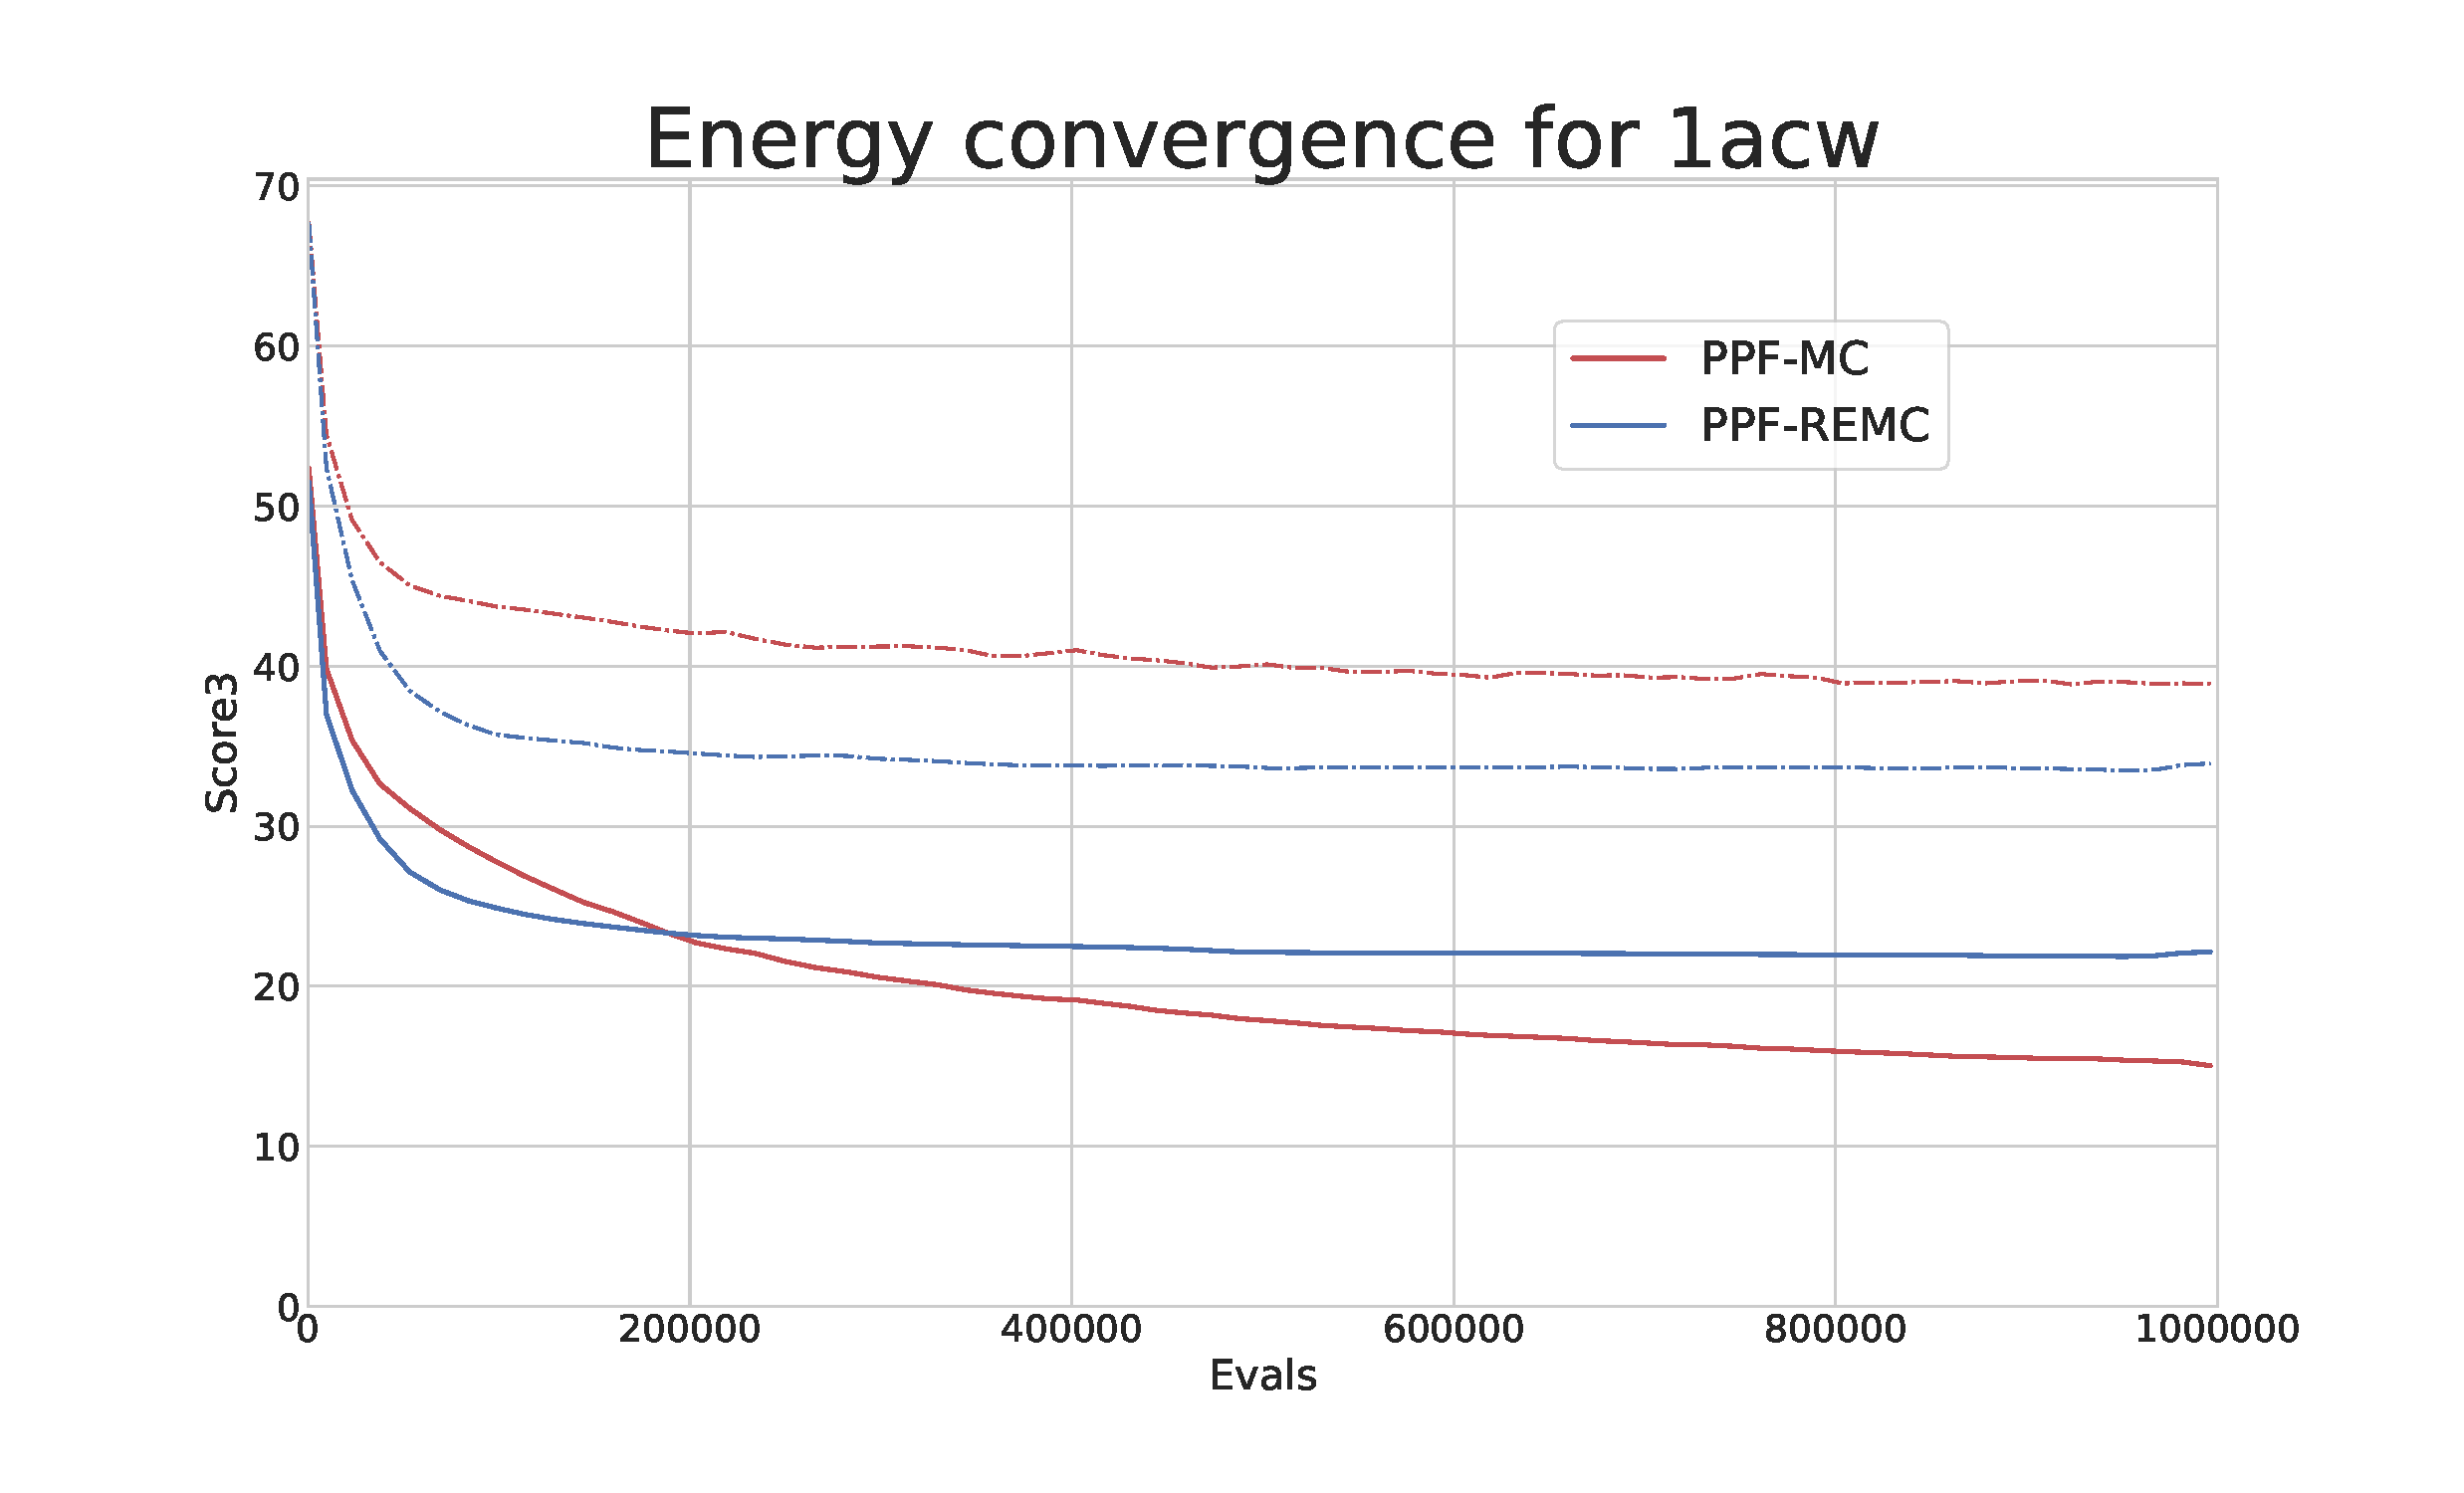
\includegraphics[width=1\linewidth]{Figuras/plots/energy_convergence/energy_convergence_1acw.pdf}
    \caption{1acw}
    %\label{fig:1acw-conformation}
  \end{subfigure}
%
  \begin{subfigure}{0.7\linewidth}
    \centering
    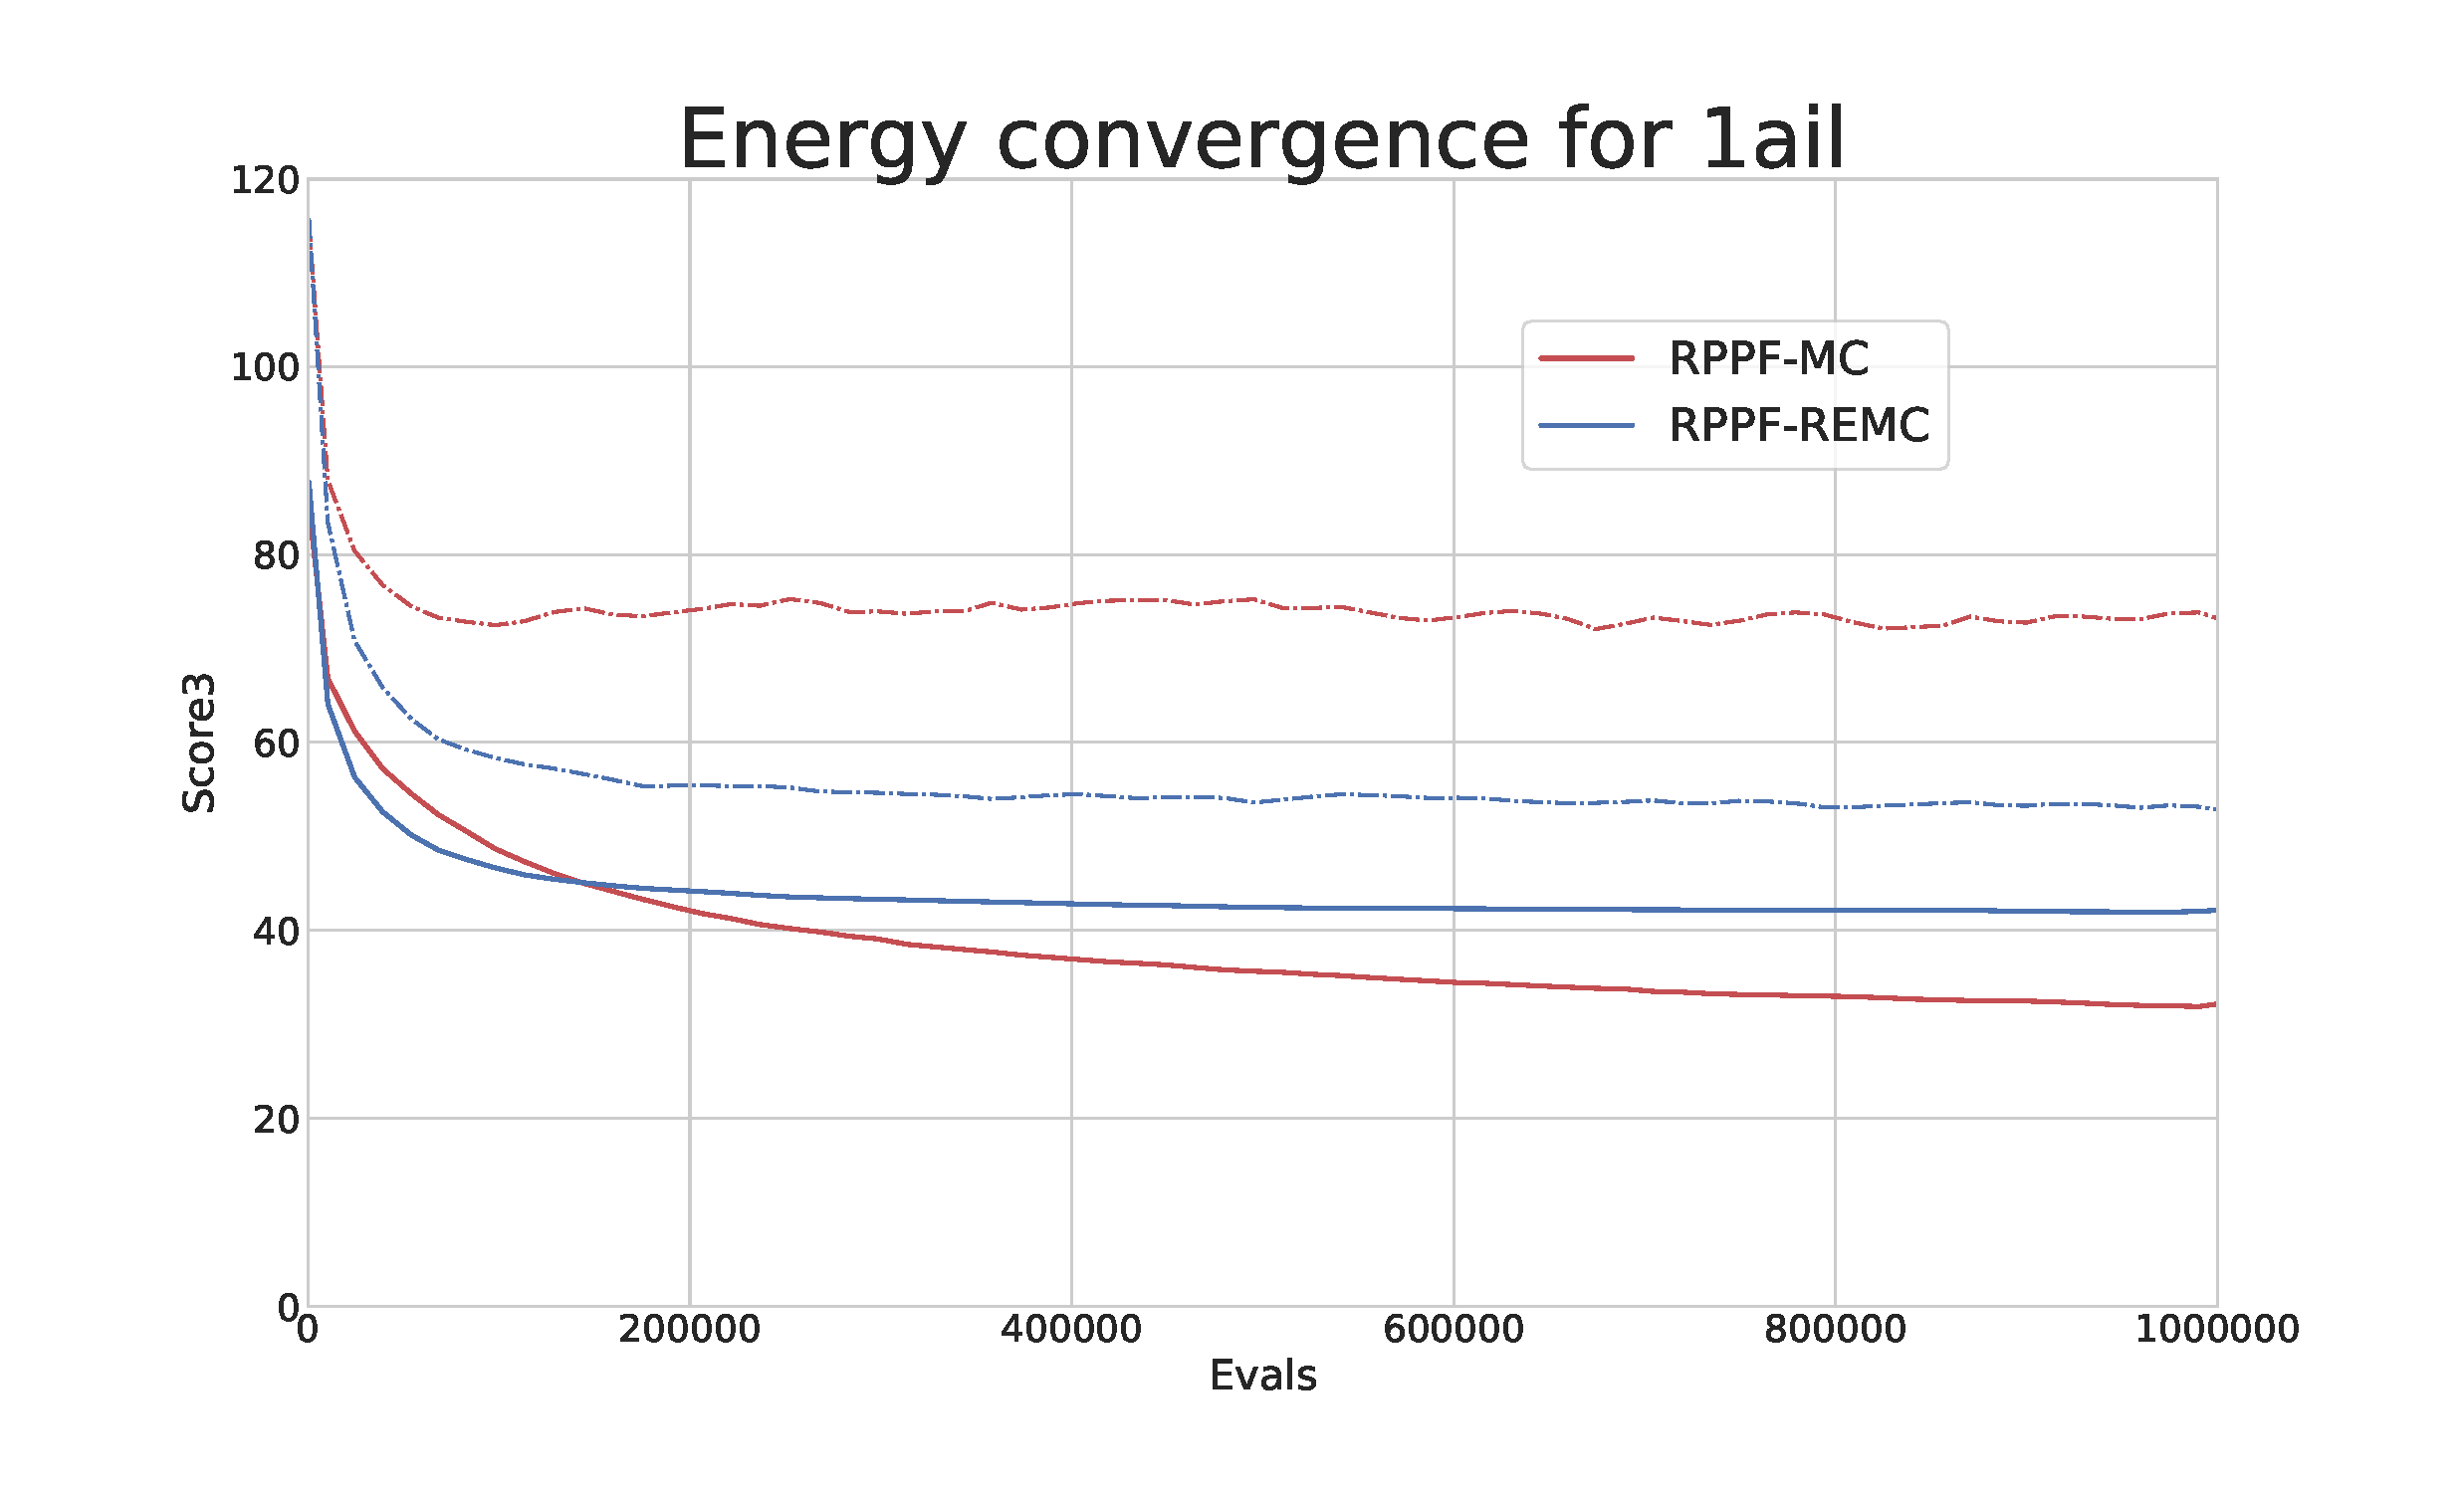
\includegraphics[width=1\linewidth]{Figuras/plots/energy_convergence/energy_convergence_1ail.pdf}
    \caption{1ail}
    %\label{fig:1acw-conformation}
  \end{subfigure}
%
  \begin{subfigure}{0.7\linewidth}
    \centering
    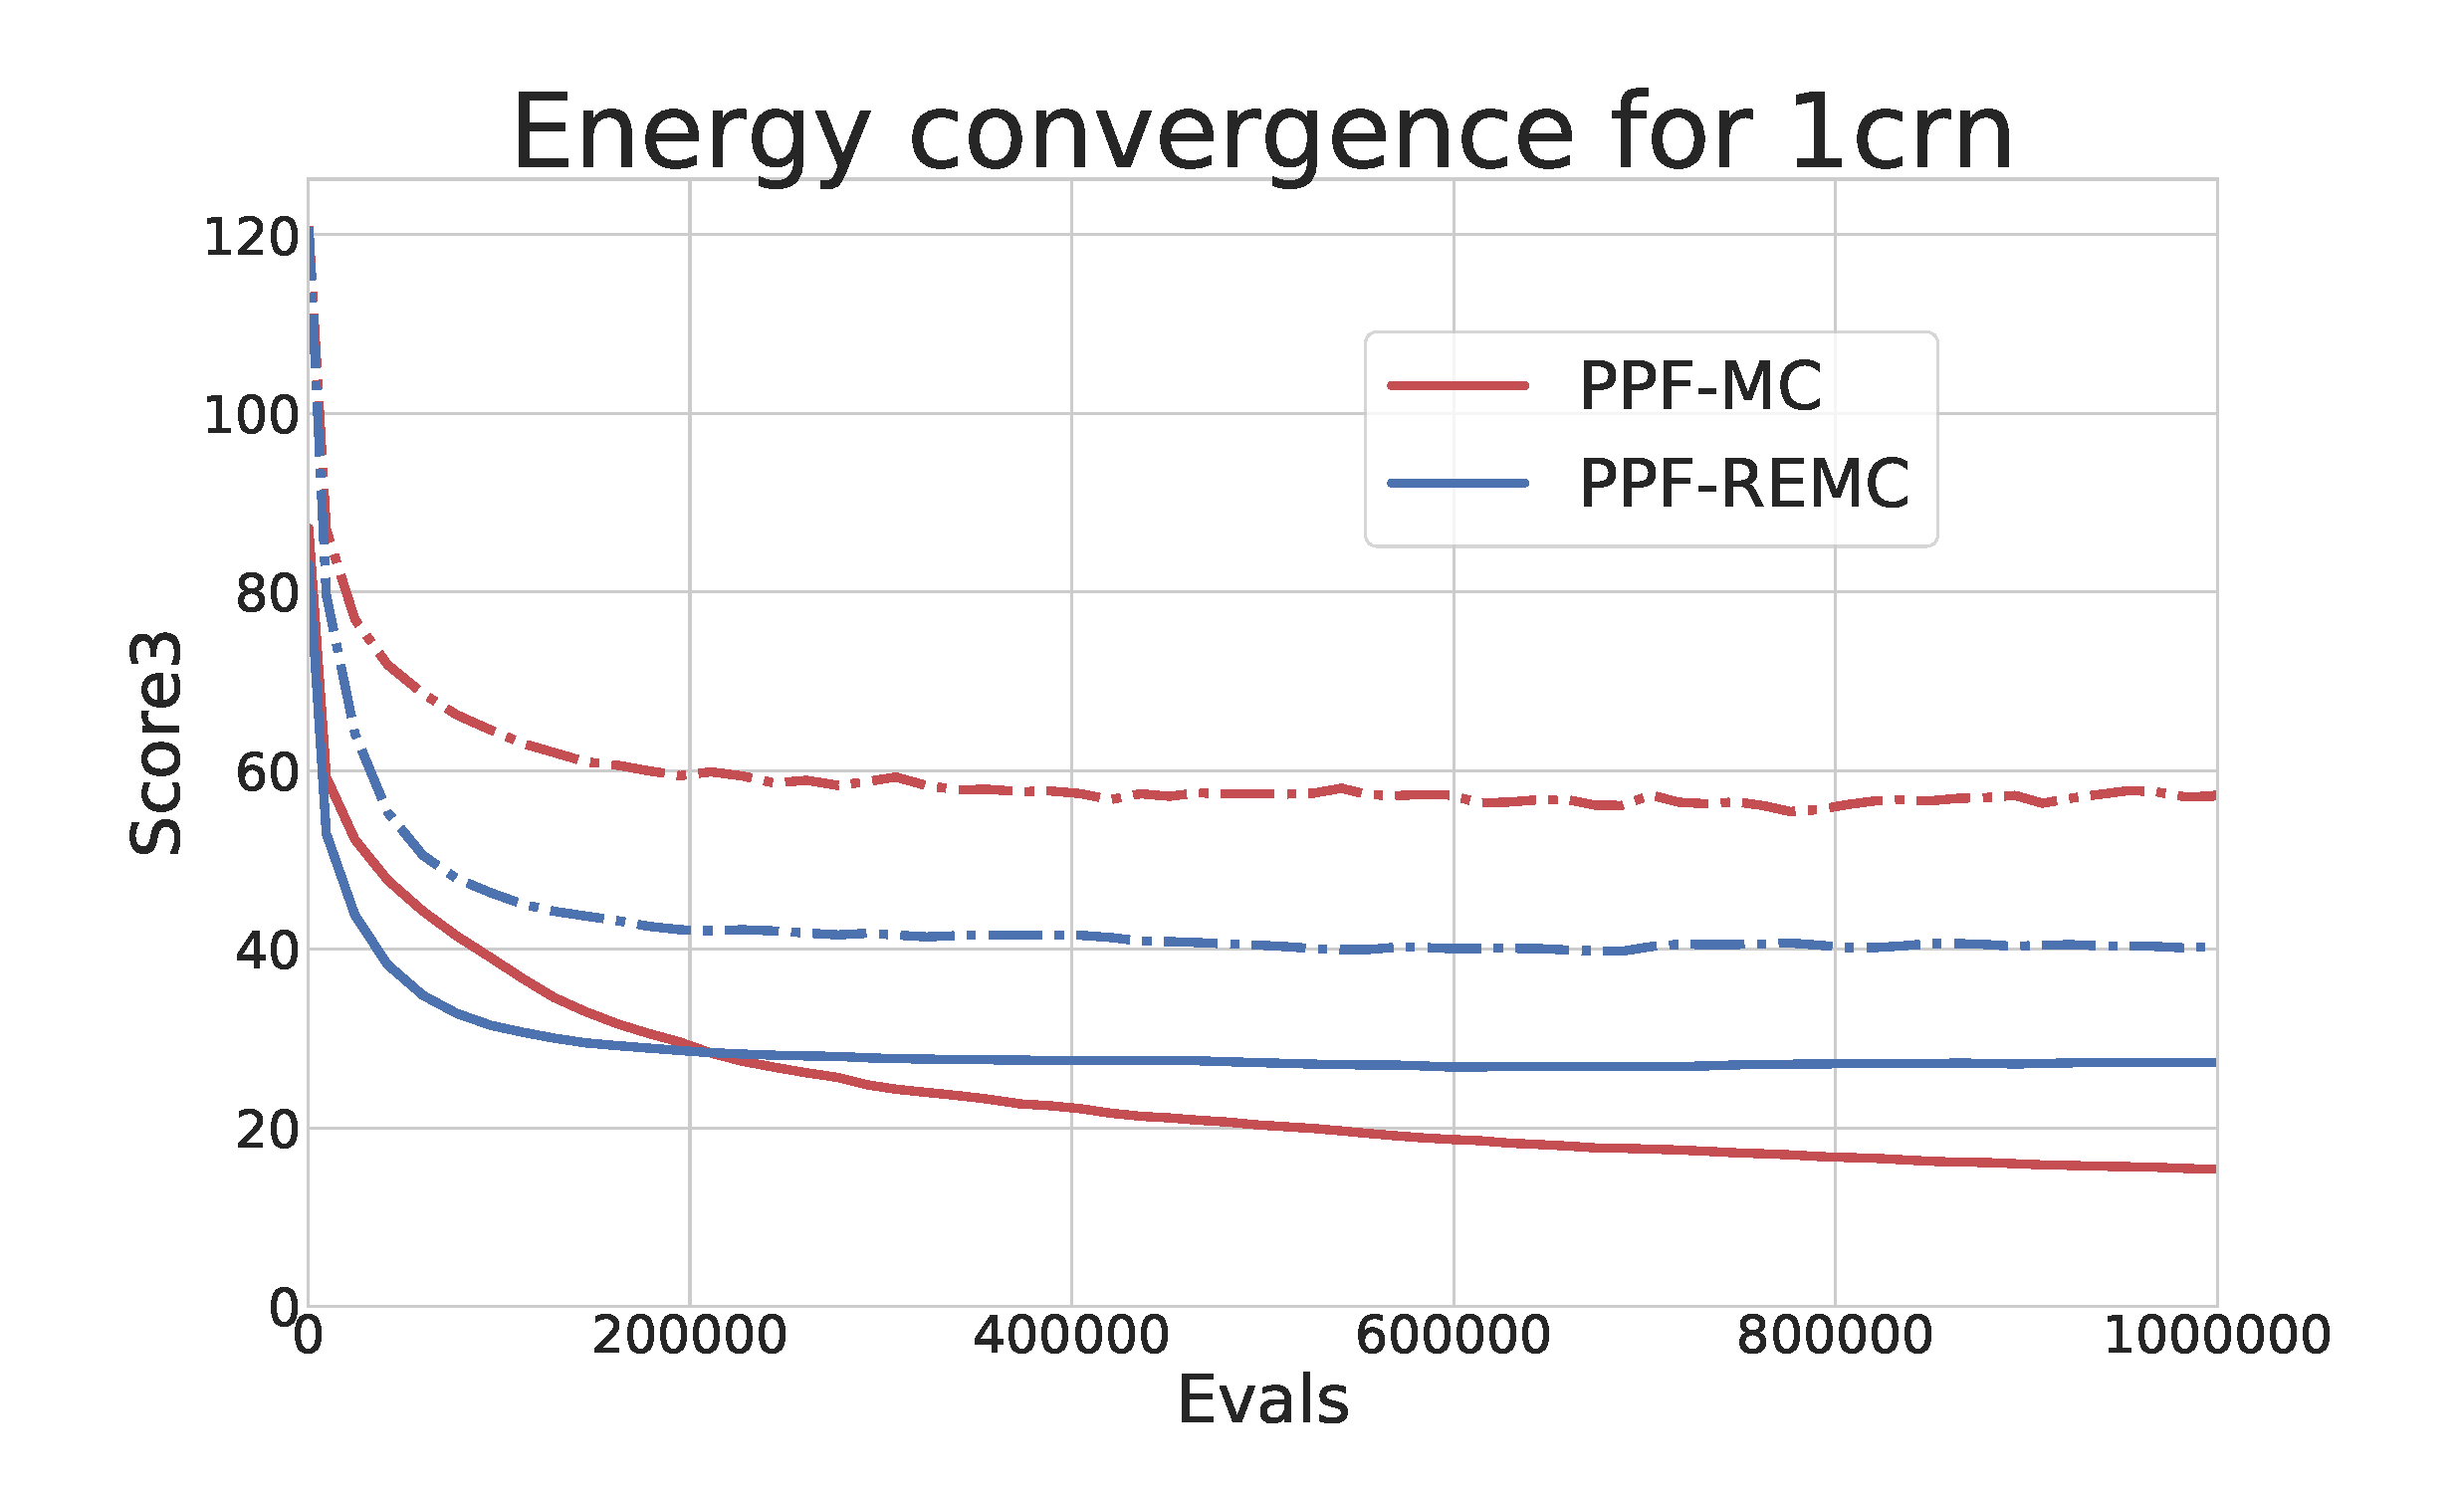
\includegraphics[width=1\linewidth]{Figuras/plots/energy_convergence/energy_convergence_1crn.pdf}
    \caption{1crn}
    %\label{fig:1acw-conformation}
  \end{subfigure}
\end{figure}

\begin{figure}[ht]\ContinuedFloat
  \begin{subfigure}{0.7\linewidth}
    \centering
    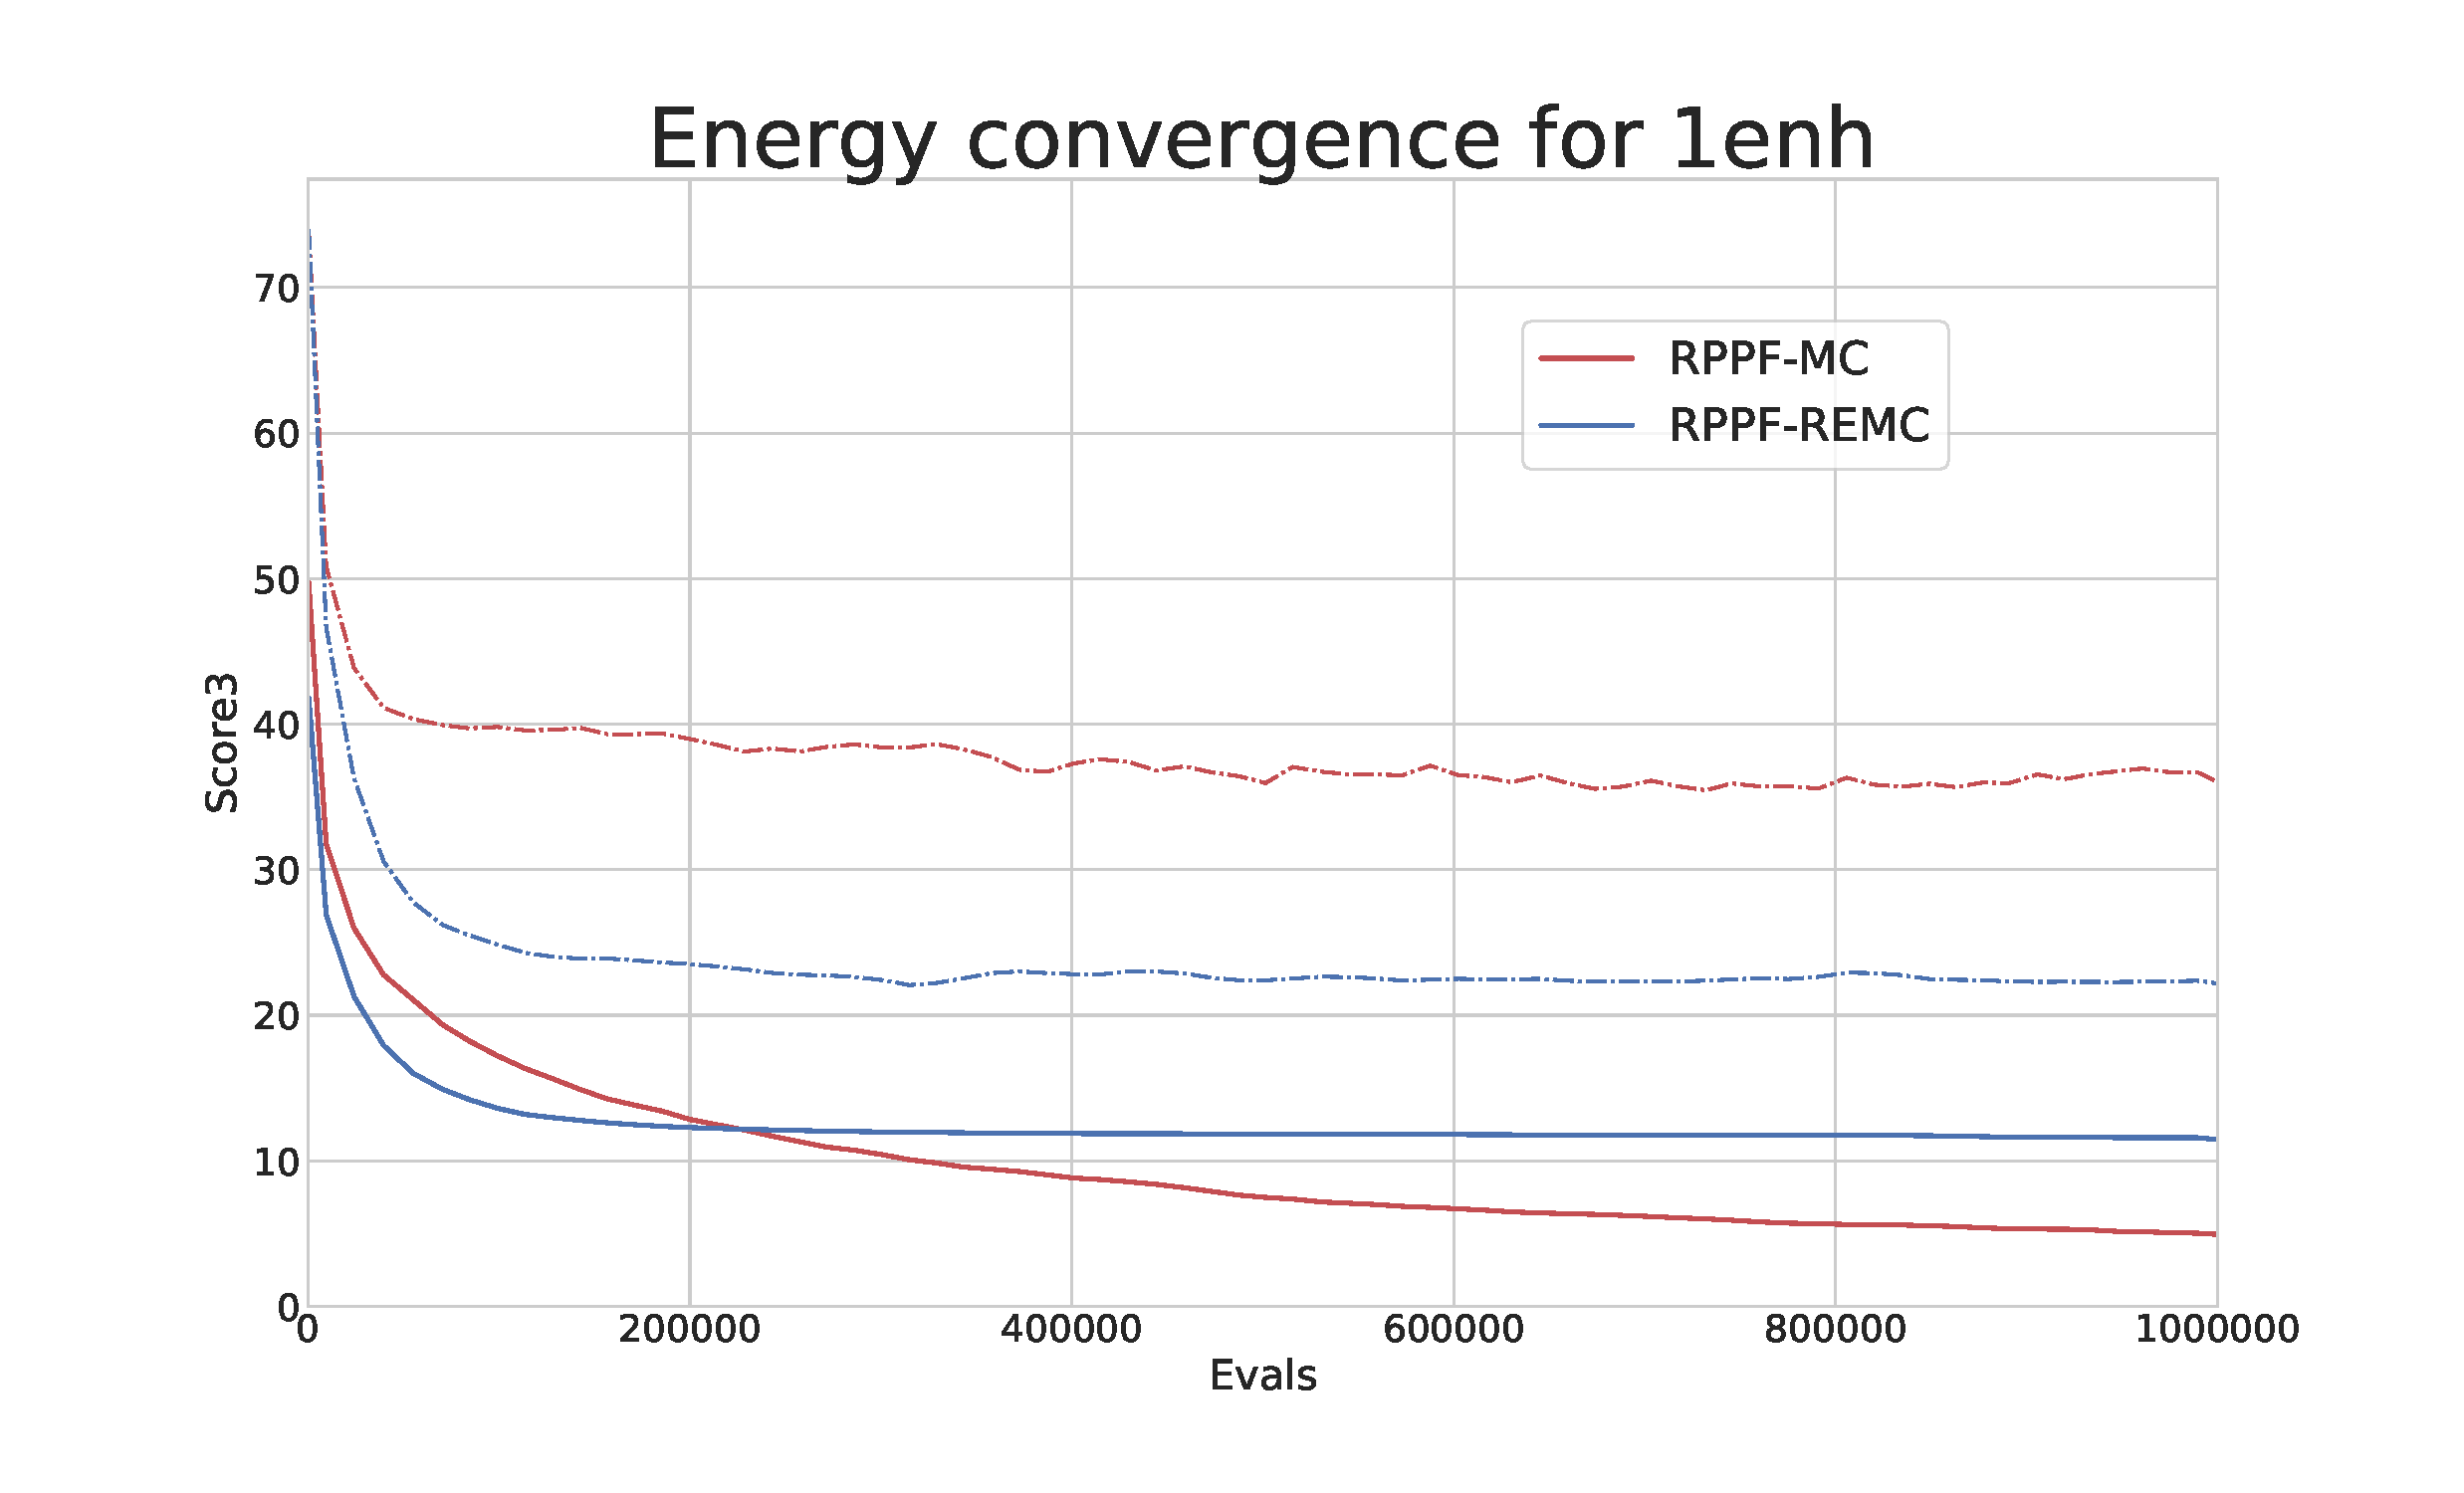
\includegraphics[width=1\linewidth]{Figuras/plots/energy_convergence/energy_convergence_1enh.pdf}
    \caption{1enh}
    %\label{fig:1acw-conformation}
  \end{subfigure}
%
  \begin{subfigure}{0.7\linewidth}
    \centering
    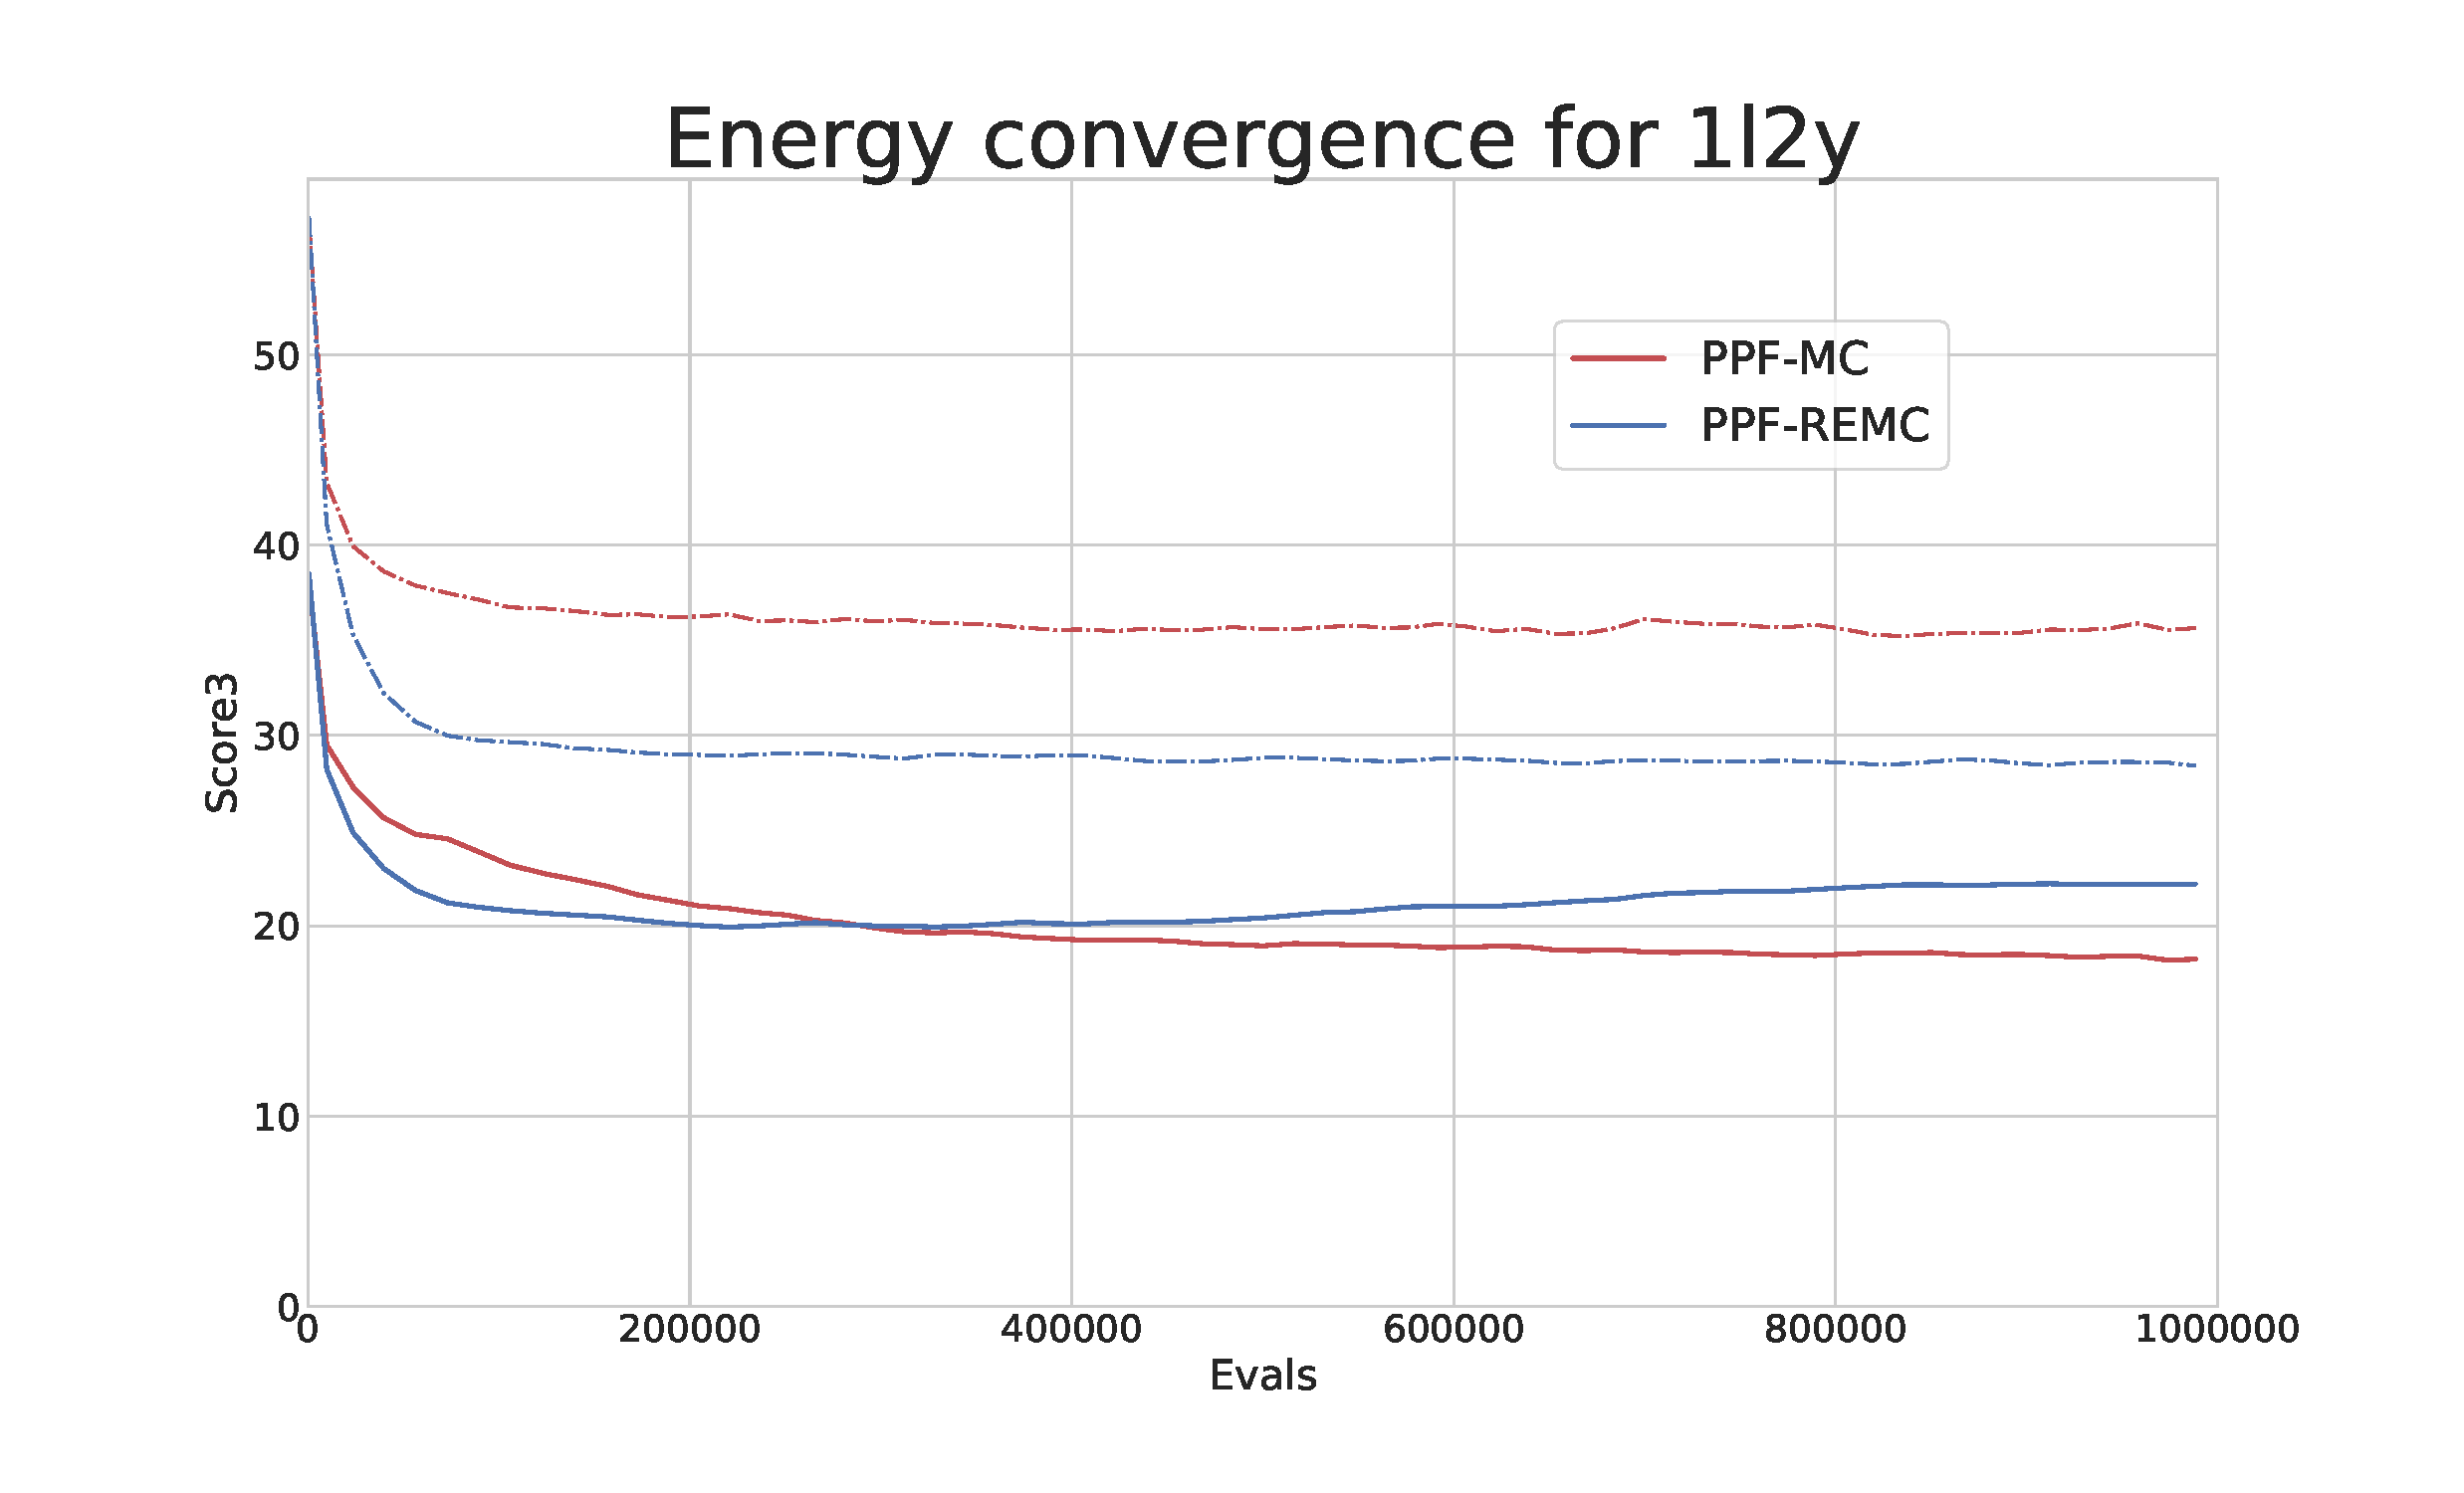
\includegraphics[width=1\linewidth]{Figuras/plots/energy_convergence/energy_convergence_1l2y.pdf}
    \caption{1utg}
    %\label{fig:1acw-conformation}
  \end{subfigure}
%
  \begin{subfigure}{0.7\linewidth}
    \centering
    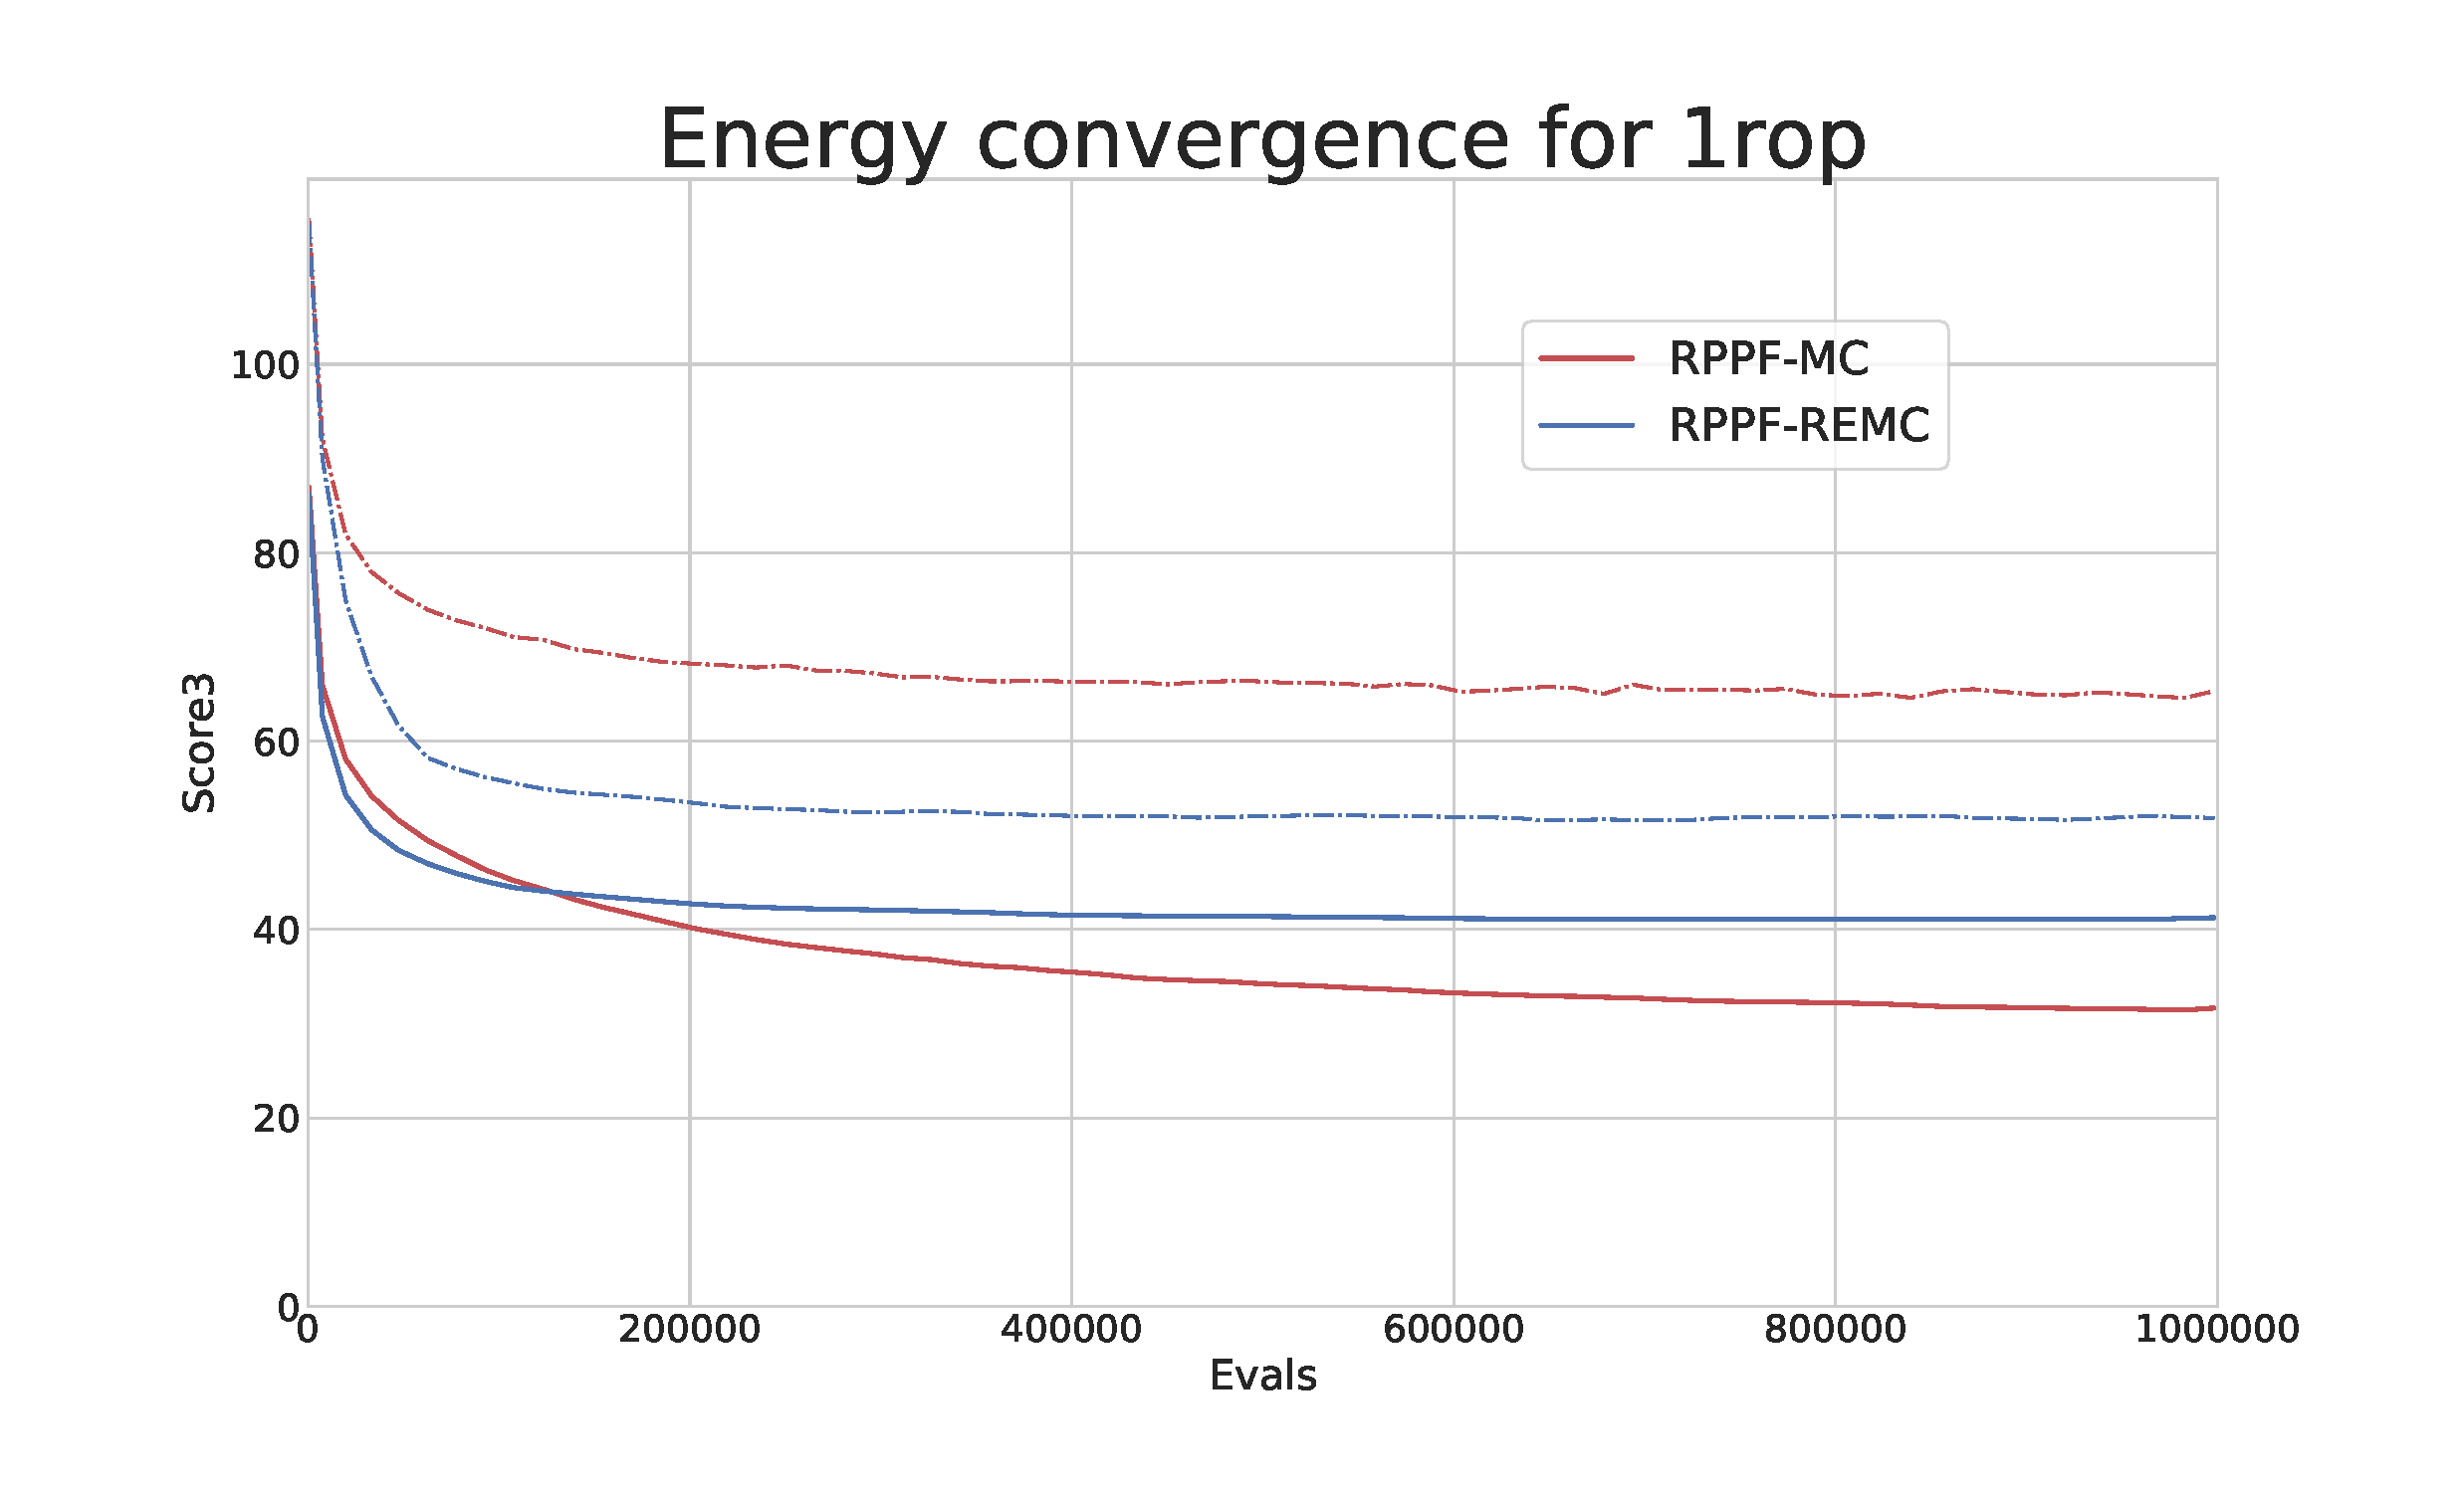
\includegraphics[width=1\linewidth]{Figuras/plots/energy_convergence/energy_convergence_1rop.pdf}
    \caption{1rop}
    %\label{fig:1acw-conformation}
  \end{subfigure}
\end{figure}

\begin{figure}[ht]\ContinuedFloat
  \begin{subfigure}{0.7\linewidth}
    \centering
    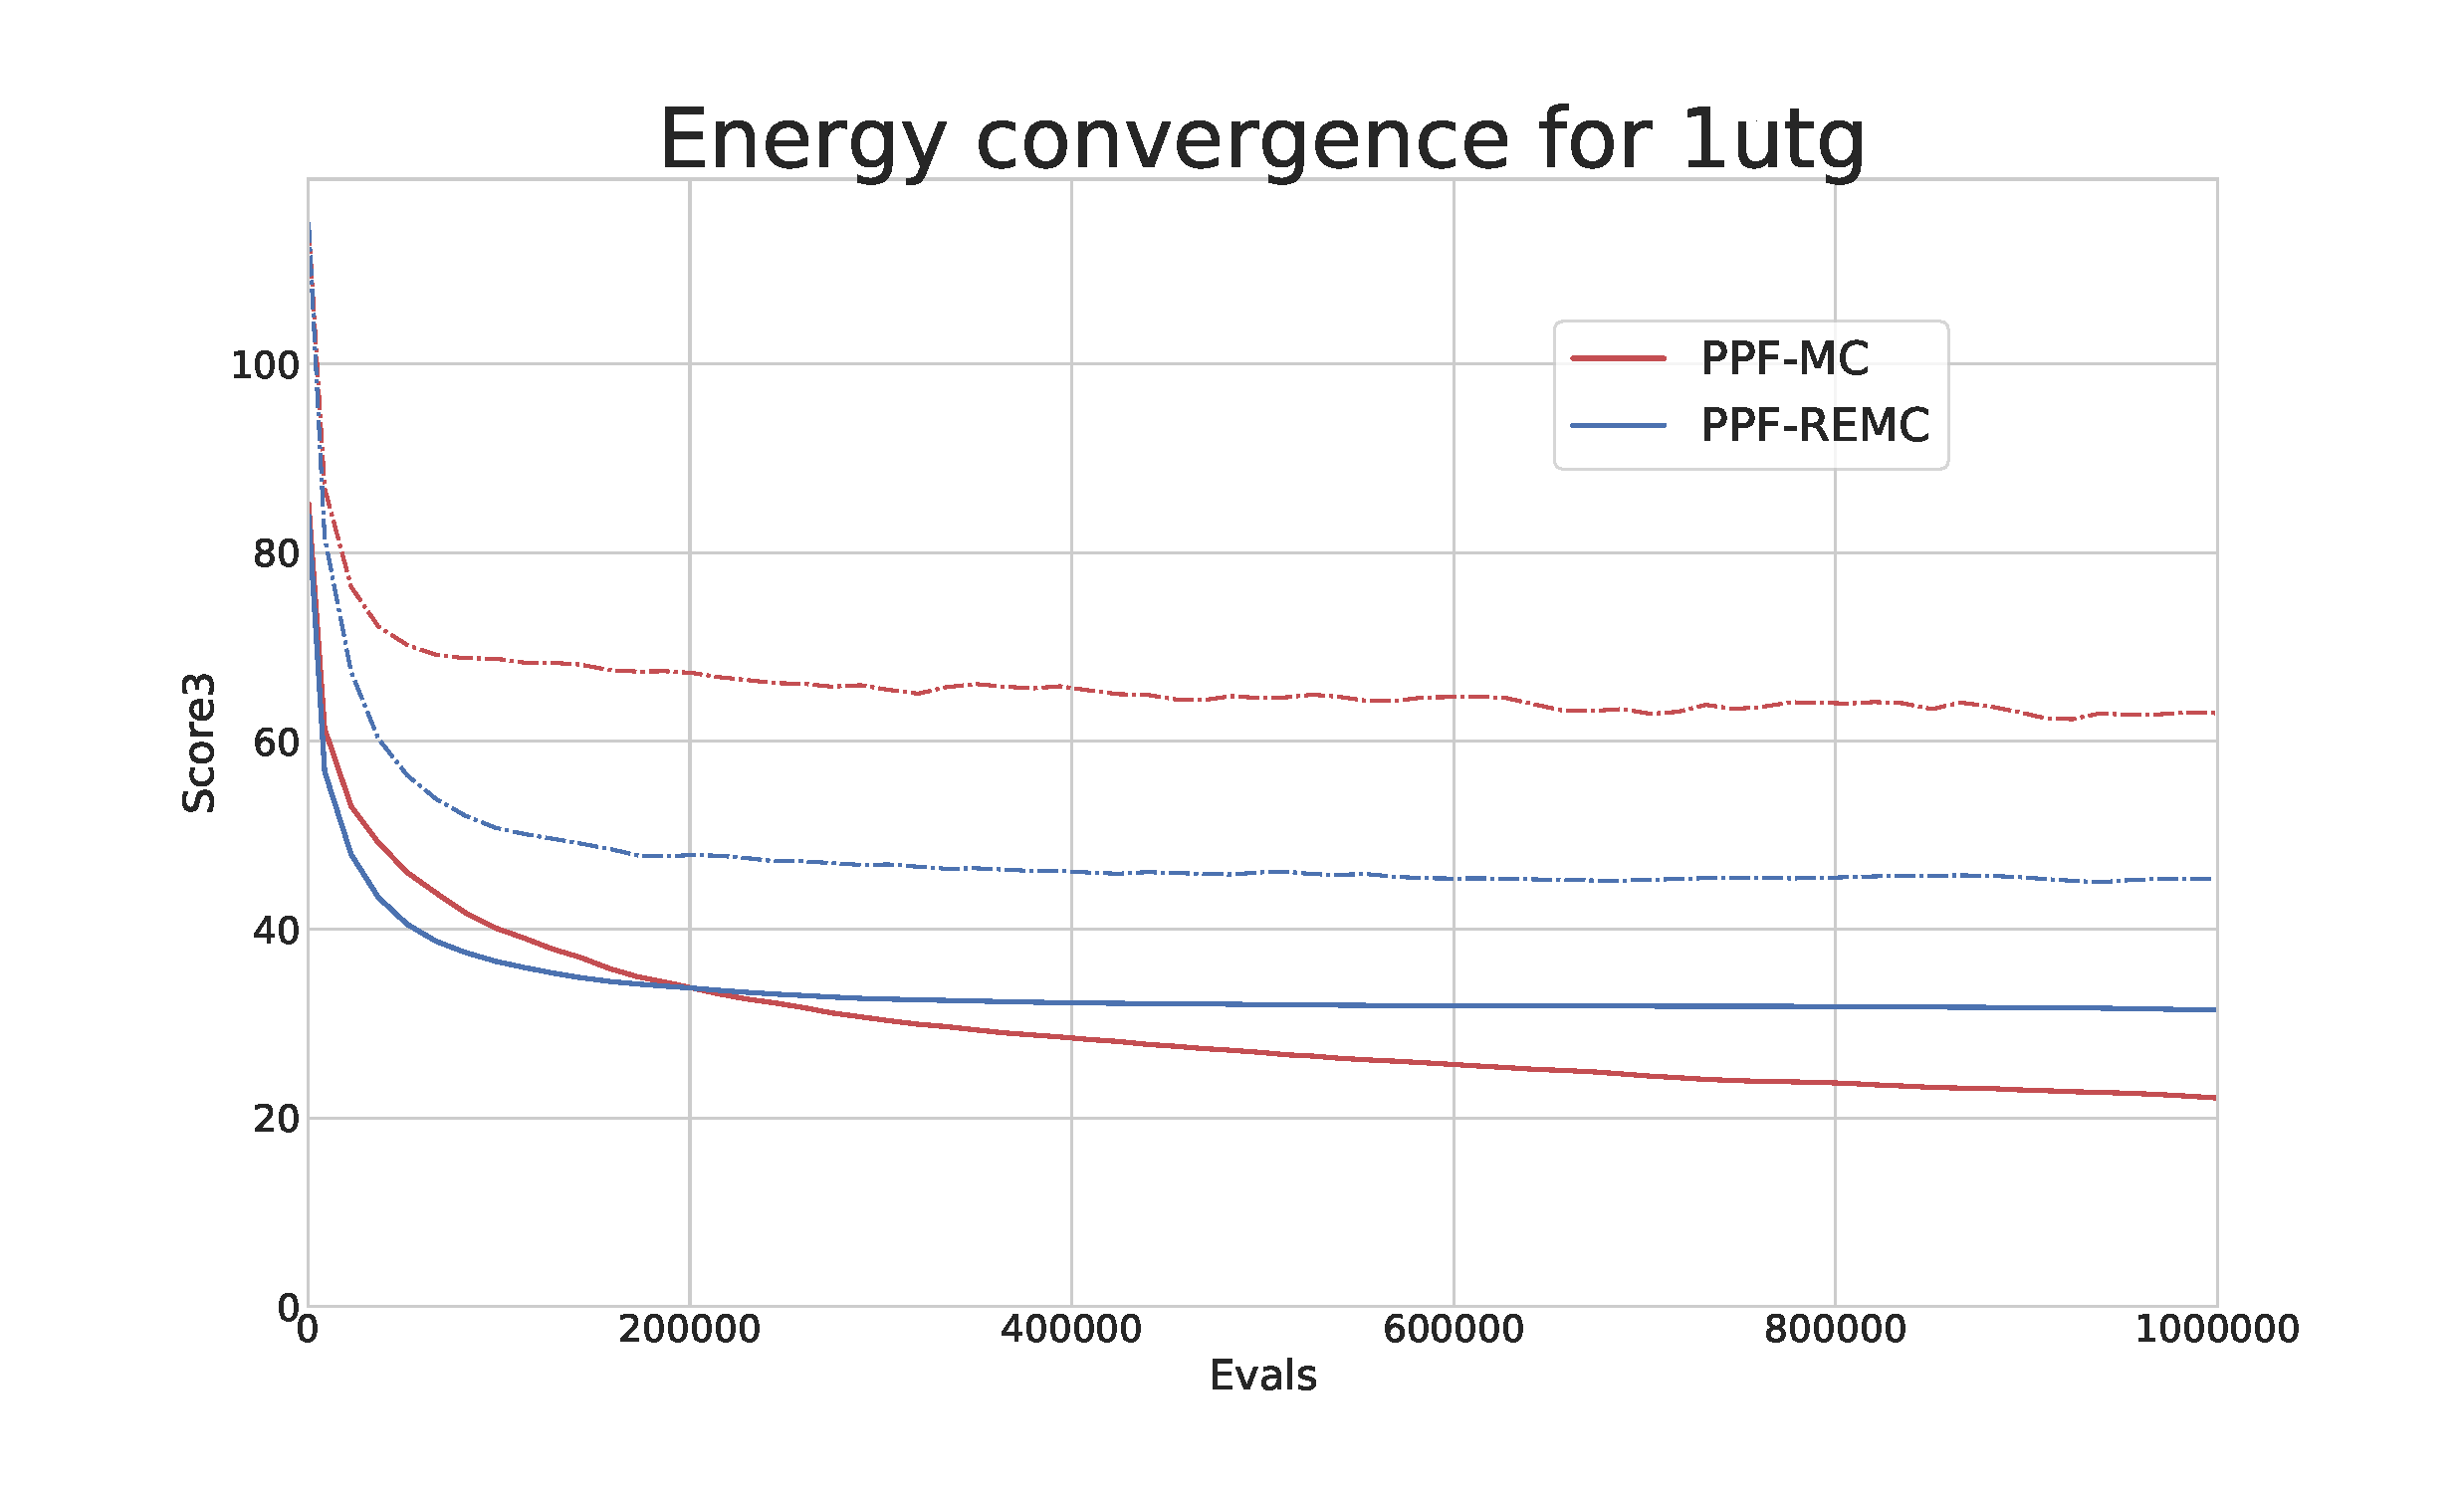
\includegraphics[width=1\linewidth]{Figuras/plots/energy_convergence/energy_convergence_1utg.pdf}
    \caption{1utg}
    %\label{fig:1utg-conformation}
  \end{subfigure}
%
  \begin{subfigure}{0.7\linewidth}
    \centering
    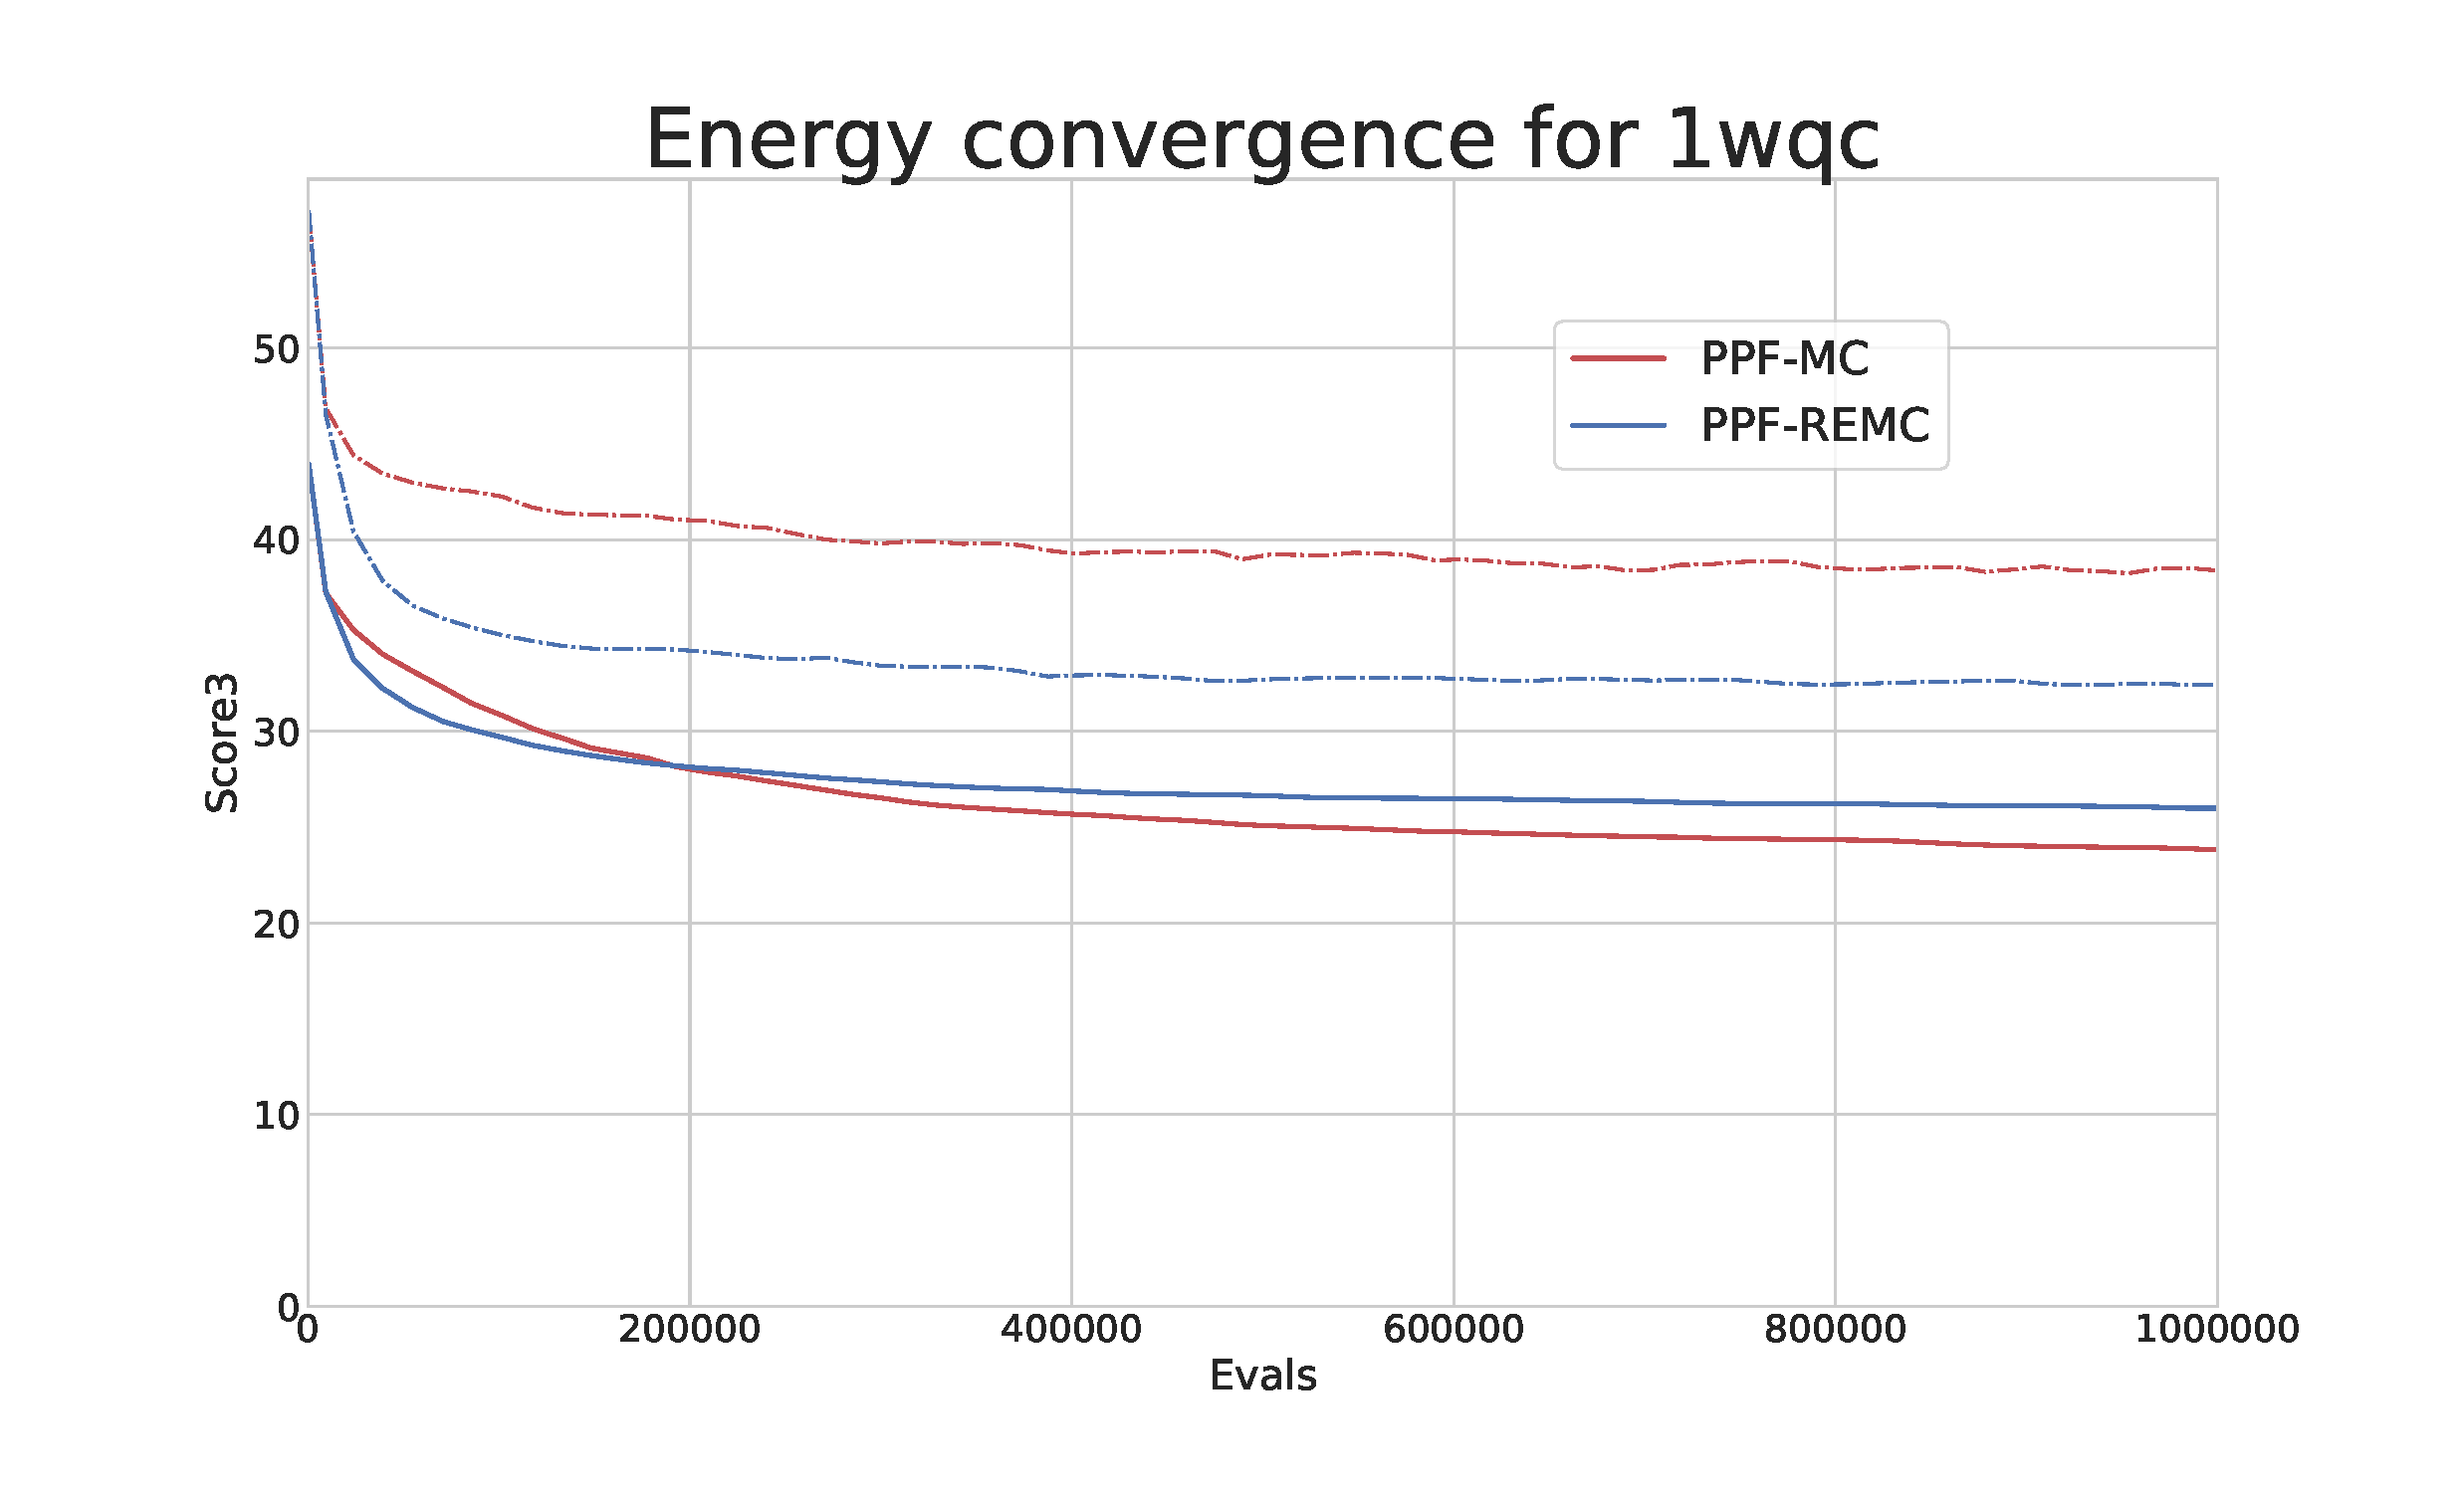
\includegraphics[width=1\linewidth]{Figuras/plots/energy_convergence/energy_convergence_1wqc.pdf}
    \caption{1wqc}
    %\label{fig:1wqc-conformation}
  \end{subfigure}
%
  \begin{subfigure}{0.7\linewidth}
    \centering
    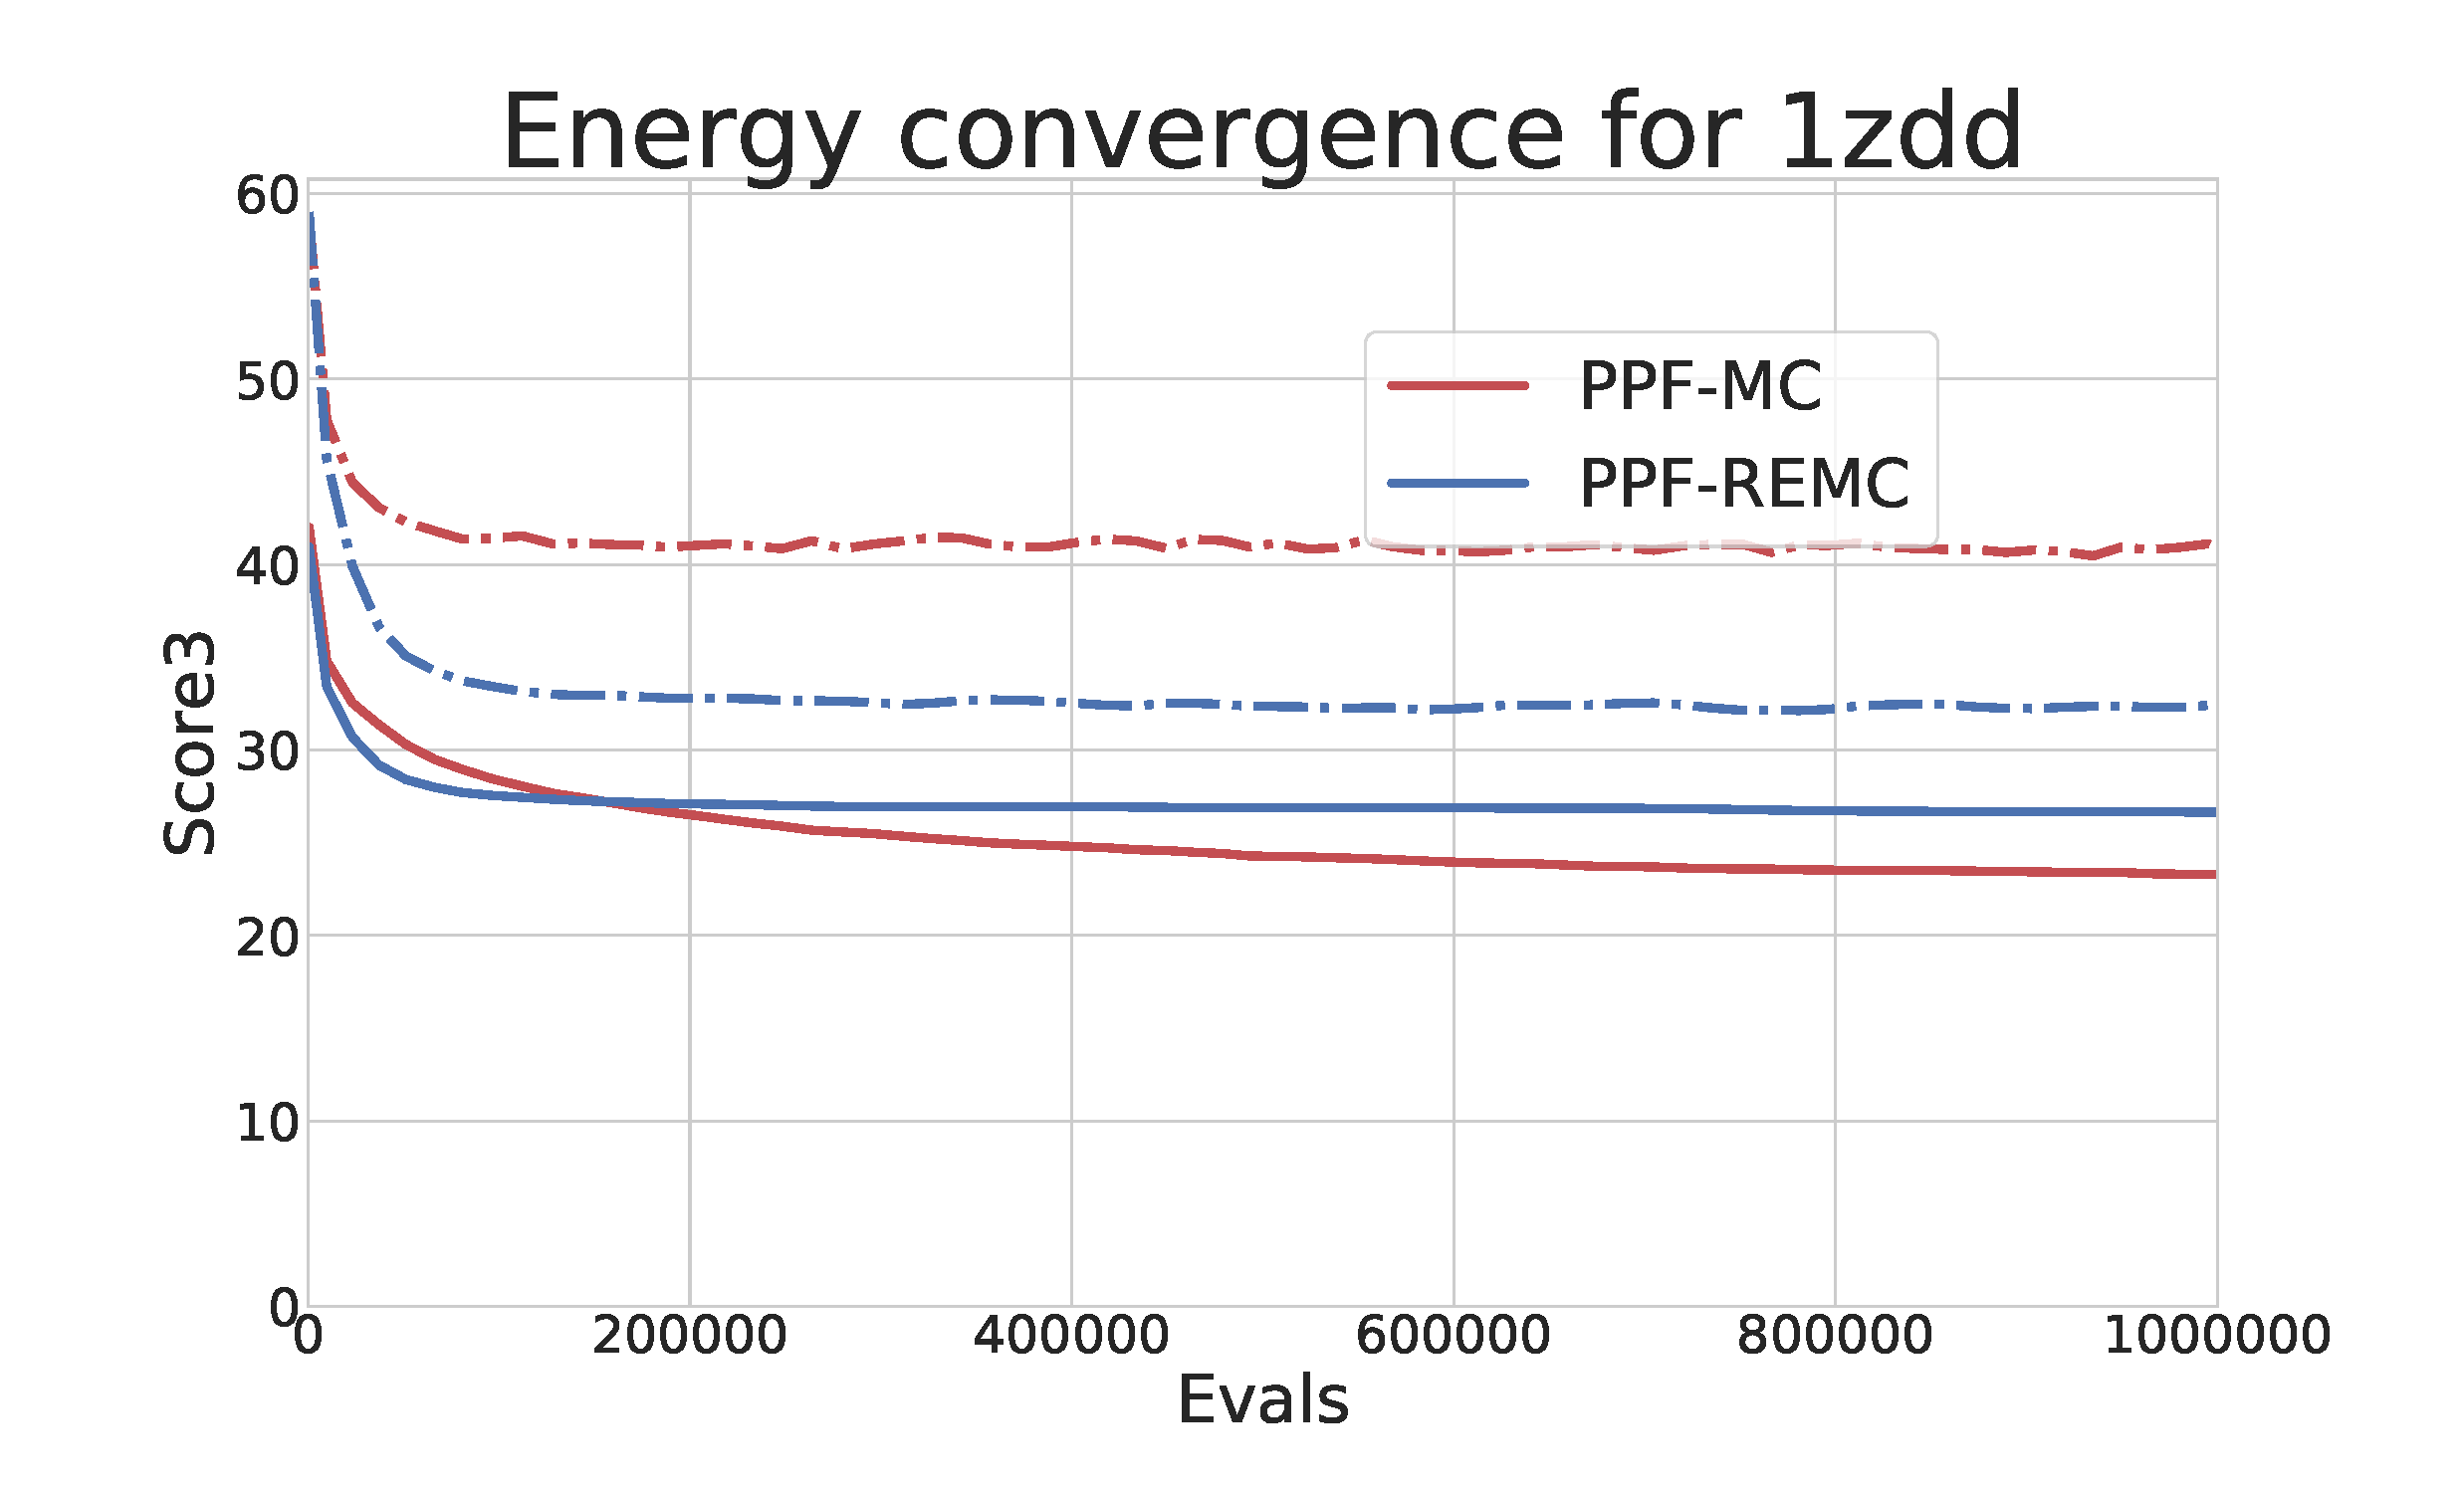
\includegraphics[width=1\linewidth]{Figuras/plots/energy_convergence/energy_convergence_1zdd.pdf}
    \caption{1zdd}
    %\label{fig:1zdd-conformation}
  \end{subfigure}
\end{figure}

\begin{figure}[ht]\ContinuedFloat
  \begin{subfigure}{0.7\linewidth}
    \centering
    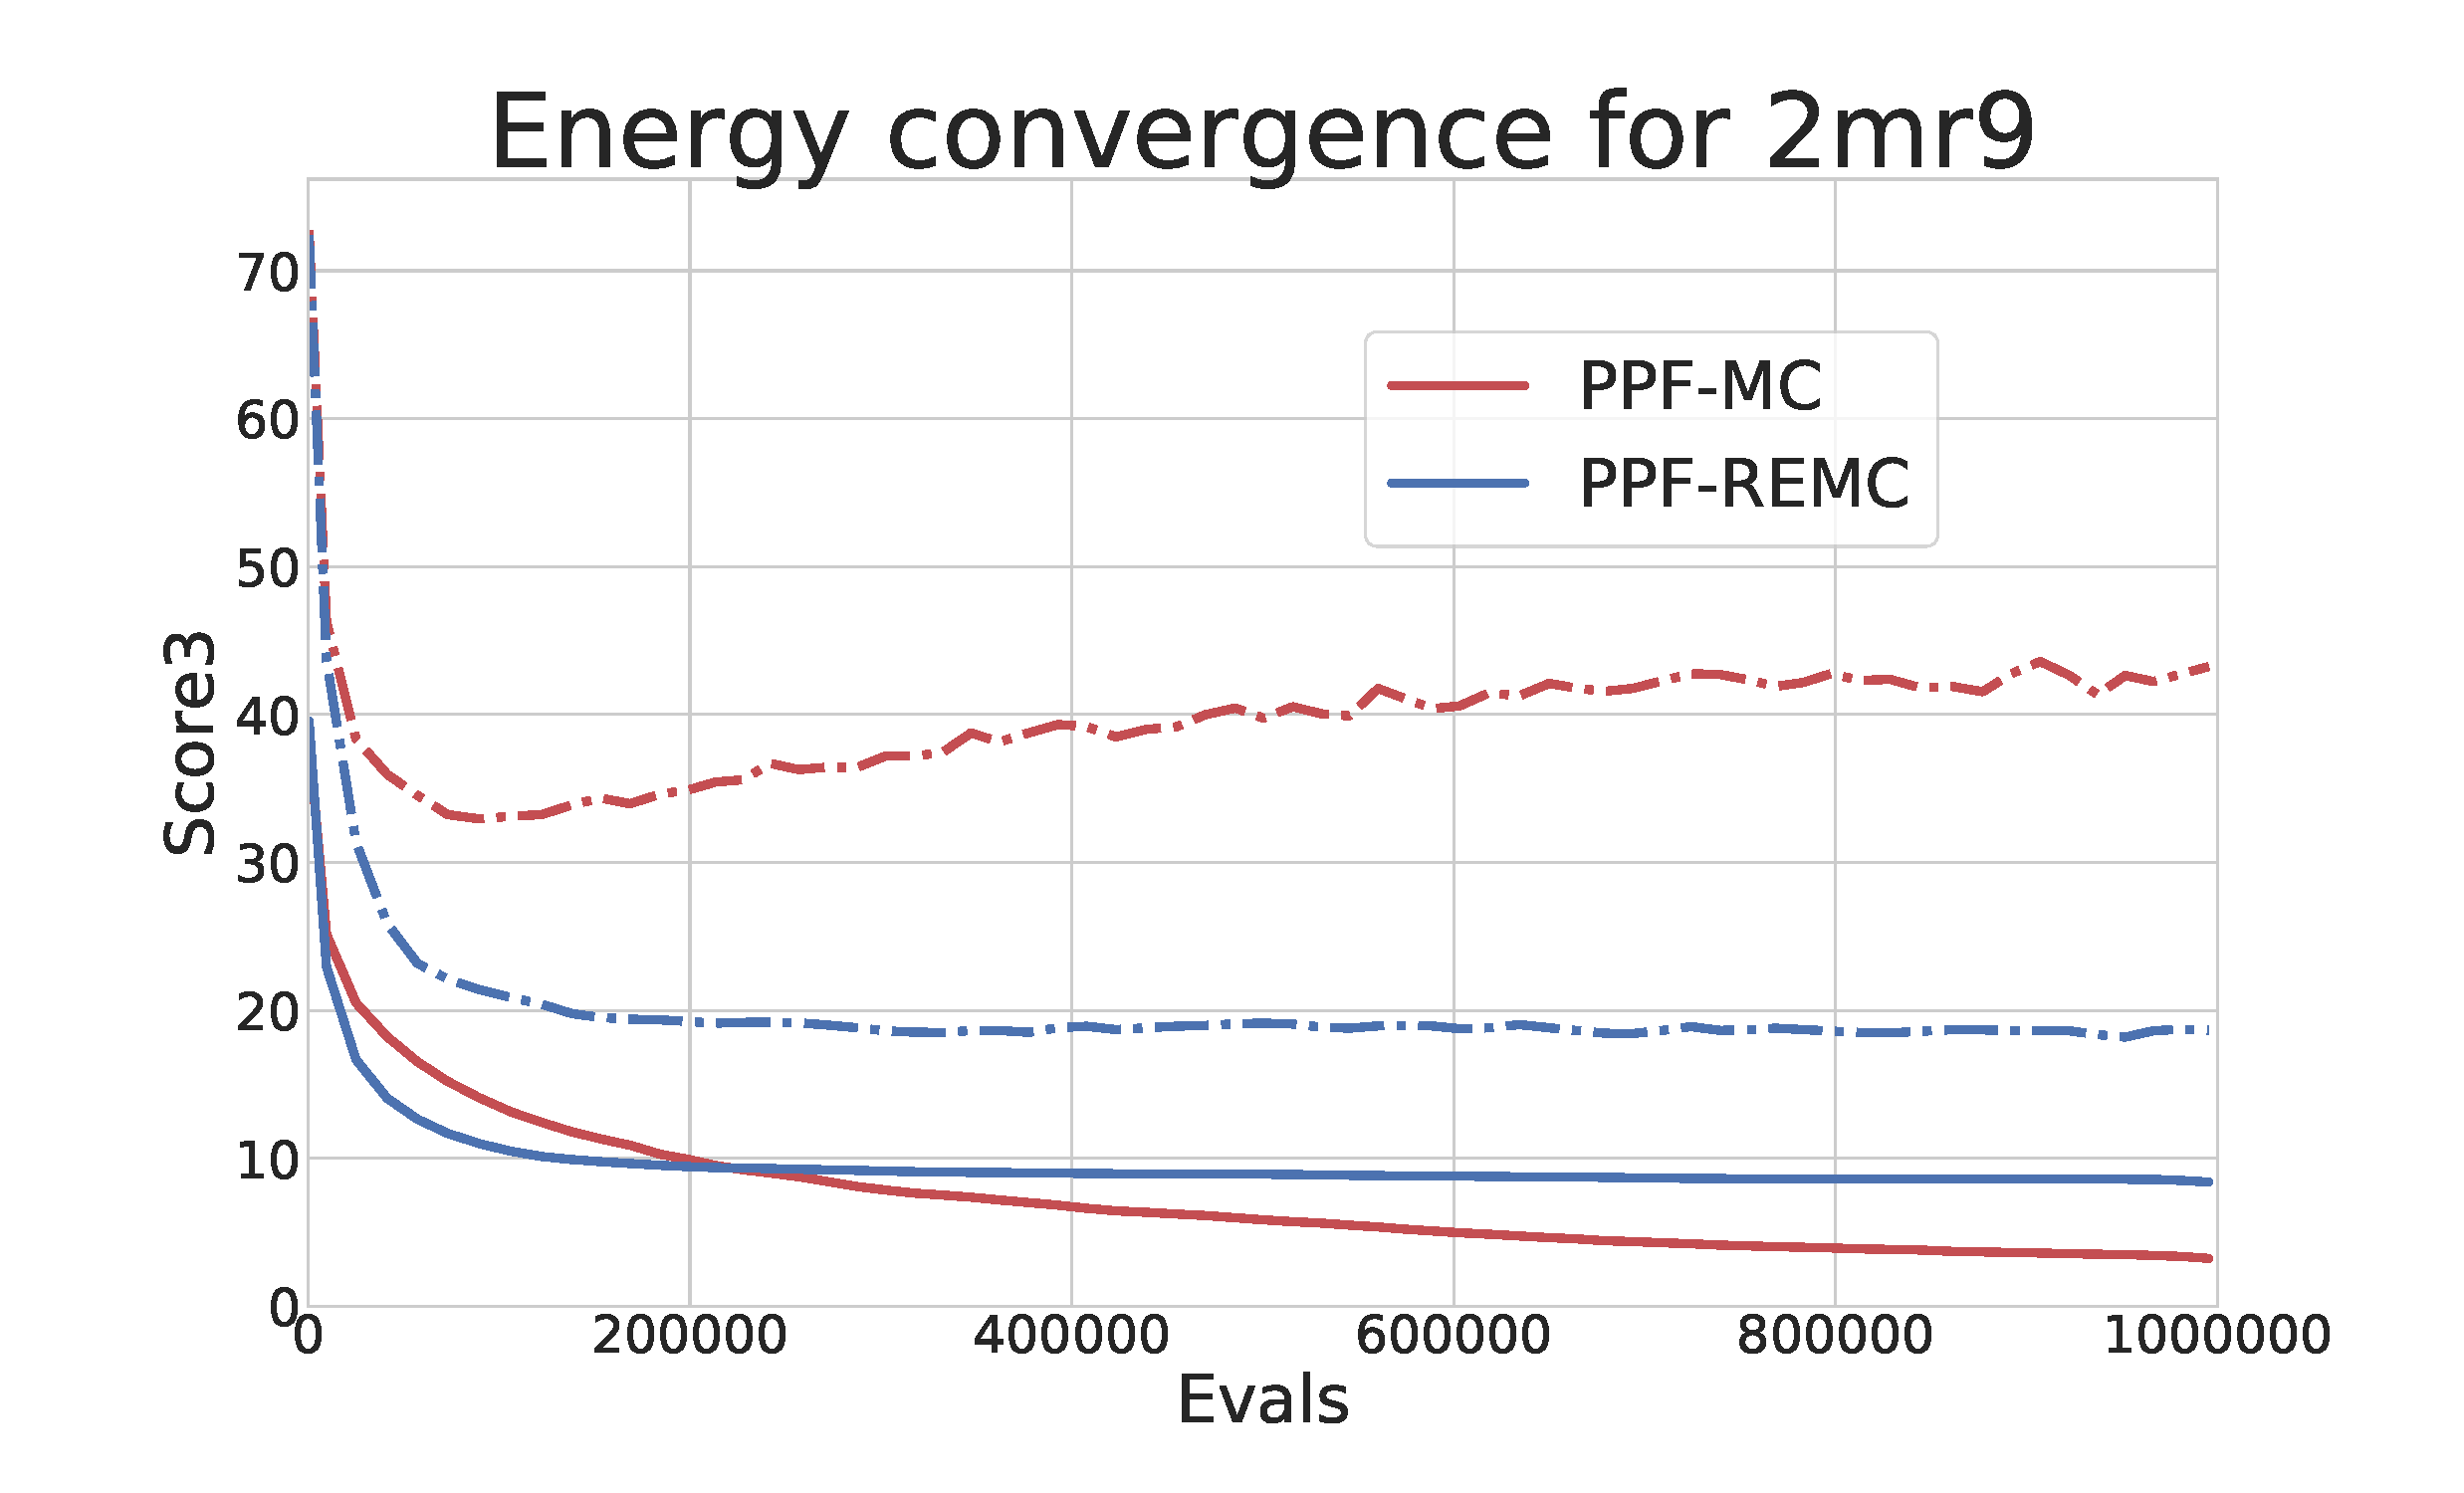
\includegraphics[width=1\linewidth]{Figuras/plots/energy_convergence/energy_convergence_2mr9.pdf}
    \caption{2mr9}
    %\label{fig:2mr9-conformation}
  \end{subfigure}
\end{figure}

\section{Average RMSD graphs}

\begin{figure}[ht]
  \begin{subfigure}{0.7\linewidth}
    \centering
    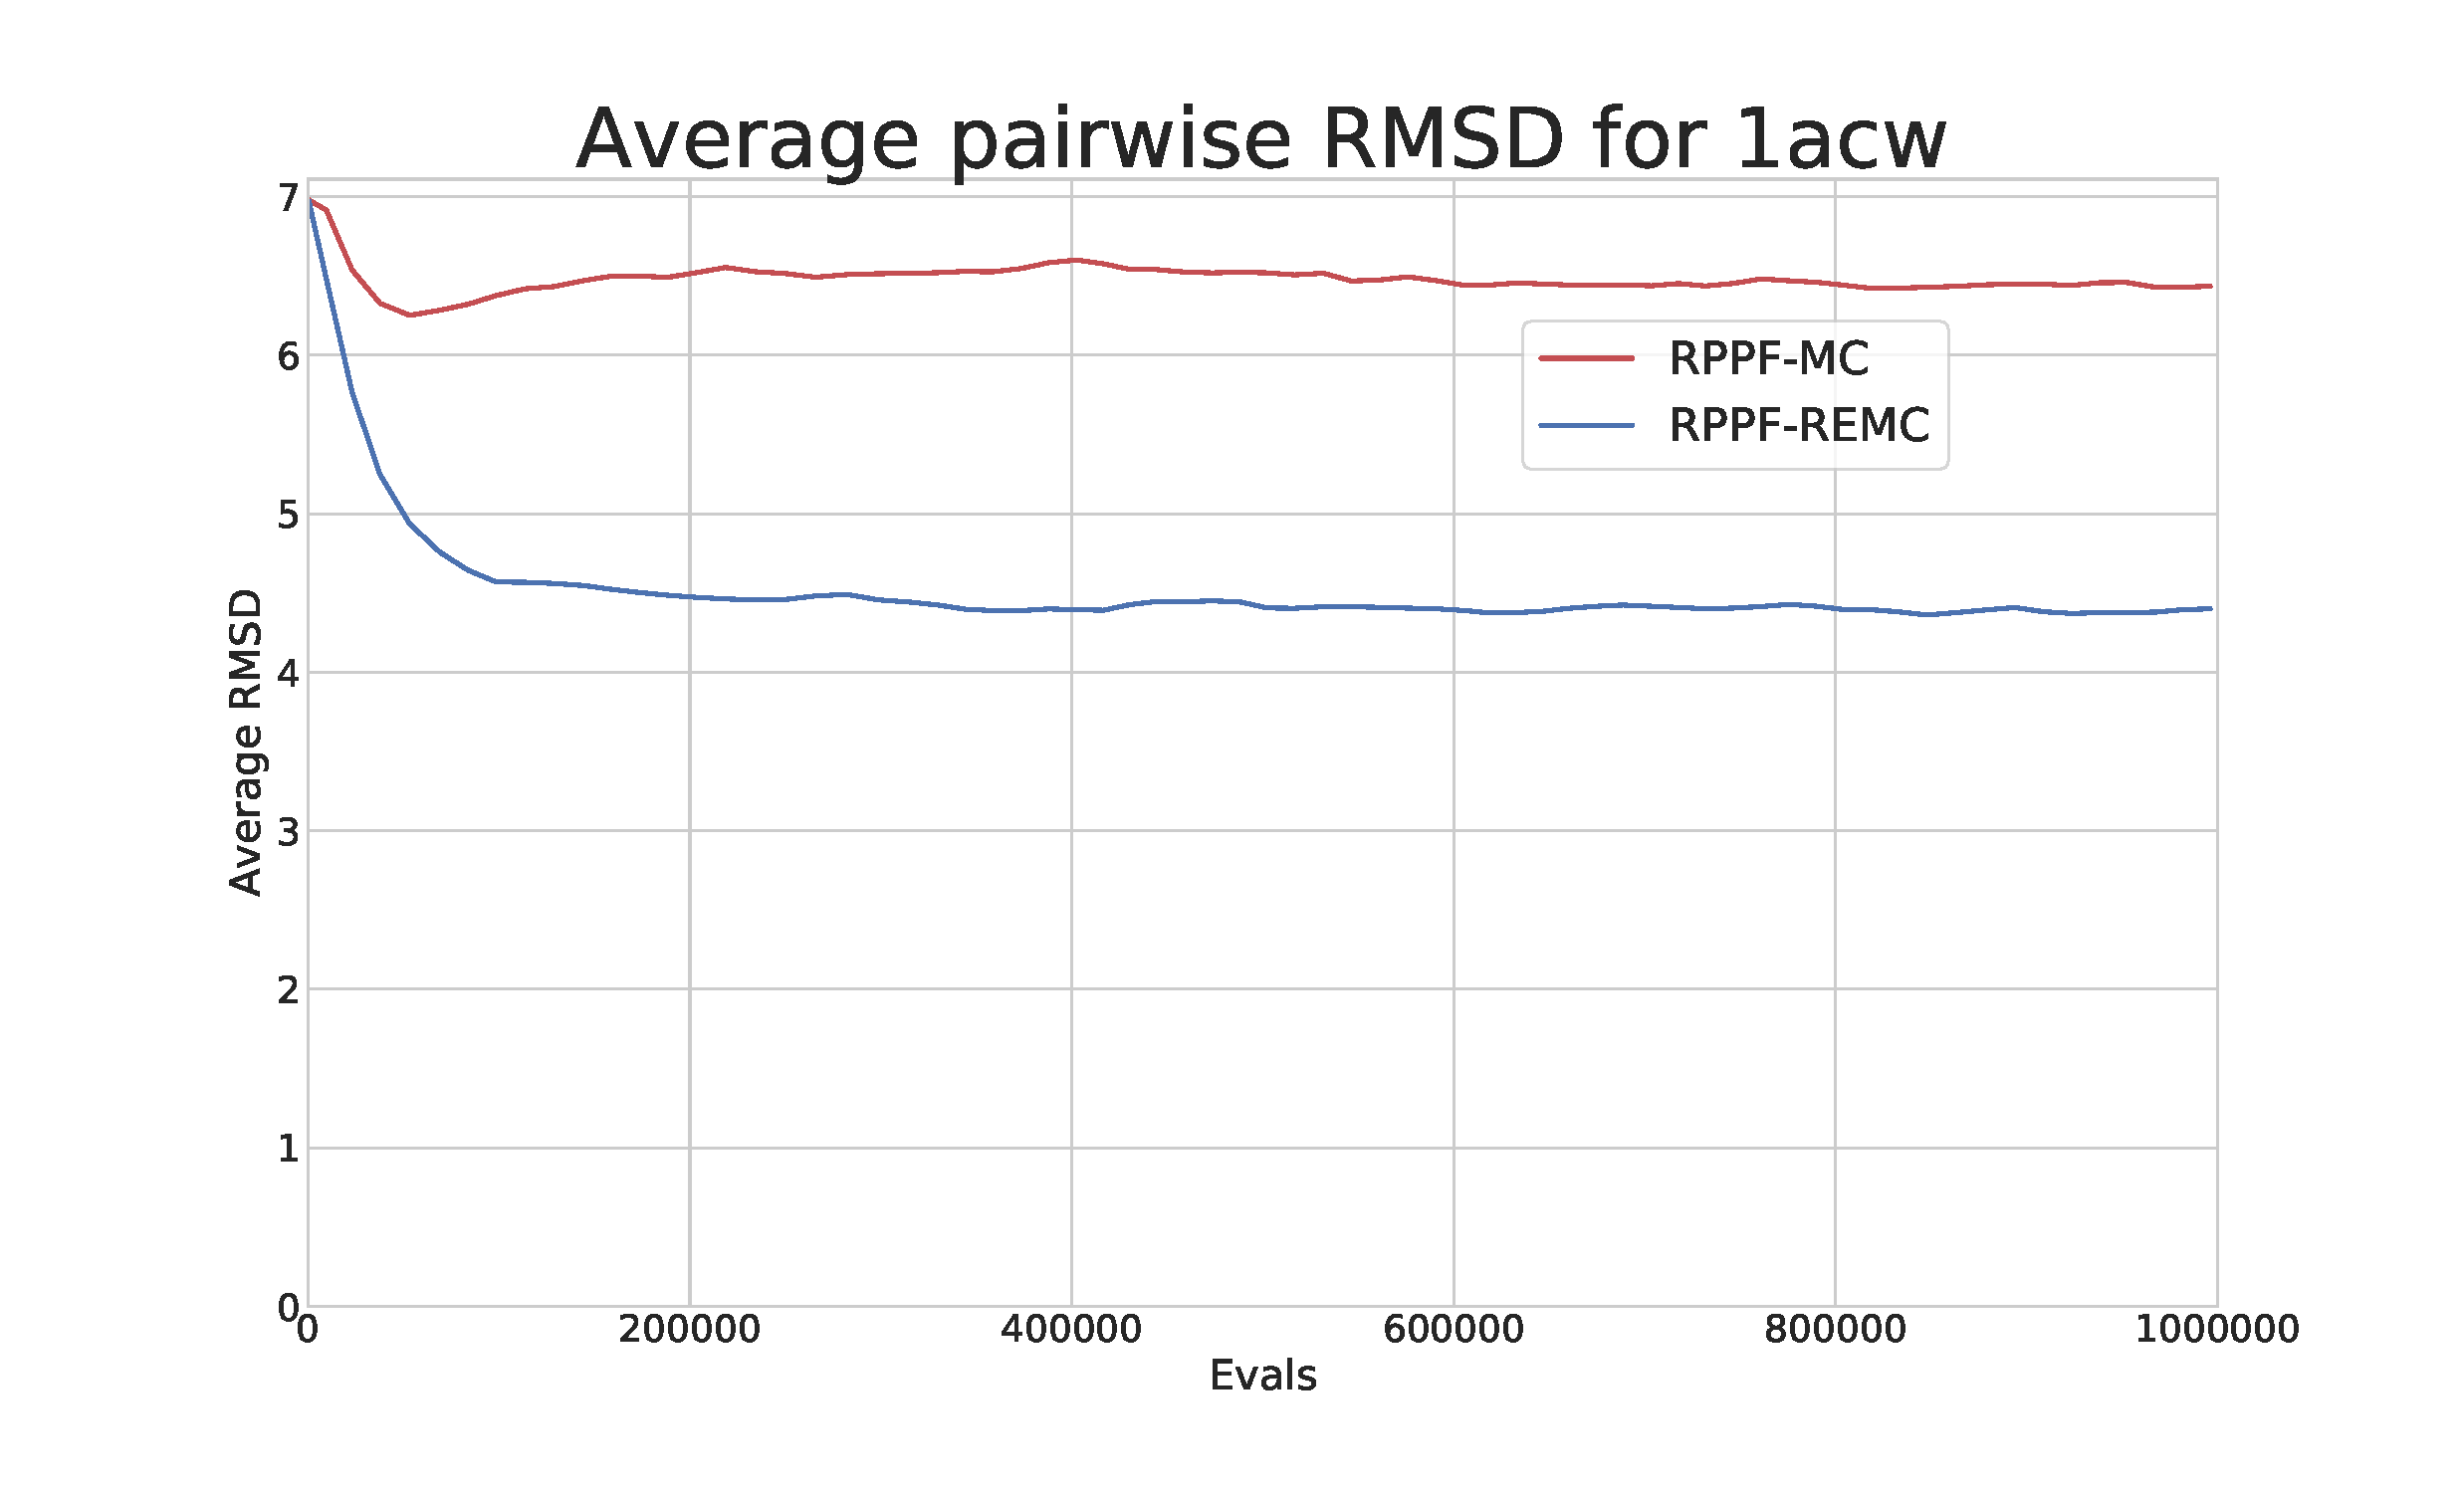
\includegraphics[width=1\linewidth]{Figuras/plots/rmsd_convergence/avg_rmsd_1acw.pdf}
    \caption{1acw}
    %\label{fig:1acw-conformation}
  \end{subfigure}
%
  \begin{subfigure}{0.7\linewidth}
    \centering
    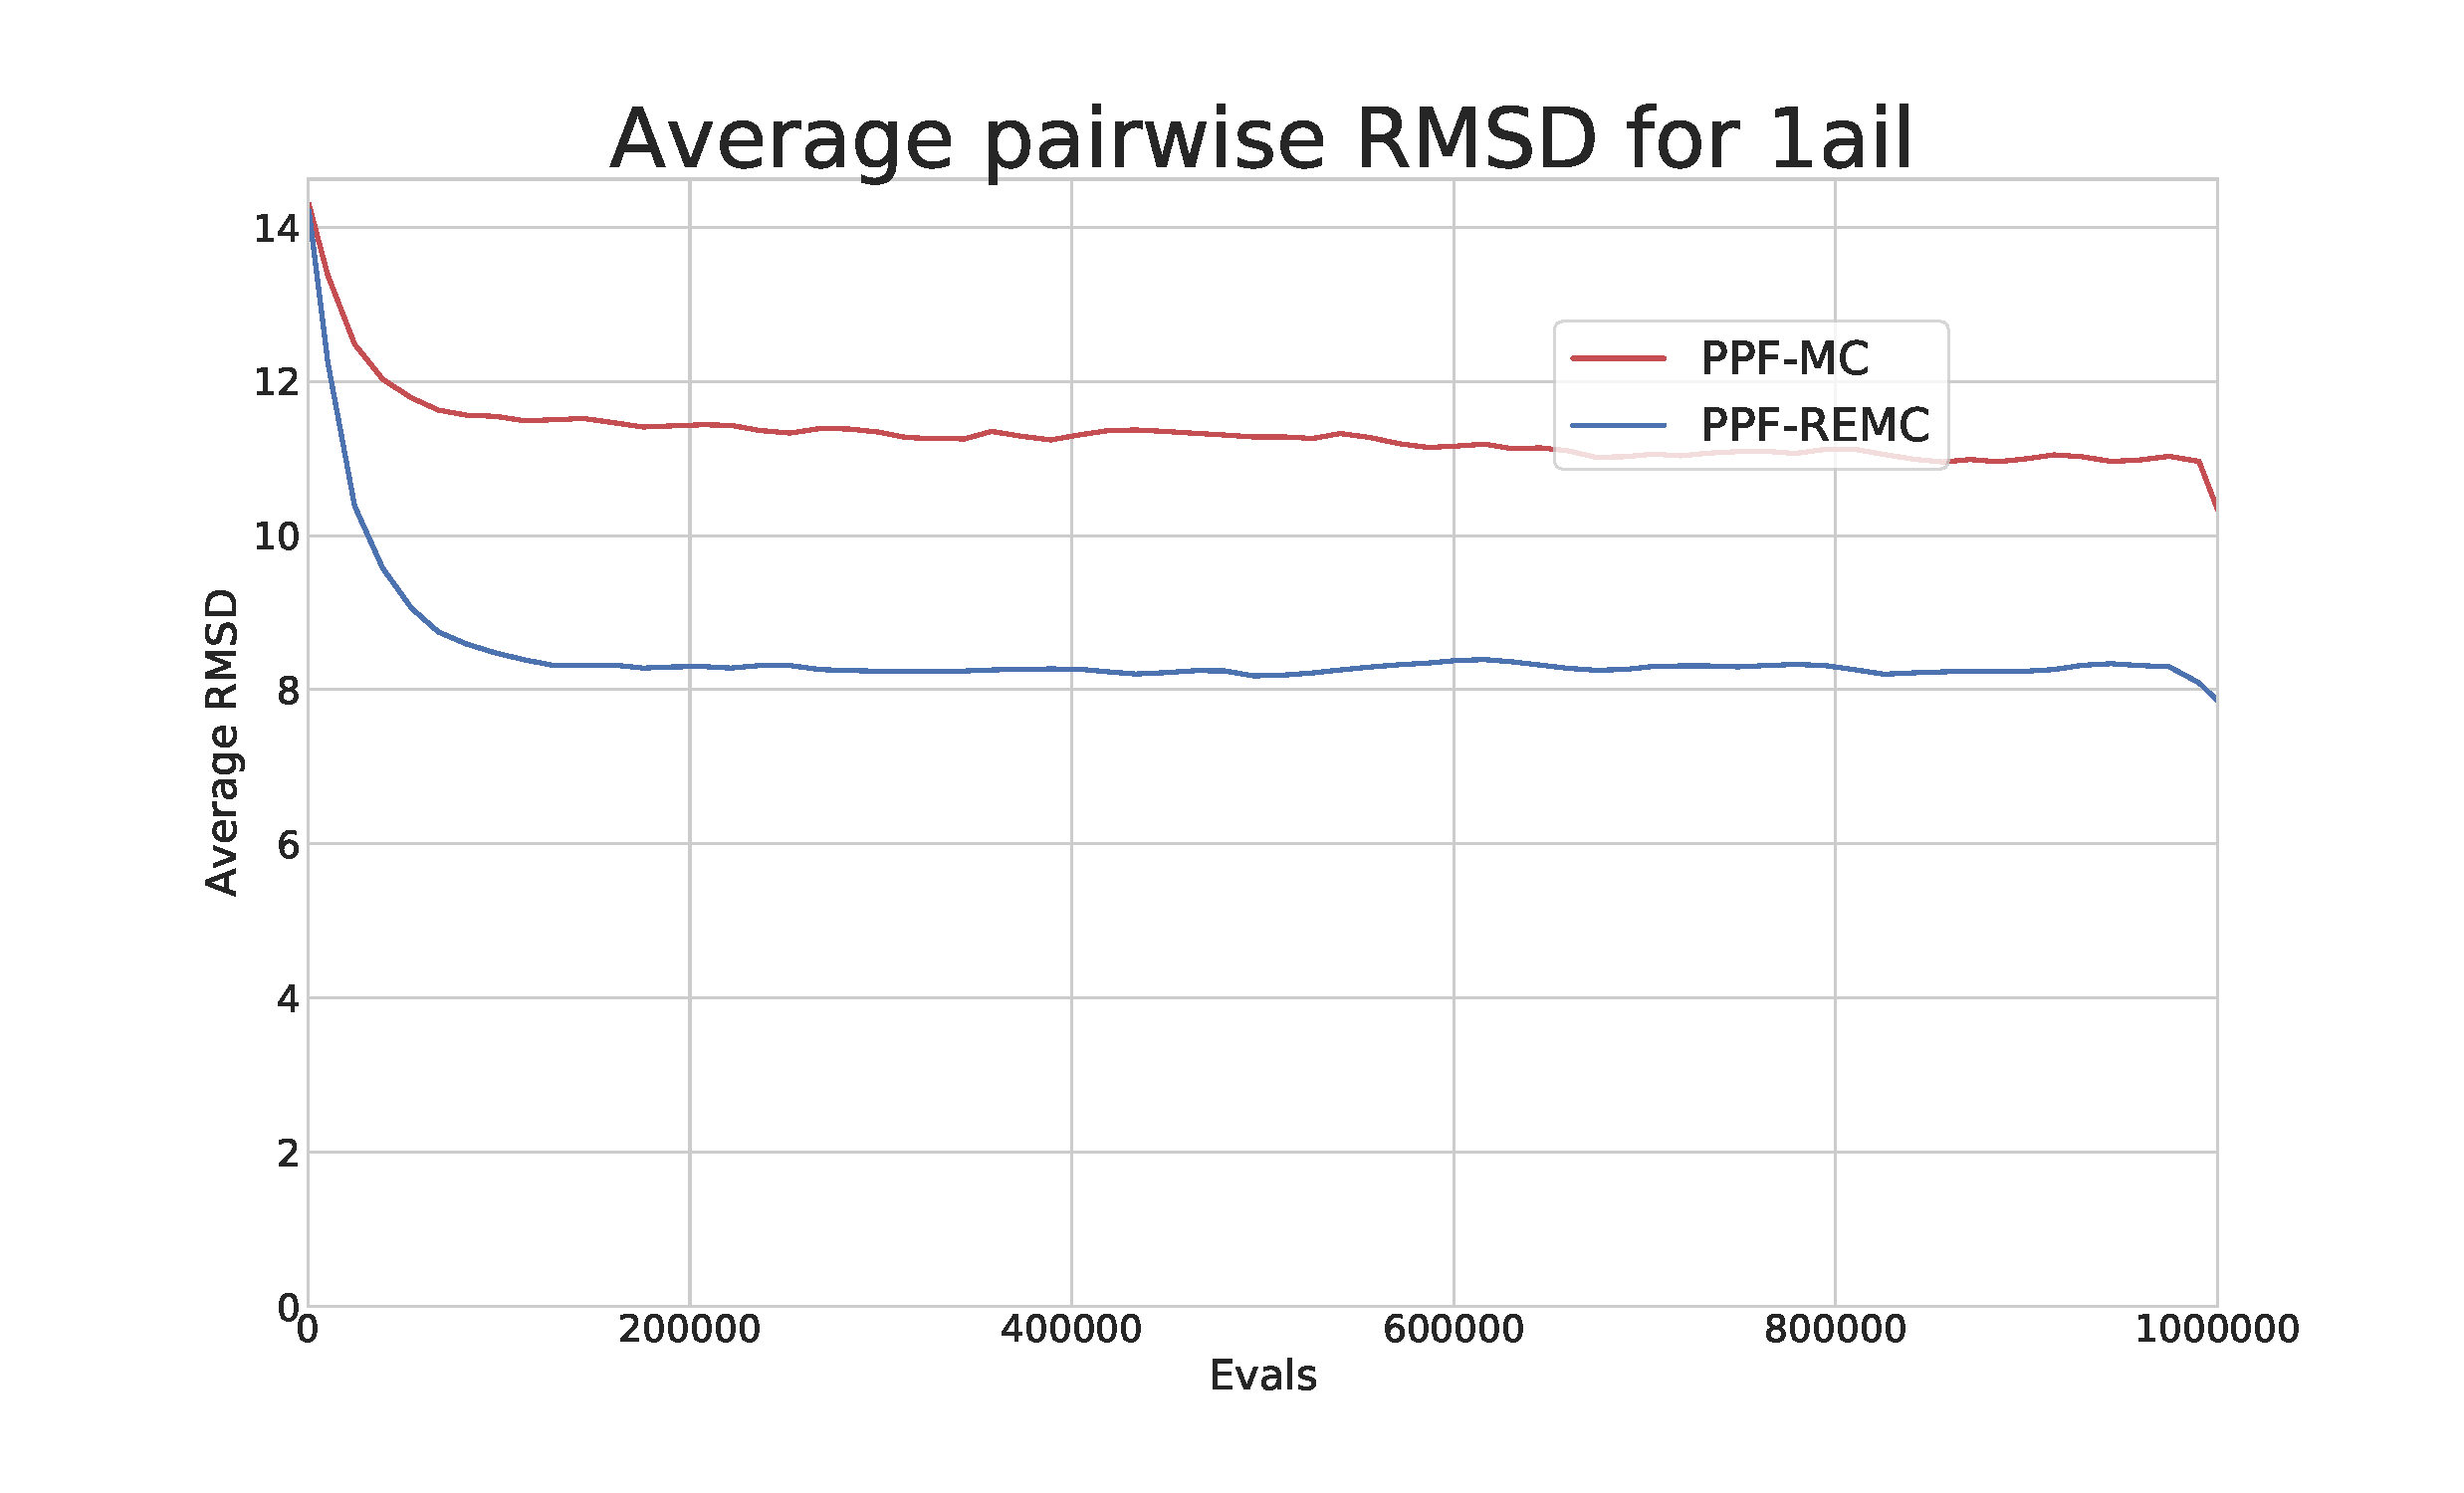
\includegraphics[width=1\linewidth]{Figuras/plots/rmsd_convergence/avg_rmsd_1ail.pdf}
    \caption{1ail}
    %\label{fig:1acw-conformation}
  \end{subfigure}
%
  \begin{subfigure}{0.7\linewidth}
    \centering
    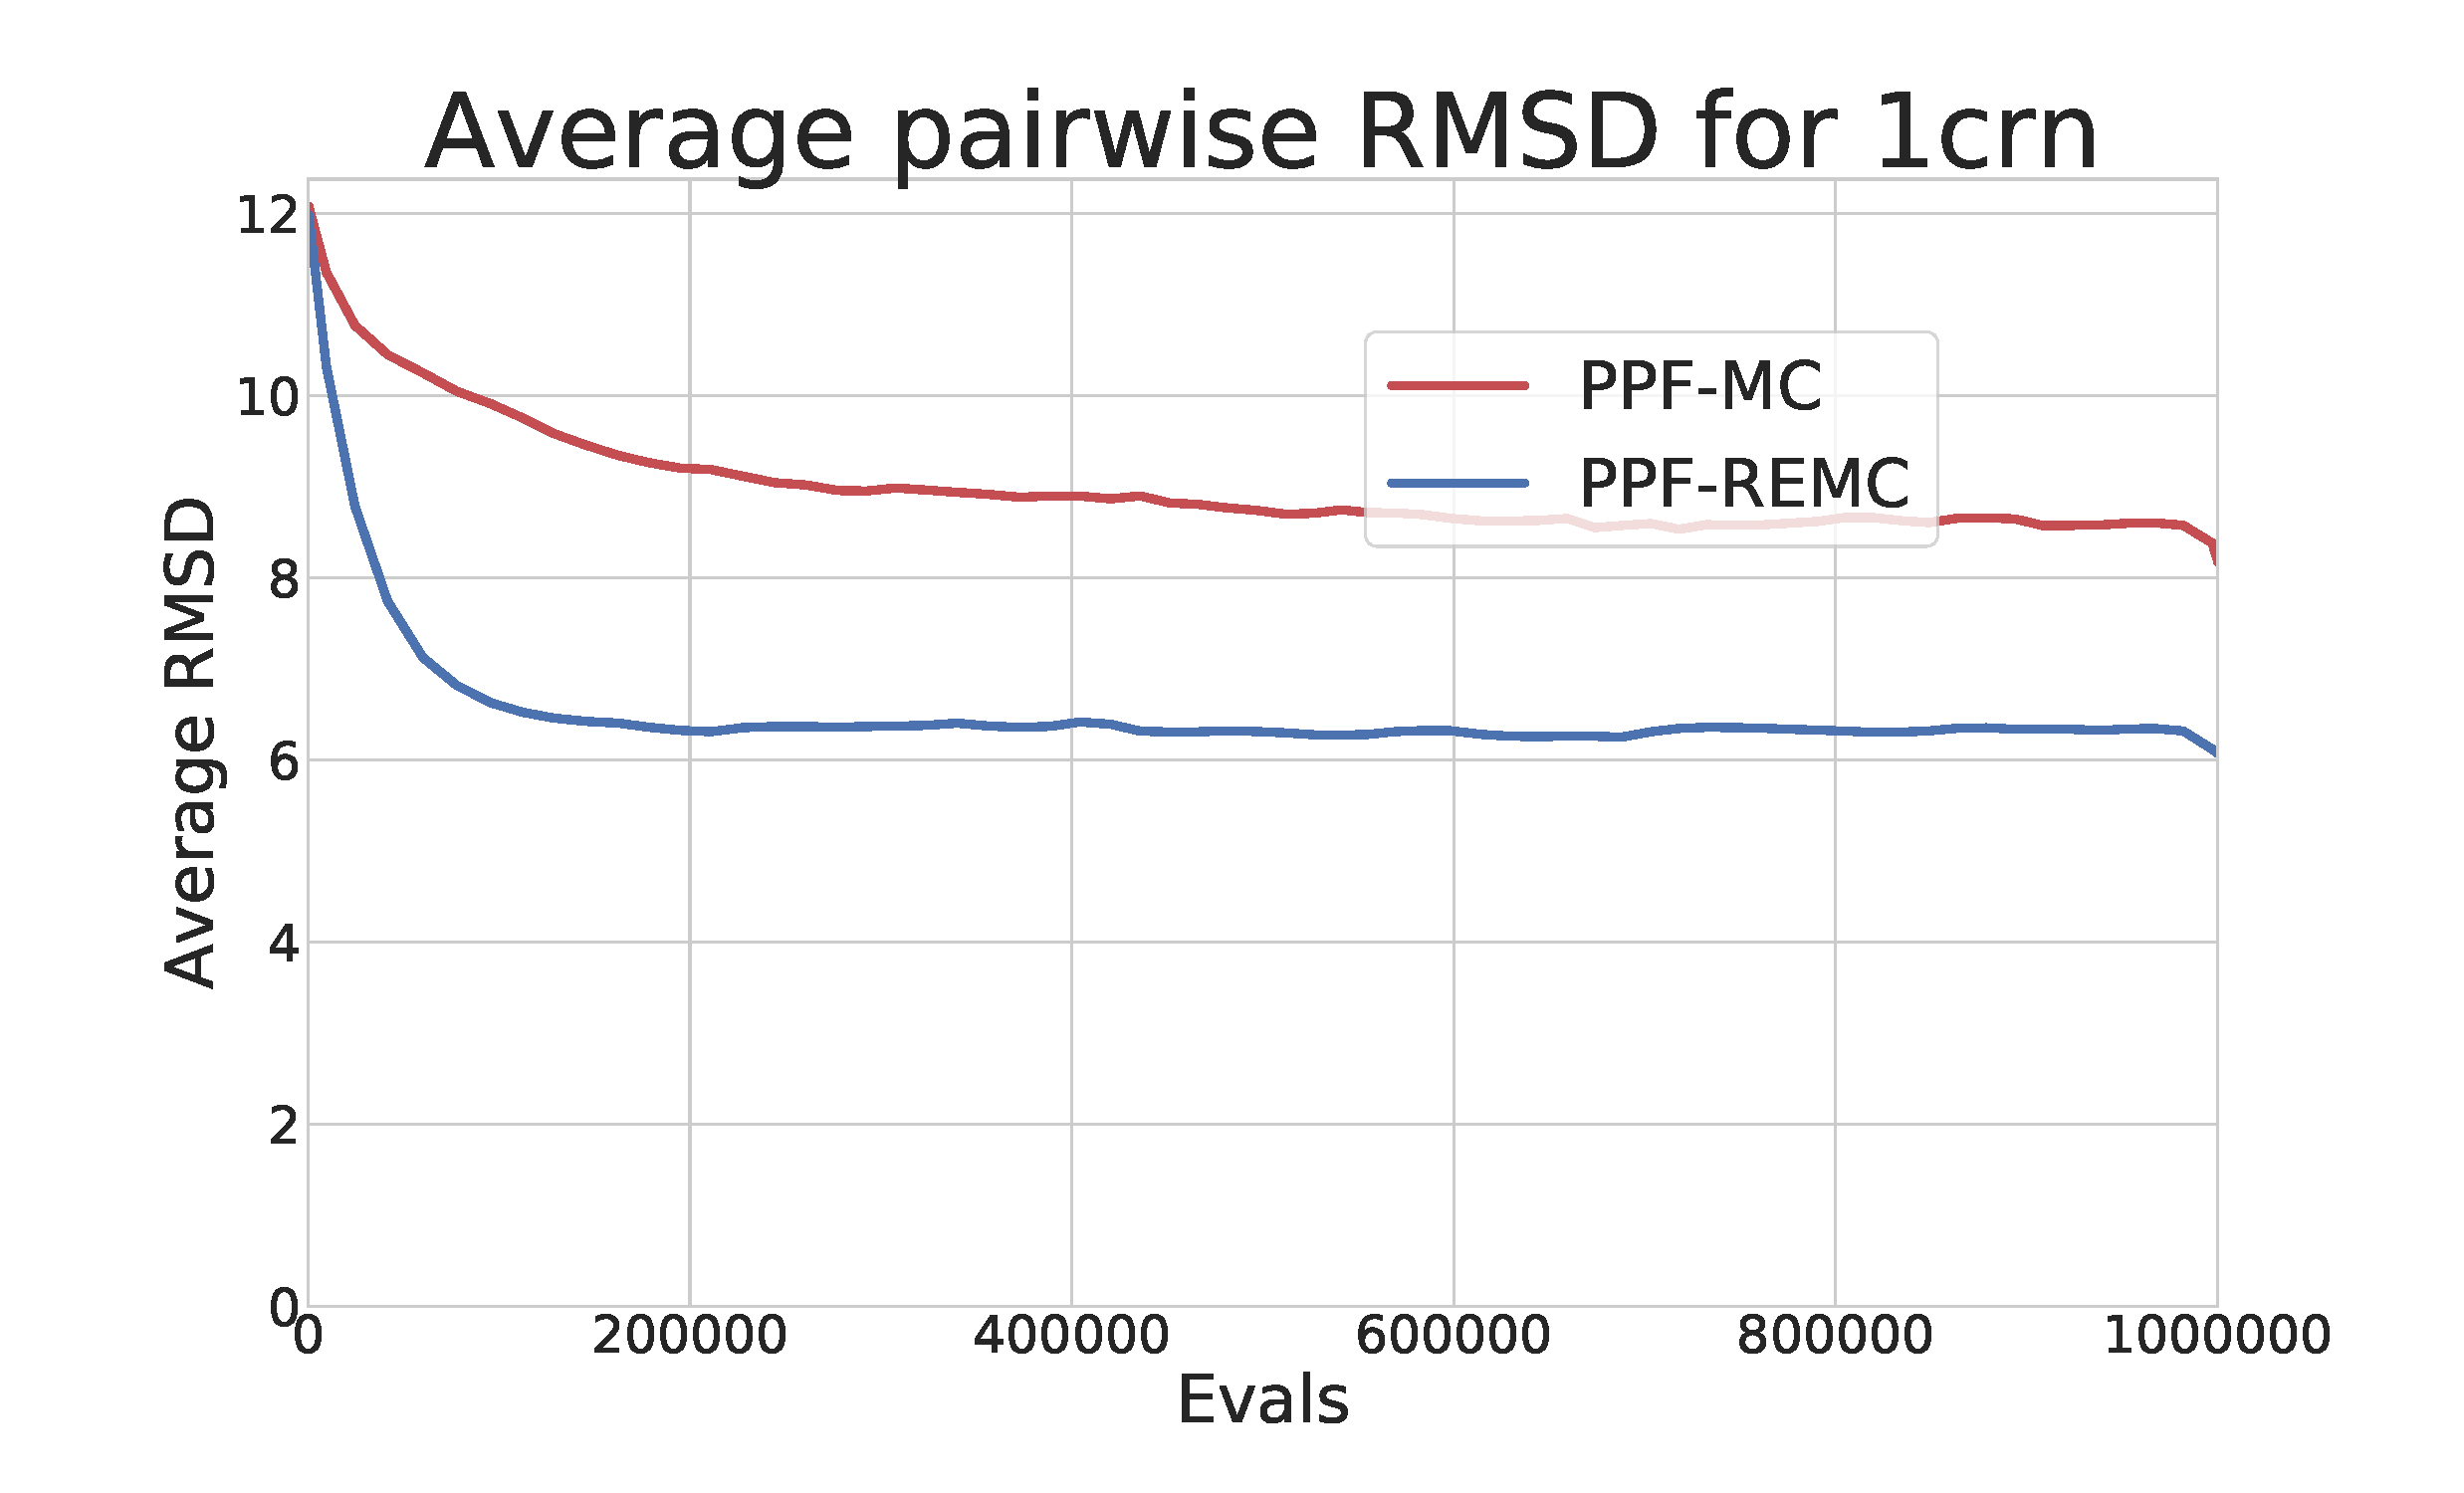
\includegraphics[width=1\linewidth]{Figuras/plots/rmsd_convergence/avg_rmsd_1crn.pdf}
    \caption{1crn}
    %\label{fig:1acw-conformation}
  \end{subfigure}
\end{figure}

\begin{figure}[ht]\ContinuedFloat
  \begin{subfigure}{0.7\linewidth}
    \centering
    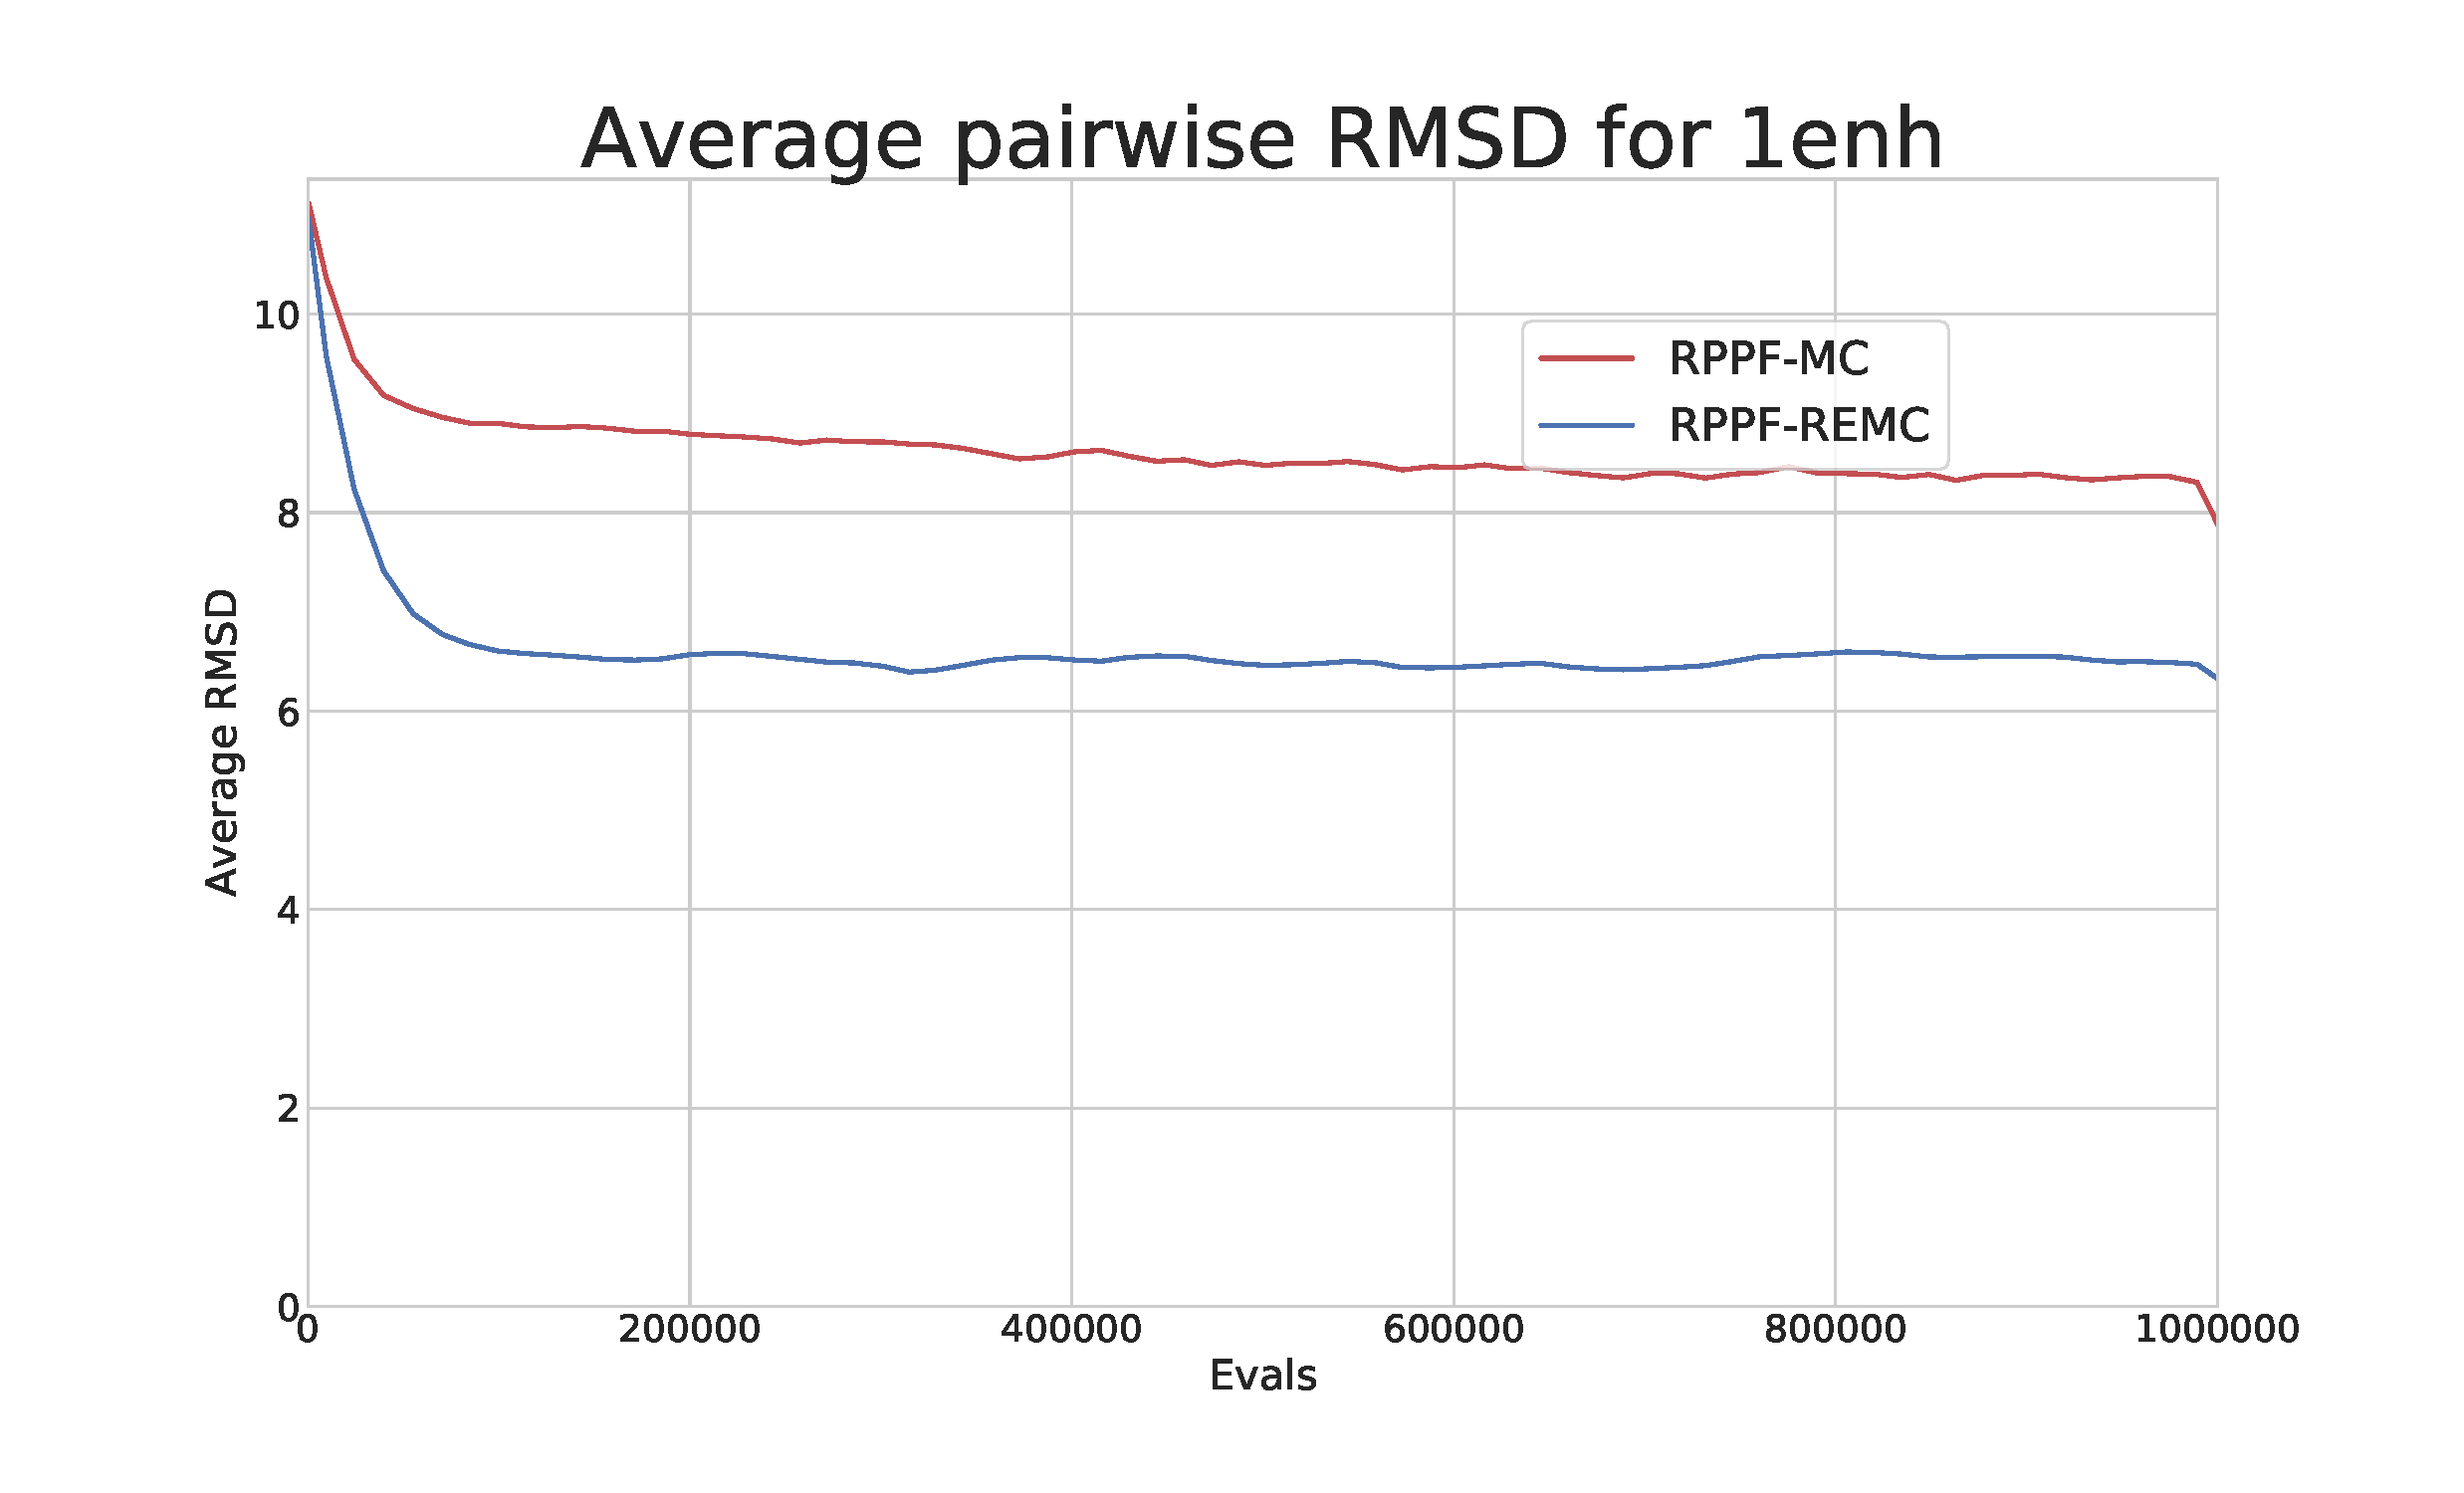
\includegraphics[width=1\linewidth]{Figuras/plots/rmsd_convergence/avg_rmsd_1enh.pdf}
    \caption{1enh}
    %\label{fig:1acw-conformation}
  \end{subfigure}
%
  \begin{subfigure}{0.7\linewidth}
    \centering
    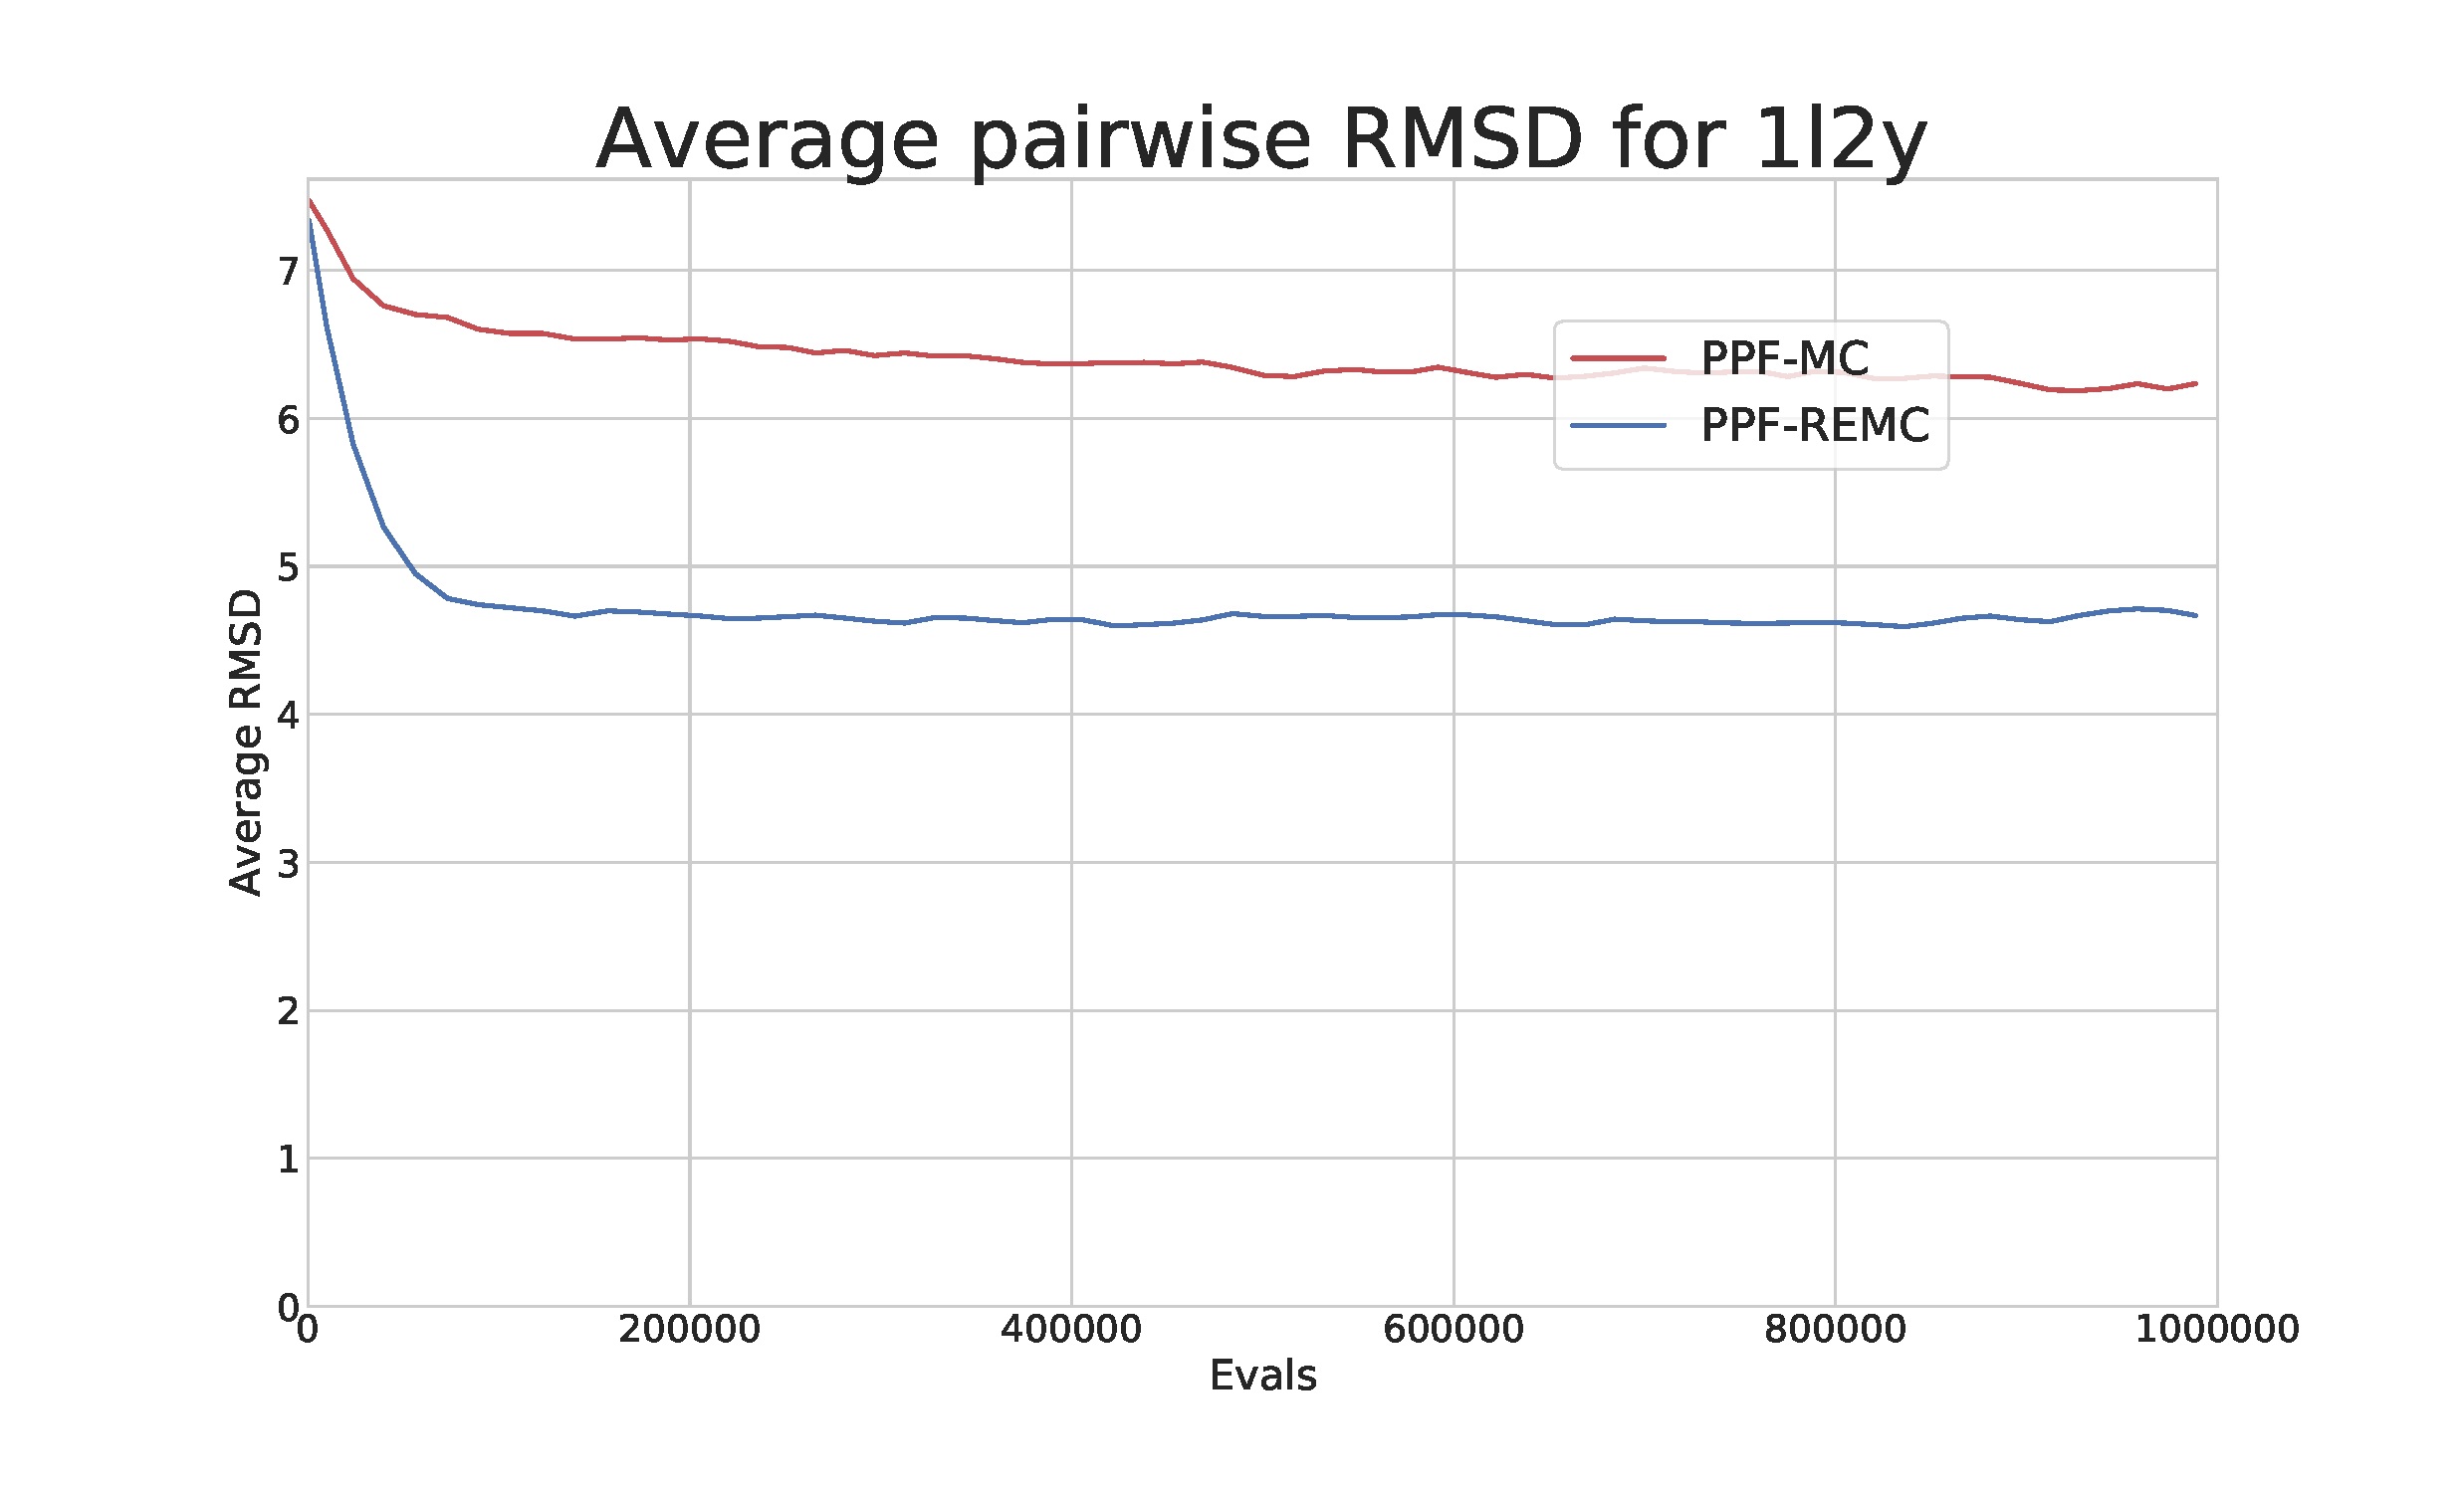
\includegraphics[width=1\linewidth]{Figuras/plots/rmsd_convergence/avg_rmsd_1l2y.pdf}
    \caption{1utg}
    %\label{fig:1acw-conformation}
  \end{subfigure}
%
  \begin{subfigure}{0.7\linewidth}
    \centering
    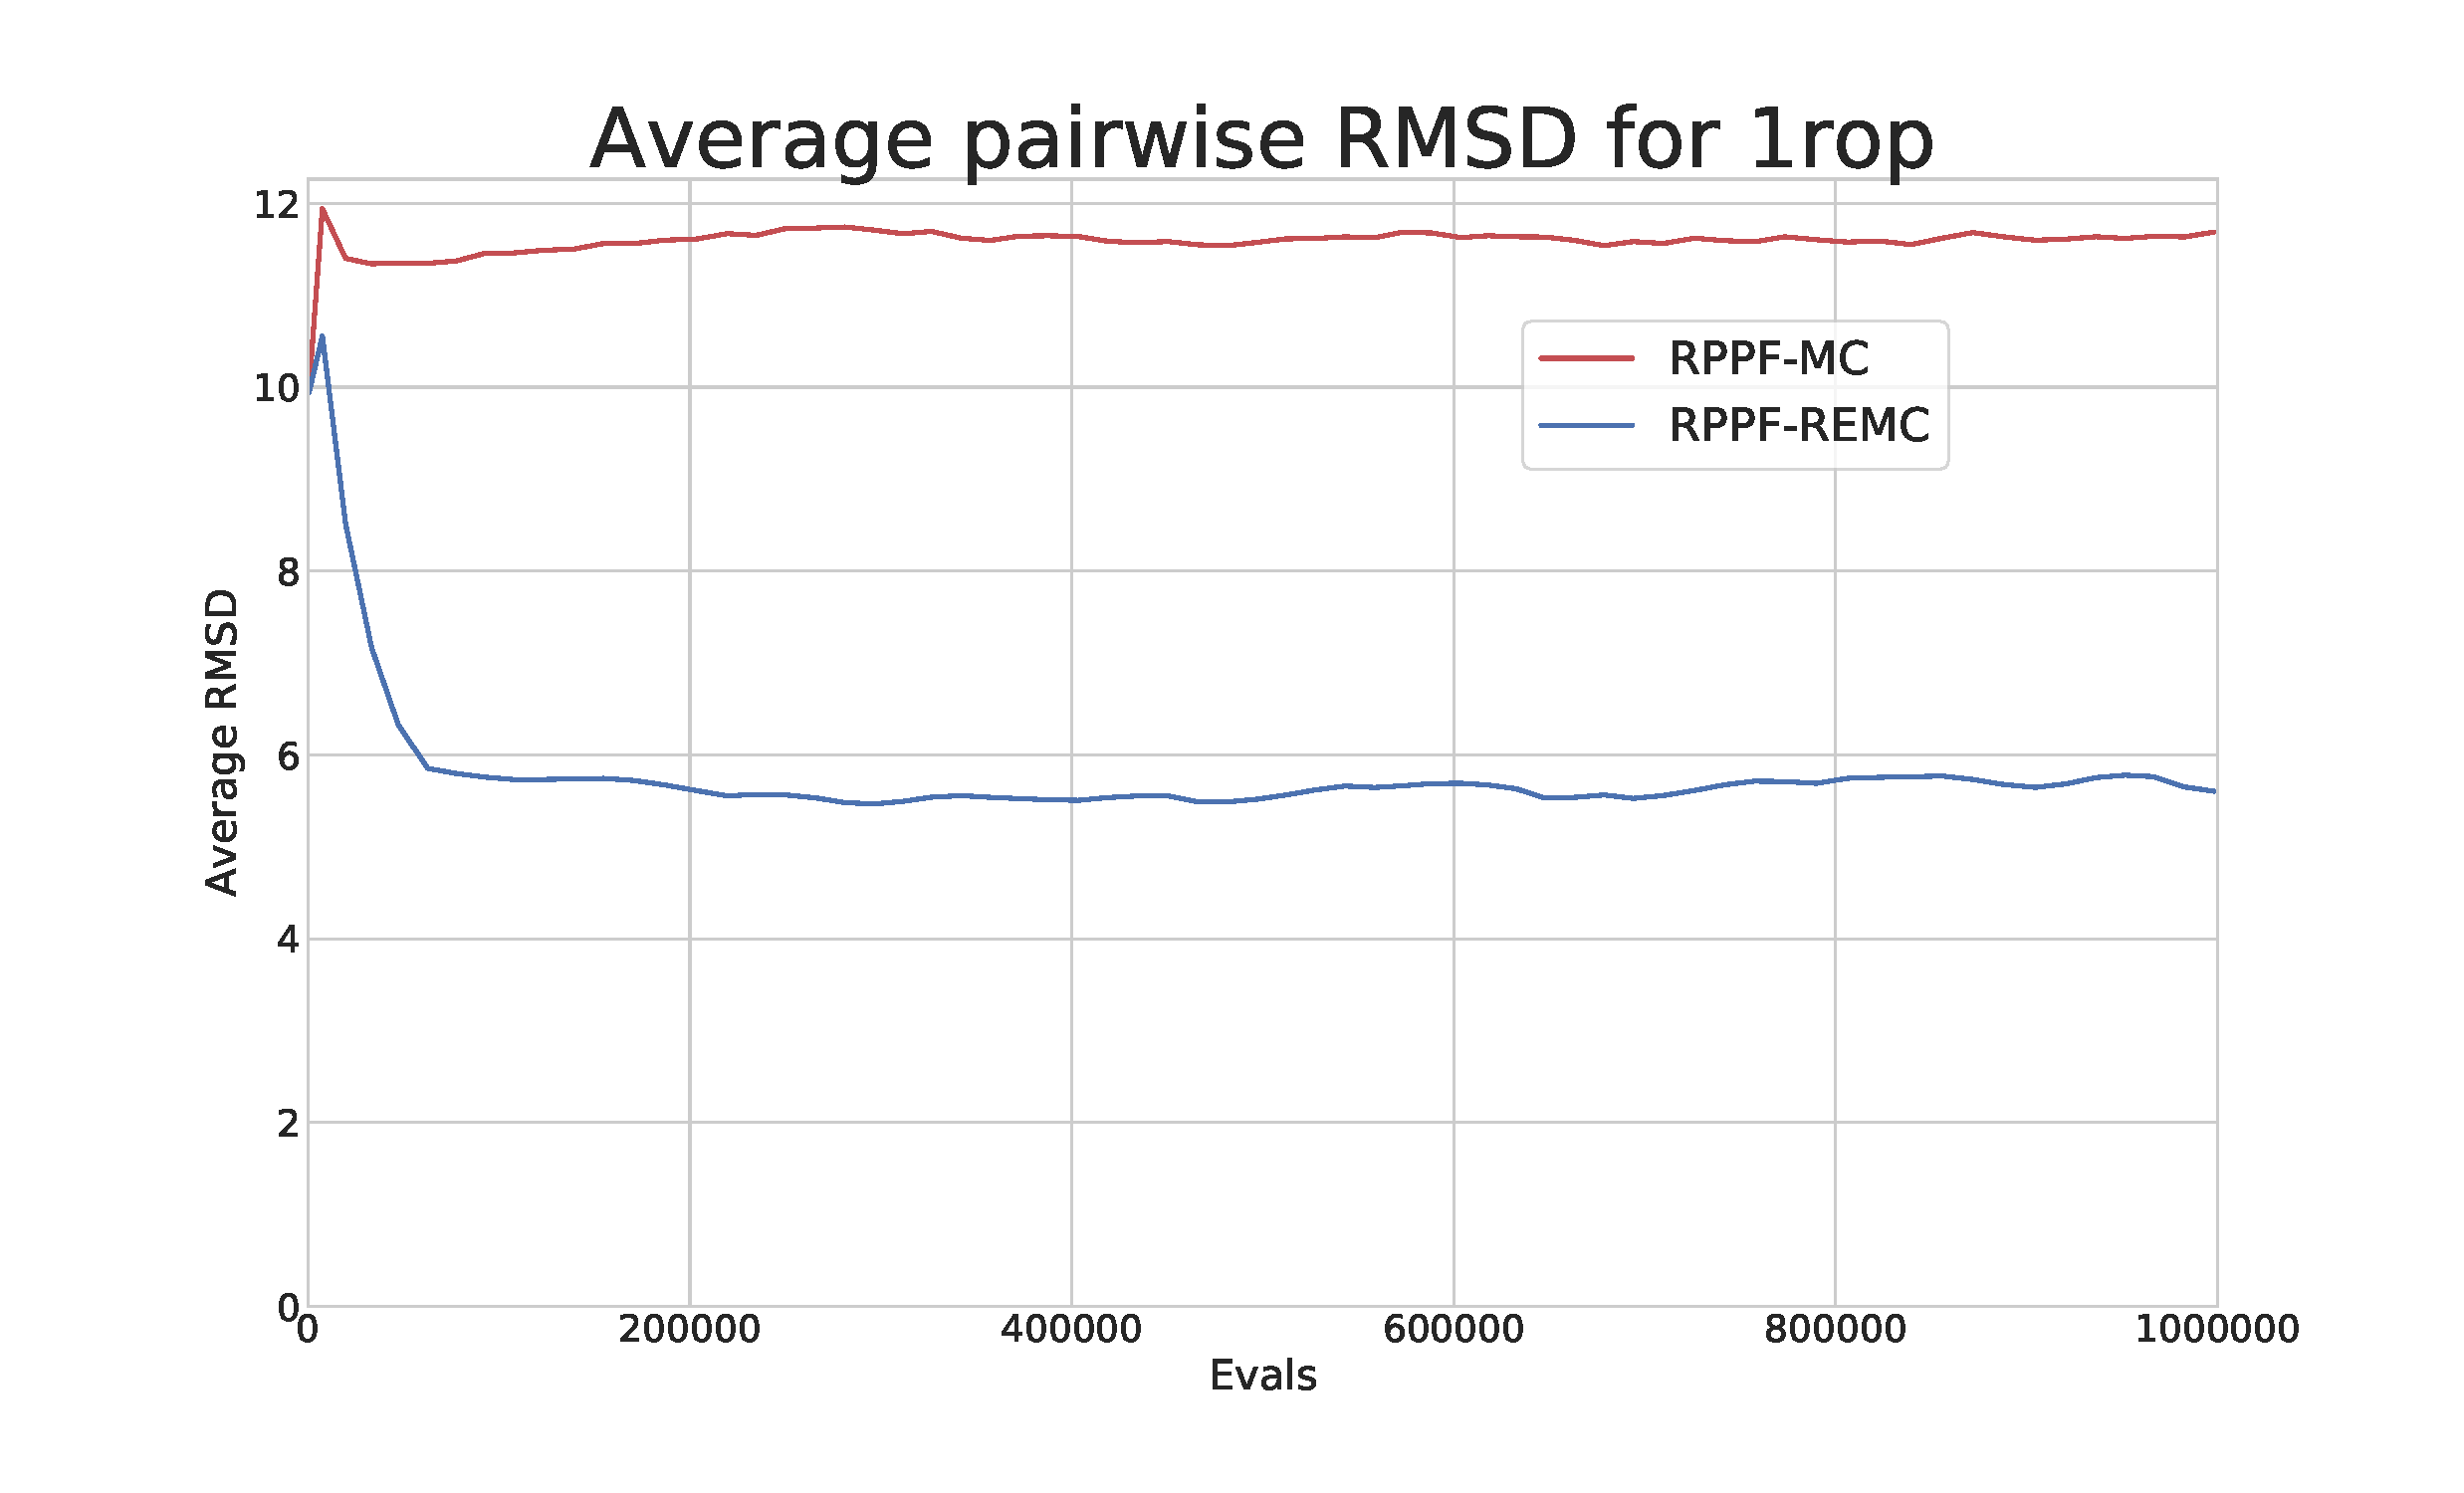
\includegraphics[width=1\linewidth]{Figuras/plots/rmsd_convergence/avg_rmsd_1rop.pdf}
    \caption{1rop}
    %\label{fig:1acw-conformation}
  \end{subfigure}
\end{figure}

\begin{figure}[ht]\ContinuedFloat
  \begin{subfigure}{0.7\linewidth}
    \centering
    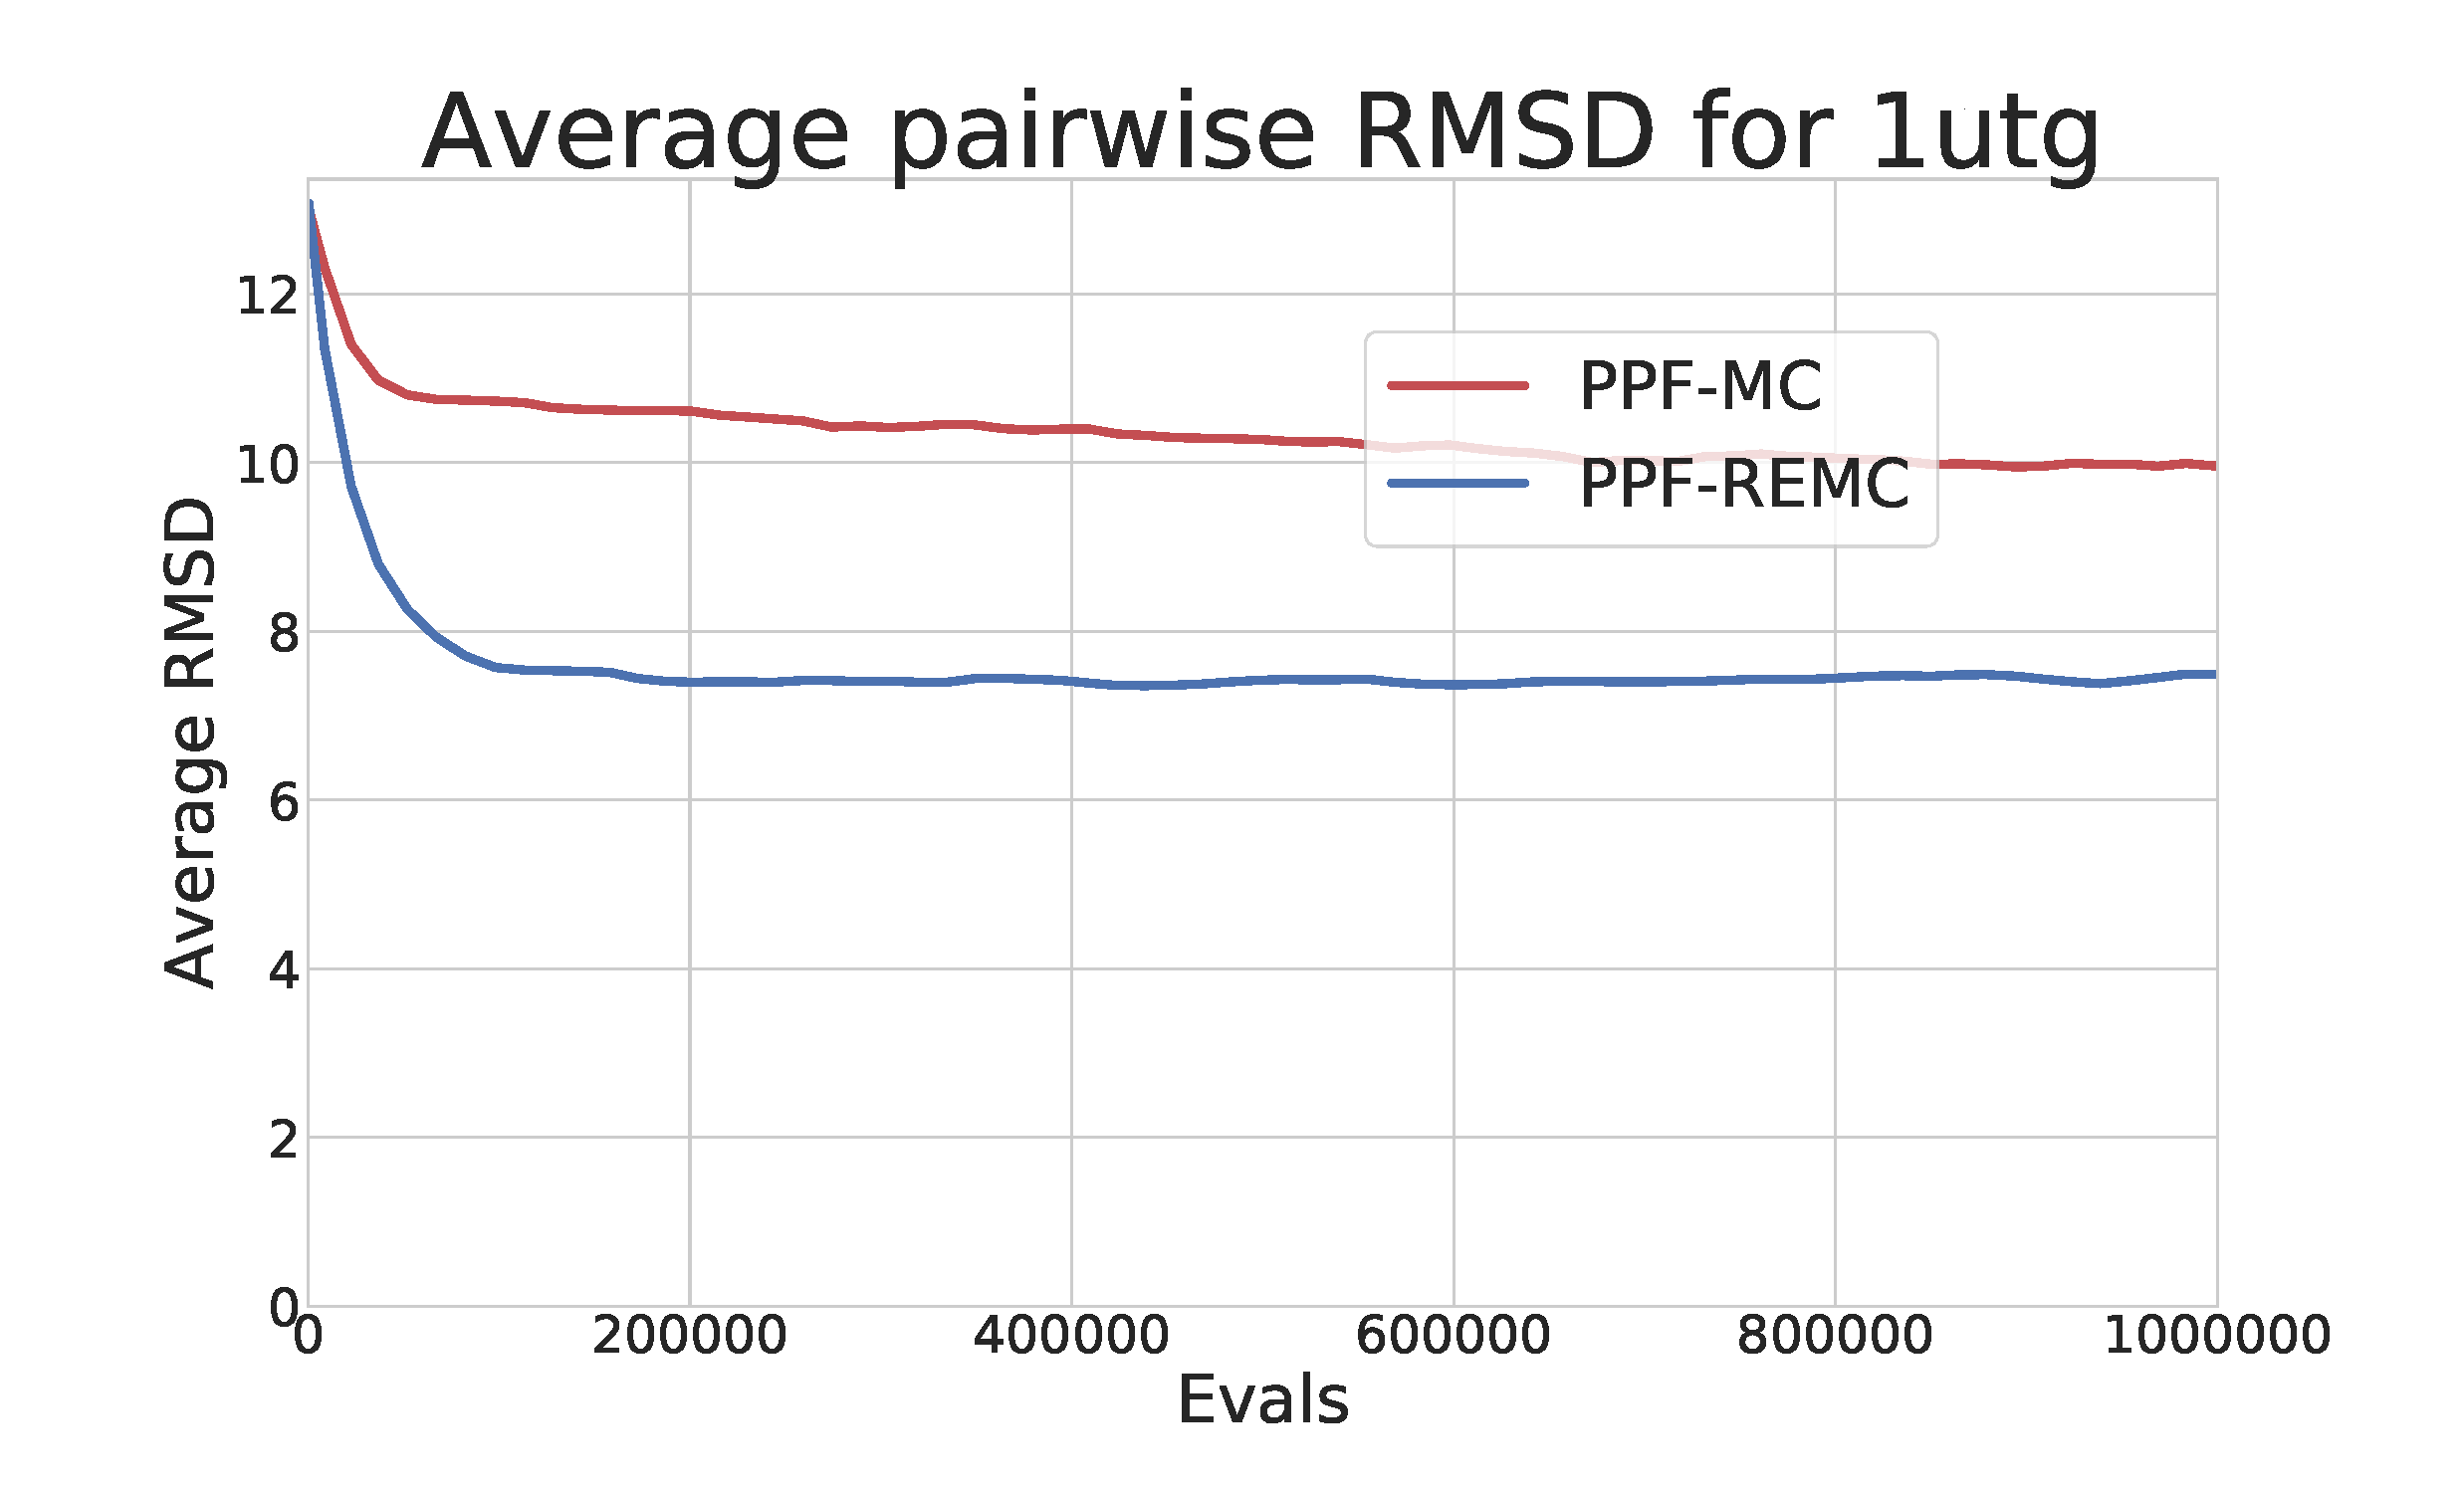
\includegraphics[width=1\linewidth]{Figuras/plots/rmsd_convergence/avg_rmsd_1utg.pdf}
    \caption{1utg}
    %\label{fig:1utg-conformation}
  \end{subfigure}
%
  \begin{subfigure}{0.7\linewidth}
    \centering
    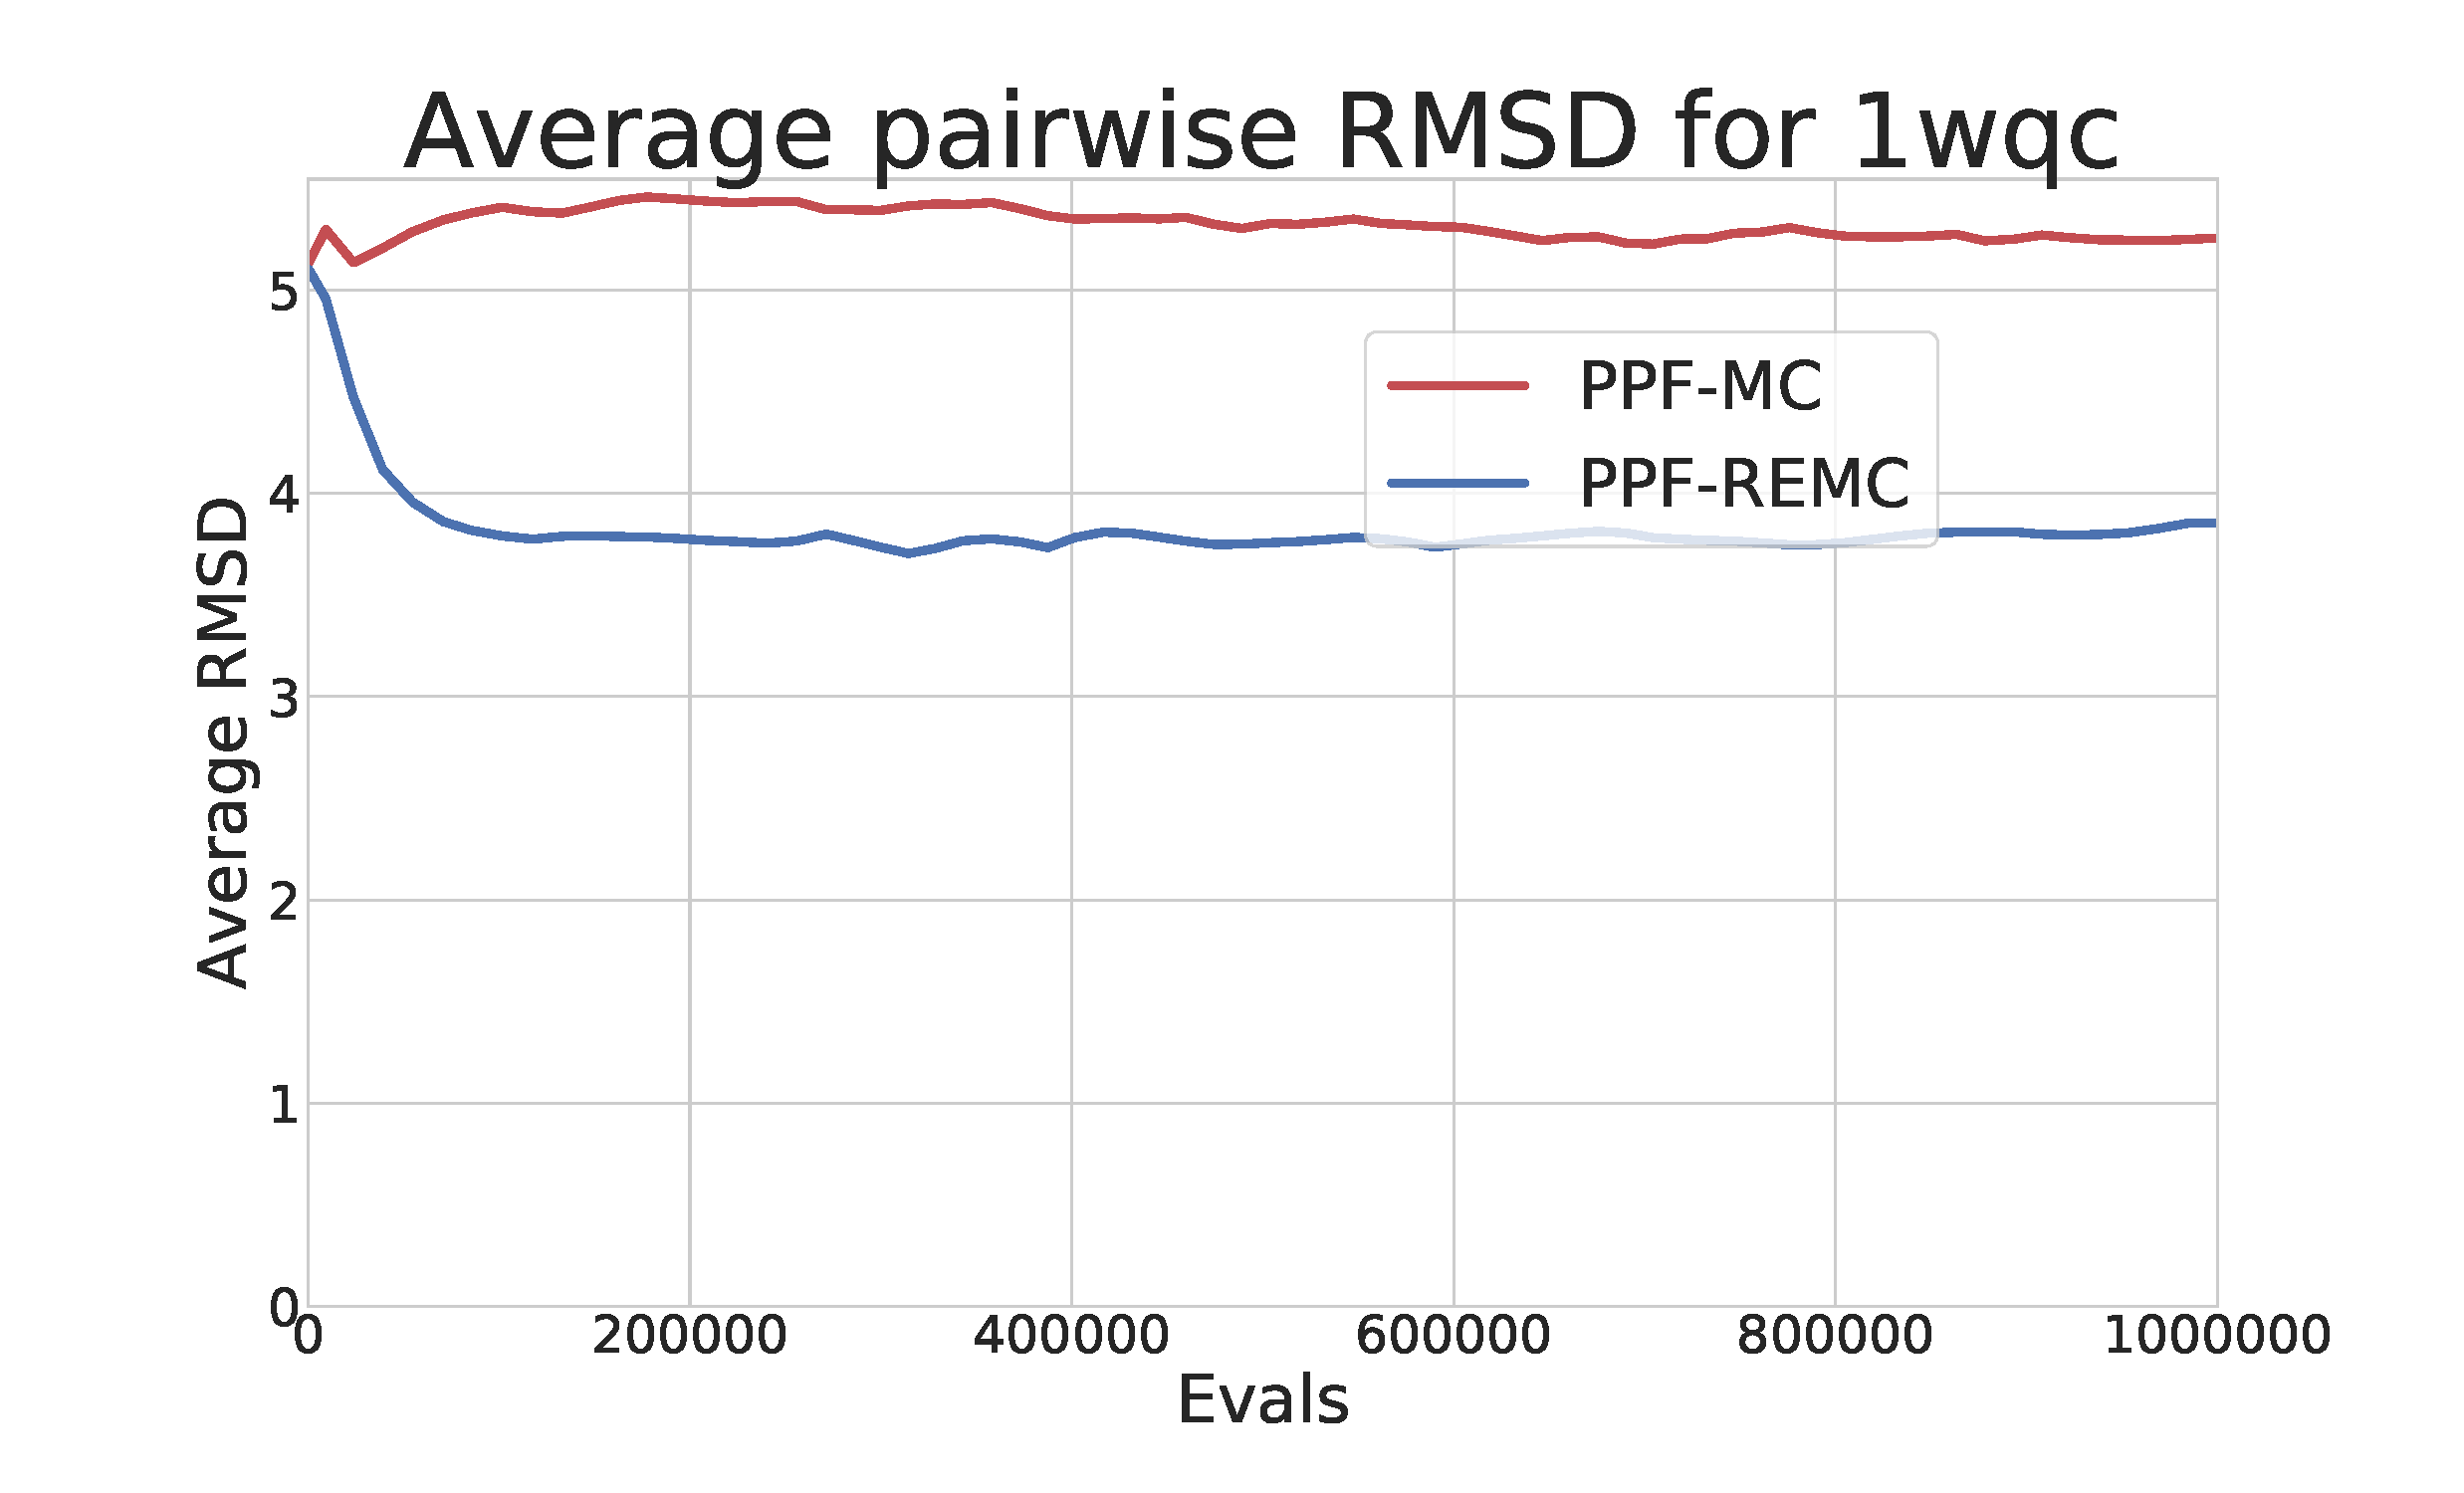
\includegraphics[width=1\linewidth]{Figuras/plots/rmsd_convergence/avg_rmsd_1wqc.pdf}
    \caption{1wqc}
    %\label{fig:1wqc-conformation}
  \end{subfigure}
%
  \begin{subfigure}{0.7\linewidth}
    \centering
    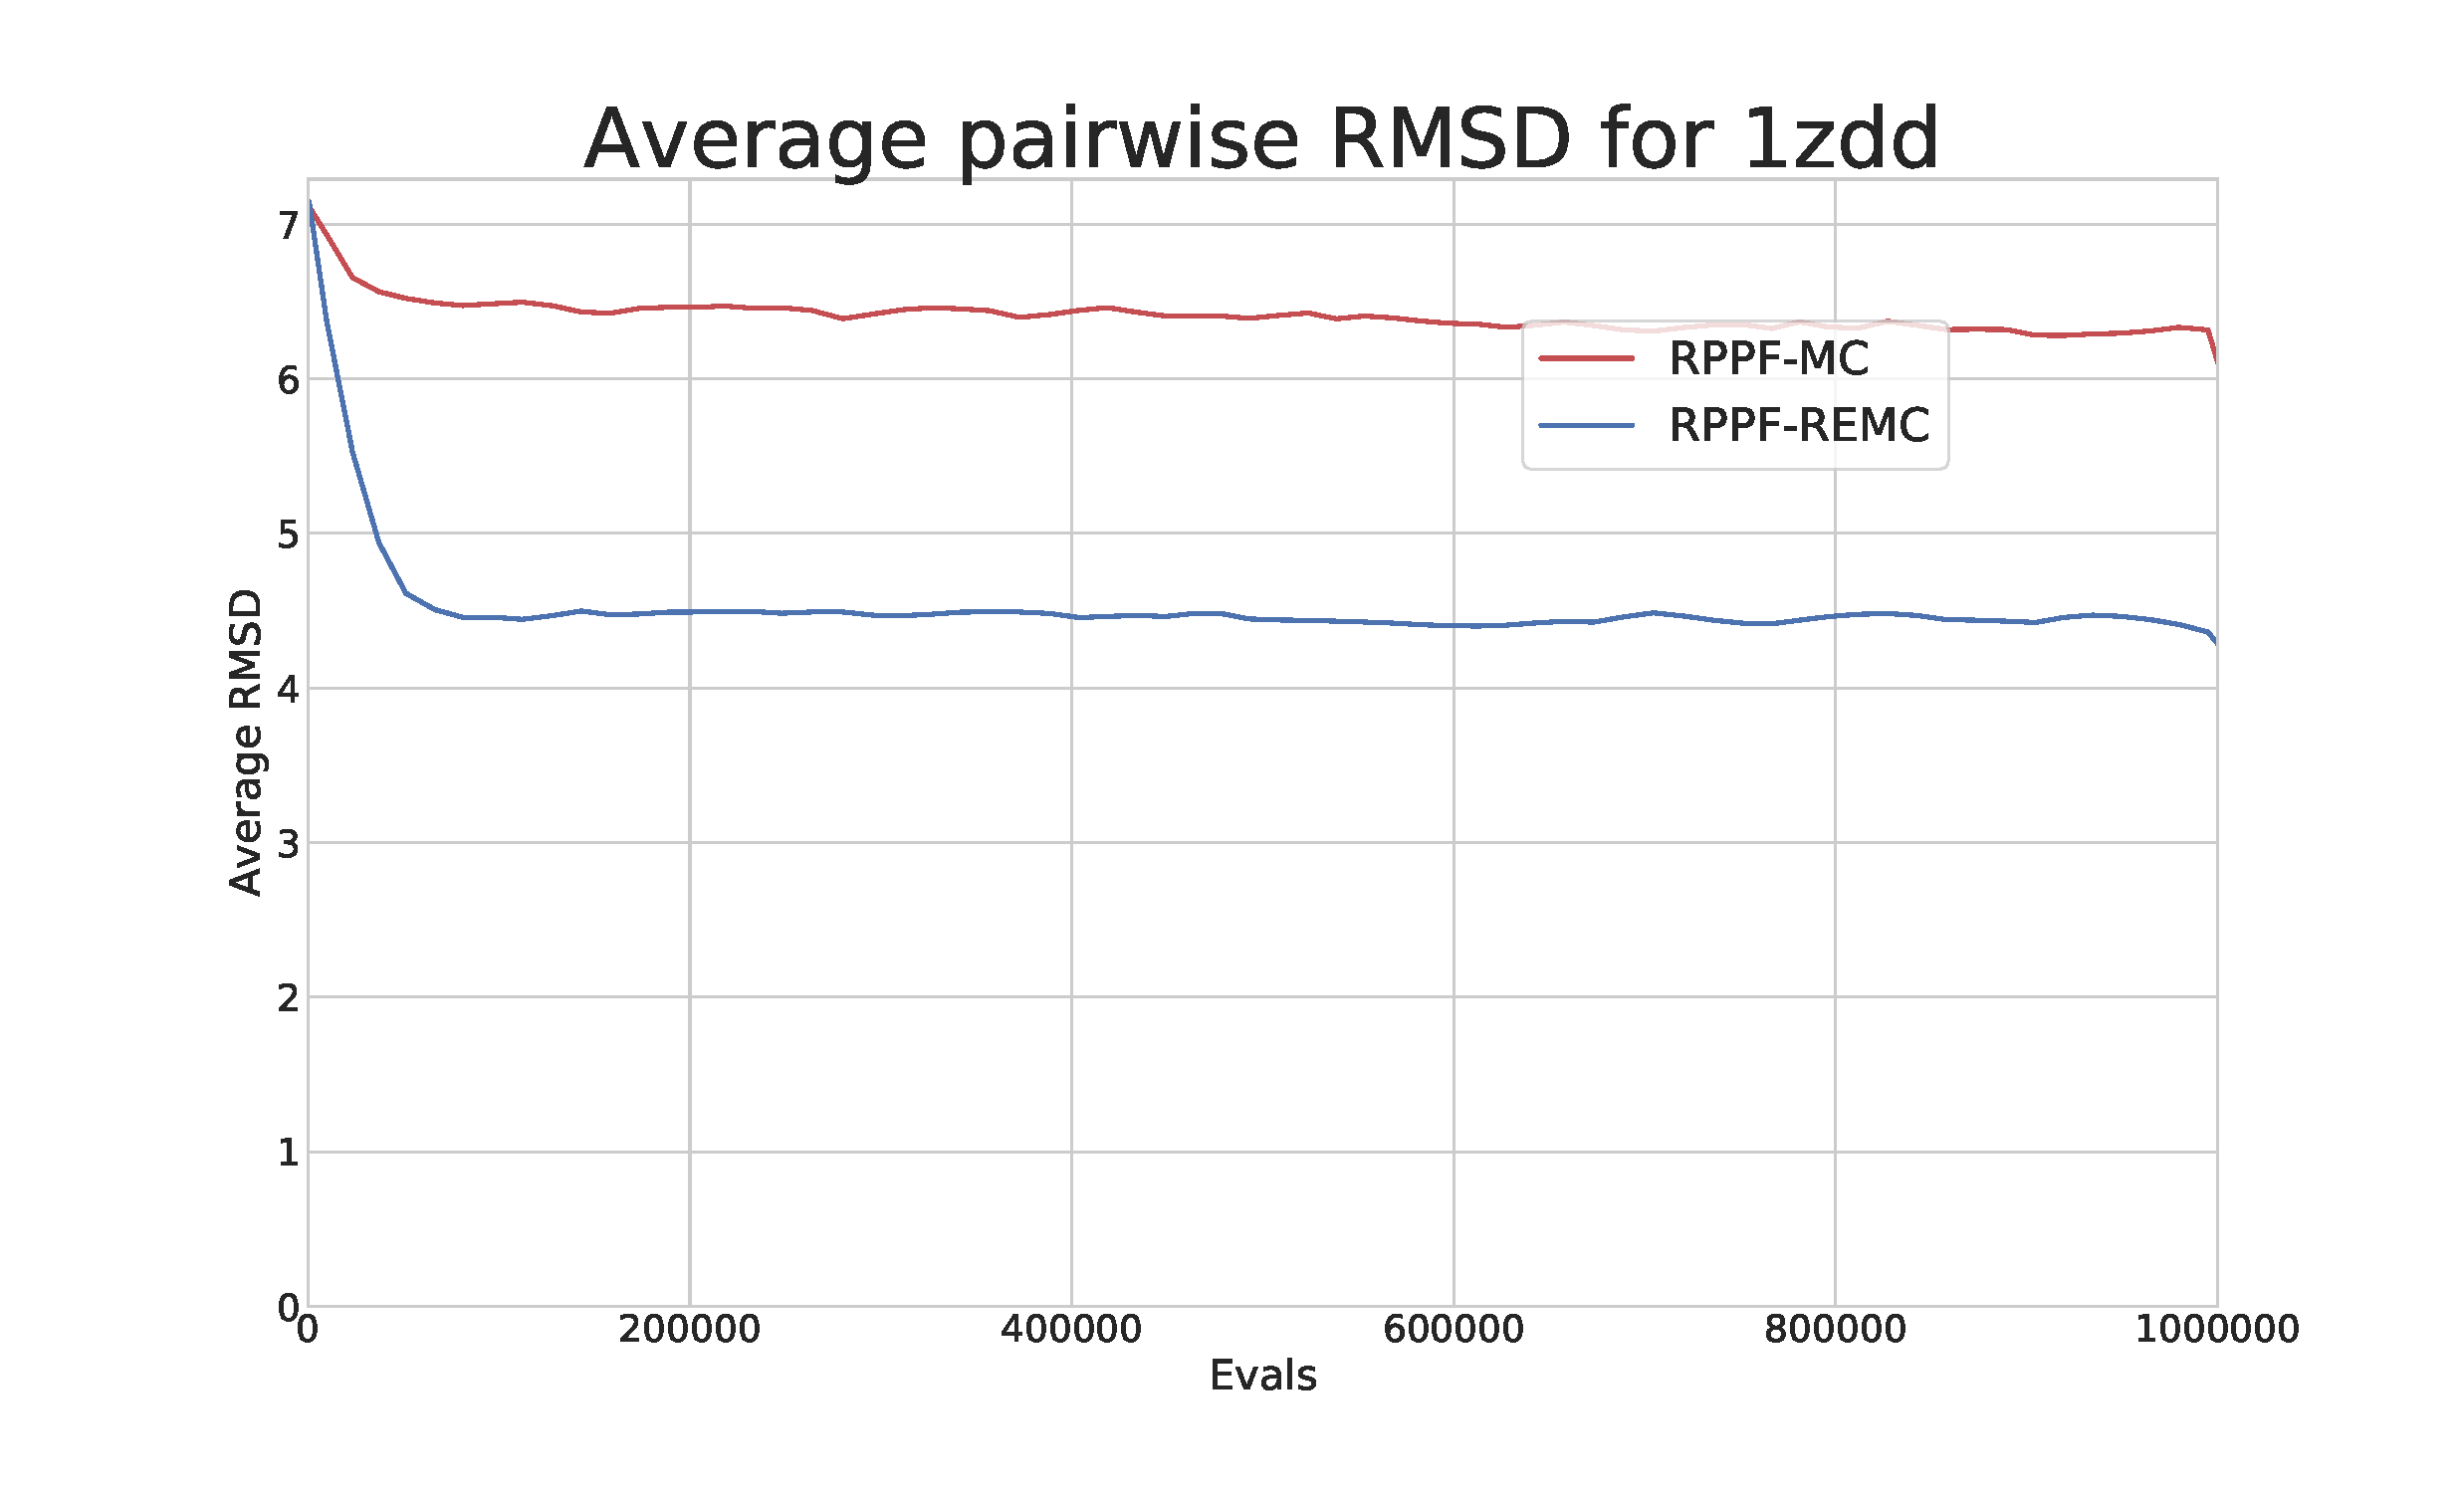
\includegraphics[width=1\linewidth]{Figuras/plots/rmsd_convergence/avg_rmsd_1zdd.pdf}
    \caption{1zdd}
    %\label{fig:1zdd-conformation}
  \end{subfigure}
\end{figure}

\begin{figure}[ht]\ContinuedFloat
  \begin{subfigure}{0.7\linewidth}
    \centering
    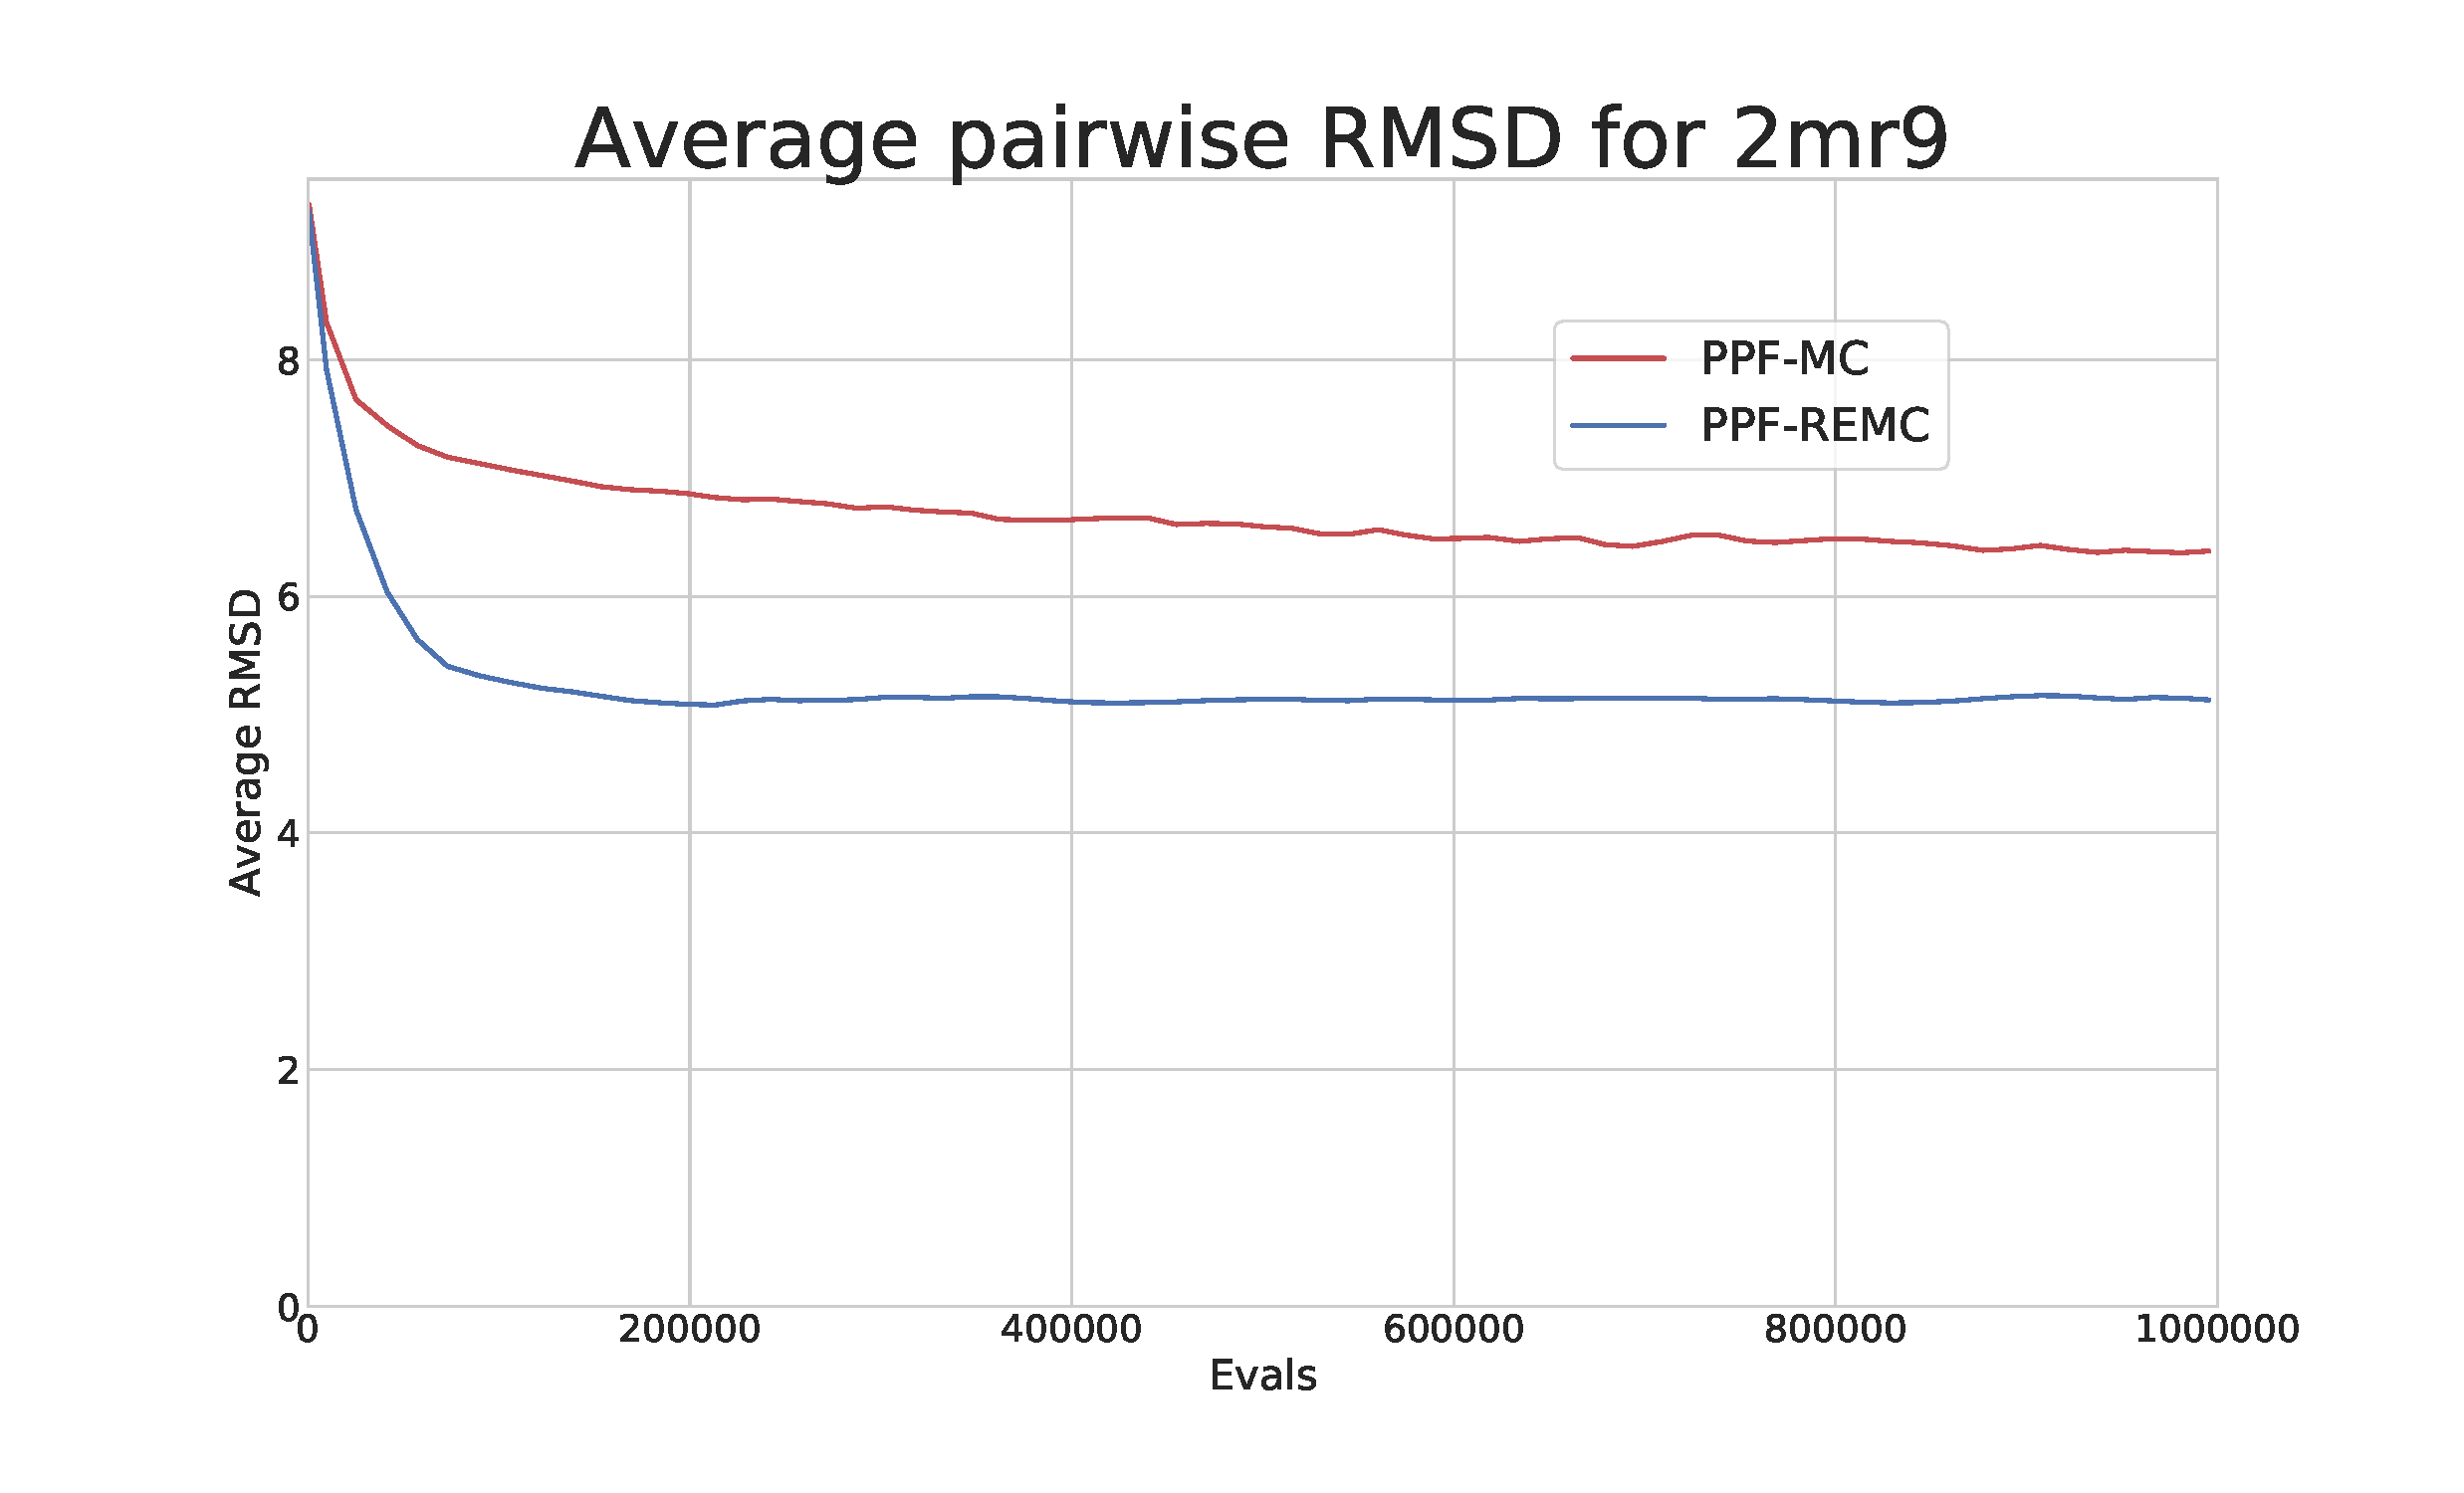
\includegraphics[width=1\linewidth]{Figuras/plots/rmsd_convergence/avg_rmsd_2mr9.pdf}
    \caption{2mr9}
    %\label{fig:2mr9-conformation}
  \end{subfigure}
\end{figure}